\documentclass{book}

\usepackage[left=2.5cm, right=2.5cm, top=2cm, bottom=2cm]{geometry}

% math mode additions
\usepackage{amsmath}
\usepackage{amsfonts}
\usepackage{amssymb}
\usepackage{physics}
\usepackage{slashed}
\usepackage{mathtools}
% nice 3-vectors
\usepackage{esvect}
% nice differentation
% Get straight d's when differantiating
\usepackage[ISO]{diffcoeff}


% appendix
\usepackage[title]{appendix}
% \usepackage[intlimits]{mathtools}

\usepackage[export]{adjustbox}

% in-document references
\usepackage{hyperref}
\usepackage[capitalize]{cleveref}

% create plots
\usepackage{tikz}
\usepackage[compat=1.1.0]{tikz-feynman}
\usepackage{pgfplots}
\pgfplotsset{compat=1.16}

% Nice table of contents
\usepackage{tocloft}

% Get floats right
\usepackage[section]{placeins}

% adjust fig captions
\usepackage{caption}
\usepackage{subcaption}
\captionsetup{width=.9\textwidth}

\usepackage{titlepic}
% \usepackage[textsize=footnotesize]{todonotes}
\usepackage[disable]{todonotes}

\usepackage[style=numeric-comp,sorting=none,sortcites=true,doi=true,url=false,giveninits=true,hyperref]{biblatex}

\setlength{\marginparwidth}{2.2cm}

\setlength\cftparskip{1pt}
\setlength\cftbeforechapskip{0pt}

\setlength{\parindent}{0em}
\setlength{\parskip}{0.8em}

\def\equationautorefname~#1\null{Eq.~(#1)\null}


% Simple shortcuts
\newcommand{\Ell}{\mathcal{L}}      % Lagrangian L
\newcommand{\He}{\mathcal{H}}       % Hamiltonian H
\newcommand{\Ve}{\mathcal{V}}       % Potential V
\newcommand{\Em}{\mathcal{M}}       % Manifold M
\newcommand{\Ef}{\mathcal{F}}       % Fancy f
\newcommand{\R}{\mathbb{R}}         % Real numbers
\newcommand{\chpt}{$\chi$PT }       % Chiral pertubation theory
\newcommand{\SU}{\mathrm{SU}}       % SU(n)
\newcommand{\eps}{\varepsilon}      % nice epsilon
% \newcommand{\one}{\mathbb{1}}       % Identity
\newcommand{\hc}{\mathrm{h.c.}}     % Hermitian conjugate
\newcommand{\ex}[1]{\expectationvalue{#1}}
\newcommand{\D}{\mathcal{D}}

\newcommand{\one}{\text{\usefont{U}{bbold}{m}{n}1}}
\MakeRobust{\one}

% Big-O notation 
\newcommand{\Oh}[2][2]{\mathcal{O}\left(#2^{#1}\right)}

% (anti) commutator
\newcommand{\com}[2]{\left[#1, #2 \right]}
\newcommand{\acom}[2]{\left\{#1, #2 \right\}}

% Lie algebra
\newcommand{\liea}[2]{\mathfrak{#1}\left(#2\right)}
\newcommand{\lieg}[2]{\mathrm{#1}\left(#2\right)}

% Curly brackets
\newcommand{\C}[1]{\left\{ #1 \right\}}

% Fourier Transform
\newcommand{\F}[1]{\mathcal{F}\C{#1}}
\newcommand{\FInv}[1]{\mathcal{F}^{-1}\C{#1}}

% operator in braket
\newcommand{\inner}[3]{\left\langle #1 {\left| #2 \right|} #3 \right\rangle}

\newcommand{\T}[1]{\textrm{T}_\tau \left\{ #1 \right\}}


\title{Chiral Perturbation Theory}
\author{Martin Kjøllesdal Johnsrud}
\titlepic{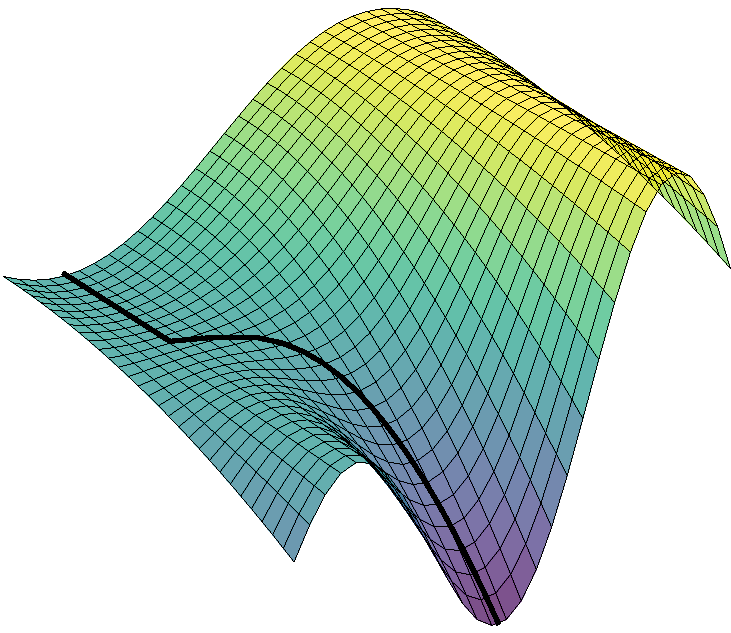
\includegraphics[width=\textwidth]{figurer/numerics/free_energy_surface_wo_axis_cropped.pdf}}

%%%%%%%%%%%%%%%%%%%%
%%%%%%% TODO %%%%%%%
%%%%%%%%%%%%%%%%%%%%

%%%%%%%%%%%%%%%%%%%%%%%%%%%%%%%%%%%%
%%%%%%%%%%%%% SPØRSMÅL %%%%%%%%%%%%%
%%%%%%%%%%%%%%%%%%%%%%%%%%%%%%%%%%%%
% Hvor kommer EOM inn i bildet? Det ser ut som det bare er et navn...
% Hvorfor kan vi bruke EOM fra en annen parametrisering?
% hvorfor er q gamam⁰ q baryontall


%%%%% Kode
% Referer til det

%%%%% TODO: FIN TITTEL!!!

%%%%% INTRO

%%%%% Teori
% Forbedringer:
% Inkluder massive felt

%%%%% Pions

%%%%% Termisk
% Forbedringer:
% Gå gjennom path-integralet for fermioner ordentlig

%%%% Konklusjon

%%%% Kilder
% Fin kildehenvisning, kun initsialer, etc.

%%%%% Thermal field theory

%%%%% Generelt
% Lingningsnummer --- når? - nesten alltid
% Overskrifter --- Stor bokstav? - nei
% være konsekevent på parantes {[()]}
% Alltid bruke cleverref

%%%%% Rettskriving
% Up quark, ikke up-quark
% tree level, ikke the tree level
% Antiquark, ikke anti quark

%%%% Master: To change
% bestem deg for cref eller autoref
% redefiner \Oh
% vær konsekvent på \diff


\begin{document}
\maketitle 

\tableofcontents
\listoftodos

\chapter*{Abstract}
Pions are particles that describe the dynamics of QCD at low energies, and it has recently been proposed that they form compact stellar objects called pion stars.
We use two-flavor chiral perturbation theory to calculate the grand canonical free energy density to next-to-leading order, at $T = 0$ and with non-zero isospin chemical potential $\mu_I$.
\todo{What part is approximate, what is broken? Find out!}
At $\mu_I = m_\pi$, the system breaks the approximate isospin symmetry of the Lagrangian, and we observe the resulting Goldstone mode.
This results in a phase transition to a pion condensate phase with non-zero isospin density.
We discuss the nature of the phase transition using Landua-theory of second-order phase transitions.
The free energy density is used to obtain the relationship between the pressure and the energy density of the system, the equation of state.
This, together with the Tolman–Oppenheimer–Volkoff equation, can be used to model pion stars, allowing for further investigation of these newly proposed objects.


\chapter*{Conventions and notation}
Throughout this text, \emph{natural units} are used.
These units are defined so that
\begin{equation}
    \hbar = c = k_B = 1,
\end{equation}
where $\hbar$ is the Planck reduced constant, $k_B$ is the Boltzmann constant, and $c$ is the speed of light.
These constants will therefore be dropped from all expressions.
They can be reintroduced using dimensional analysis.
In natural units, \emph{mass dimension} is the only engineering dimension.
Dimensionfull results are given in units of electronvolt (eV), or pion-masses, 
\begin{equation}
    m_\pi = 131 \, \text{MeV}.
\end{equation}

The Minkowski metric convention used is the ``mostly minus'',
\begin{equation}
    g_{\mu \nu} = \mathrm{diag}(1, -1, -1, -1).
\end{equation}
The Fourier transform used in this text is defined by
\begin{align*}
    \F{f(x)}(p) = \tilde f(p) = \int \dd x\, e^{i p x}f(x), \quad 
    \FInv{\tilde f(p)}(x) = f(x) = \int \frac{\dd p}{2 \pi}\, e^{- i p x} \tilde f(p).
\end{align*}
We employ the \emph{Einstiein summation convention}, in which pairwise matching indices are summed.
That is,
\begin{equation}
    a_i b_i = \sum_i a_i b_i = a_1 b_1 + \dots.
\end{equation}
For Minkowski-space indices, $\mu$, $\nu$, $\rho$ and $\sigma$, the metric raises and lower indices, and summation should always be over one raised and one lowered index,
\begin{equation}
    a_\mu b^\mu = g_{\mu\nu} a^\mu b^\nu 
    = a^0 b^0 - a^1 b^1 - \dots.
\end{equation}



\chapter{Introduction}
% OUTLINE: 

% - Standard model, QCD

% - Effective Lagrangians,  Weinberg's theorem, symmetry, chiral perturbation theory.

% - Pion stars: calculation of neutron star, not from first principle. Sign problem. Pion stars recently suggested. Equation of state

% - Outline of text

% The standard model describes, together with Einstein's general theory of relativity, all experiments we as humans are able to perform.
The standard model is arguably the most successful theory in all of physics.
It uses the language of quantum field theory to describe the elementary particles of the universe, and their interactions via the electromagnetic, weak and strong forces.
\autoref{fig:the standard model} shows a table of the particles that make up the standard model.
Calculations of the observable quantities using quantum electrodynamics (QED), the quantum theory of electromagnetic interactions, and the theory of weak interactions give highly precise predictions which agrees to an astounding degree with experiments~\cite{Schwartz:QFT}.

These calculations use the techniques of Feynman diagrams, which describes how quantum fields interact as the sum of all possible ways of interaction.
When the interaction is weak, as is the case for QED, we get a sum that converges quickly, and calculating a few orders of the sum will yield highly accurate estimates of phsyical quantities.
The weakness of QED is quantified in the fine structure constant $\alpha \approx 0.00 7297$\cite{PDG}.
A Feynman diagram in QED is proportional to $\alpha^n$, where $n$ is the number of vertices in the diagram, which means the contributions from more complex diagrams with many vertices rapidly becomes insignificant

\begin{figure}
    \centering
    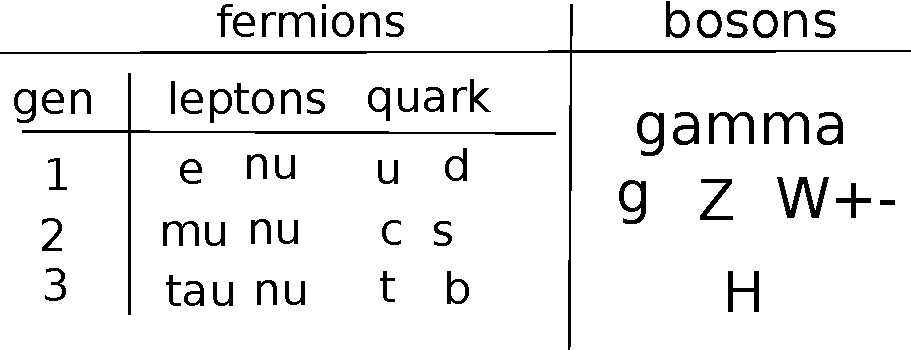
\includegraphics[]{figurer/standard_model.pdf}
    \caption{The particles of the standard model. The fermions are made up of two leptons and two quarks for each generation, for three generations. The photon ($\gamma$) is the particle of the electromagnetic force, the gluon (g) of the strong force, and the $Z$ and $W^\pm$ bosons are responsible for the weak force. The final piece of the puzzle is the Higgs boson (H).}
    \label{fig:the standard model}
\end{figure}

Quantum chromodynamics, or QCD, is the part of the standard model that describes quarks, the constituents of protons and neutrons, and how they interact via the strong nuclear force.
When dealing with the strong force, the fact that the strength of interaction depend on the energy scale of the interaction becomes apparent.
In high energy interactions at the energy scale of the $Z$-boson, $m_z \approx 91.19 \, \text{GeV}$, the strong force equivalent to the fine structure constant is $\alpha_s(m_Z) \approx 0.118$~\cite{PDG}. 
This makes it possible to do perturbative calculations using QCD.
However, the strong force has its name for a reason.
For scales around $1 \text{GeV}$ and below, the perturbation method breaks down.
In this case, quarks bond together and form \emph{hadrons}.
Hadrons are classified as \emph{mesons} or \emph{baryons}.
The most familiar of the baryons are the proton and neutrons.
None of the mesons are stable, but they do play an important role in describing the strong force int the non perturbative regime.
This is done by using \emph{effective field theories}.

\subsection*{Effective field theories}

A profound feature of physics is the possibility of describing a system by isolating the degrees of freedom of interest, and ignoring the rest.
We can describe the motion of the planets in the solar system, massive and complex systems, by only their mass, velocity and position.
In quantum field theory, this feature manifests in the power of effective field theory.
An effective field theory describes a system not by the fundamental, underlying particles, whatever that may mean, but by effective fields.
A theory of two interacting fields $\varphi$ and $\psi$ will be described by an action which depends on both fields, $S[\varphi, \psi]$.
In the path integral formalism, predictions can be then be made by integrating over all possible states for these fields.
An exmple is the vacuum transition amplitude,
\begin{equation}
    Z = \int \D \varphi \D \psi \, \exp{i S[\varphi, \psi]}.
\end{equation}
The effective description of only the $\varphi$-degrees of freedom by \emph{integrating out} the $\psi$-degrees of freedom, which results in an effective action $S_\text{eff}[\varphi]$, defined by~\cite{Schwartz:QFT}
\begin{equation}
    \label{integrating out degrees of freedom}
    \int D \varphi \, \exp{i S_\text{eff}[\varphi]} 
    =
    \int \D \varphi \D \psi \, \exp{i S[\varphi, \psi]}.
\end{equation}
This gives us hope for describing low energy QCD as an effective theory of the particles we know from experiments appear.
In this text, we will derive and explore an effective theory of the pionic degrees of freedom of low-energy QCD, called chiral perturbation theory, or \chpt.

Mesons, of which pions are the lightest, were first proposed by Hideki Yukawa as the mechanism to hold nucleons together to form the nucleus of atoms.
Though first believed to appear in the showers of particles that comes from cosmic rays, they were decisively discovered in 1947, by Cecil F. Powell \emph{et. al.}~\cite{griffiths:introduction}
Pions do not show up in the standard model, as quarks do, but rather as an effective degree of freedom at low temperature.
The action of the standard model has a very particular, nice form.
It is the integral over a local Lagrangian, that is
\begin{equation}
    S[\varphi] = \int \dd^4 x \, \Ell[\varphi].
\end{equation}
Here, we denote all particles by $\varphi$.
That the Lagrangian $\Ell$ is local means that it is made up of terms like $\varphi(x) \varphi(x)$, all interactions happens at one point in space-time, as opposed to a term such as $f(x, y)\varphi(x) \varphi(y)$.
We can not a priori expect an effective action to take this form~\cite{Schwartz:QFT}.
However, we have general principles we expect particles to obey, such Lorentz invariance and cluster decomposition.
Cluster decomposition concerns a system of $N$ sets of particles, $\alpha_i$, that evolve into the sets $\beta_i$.
That is,
\begin{equation}
    \ket{\alpha_1, \alpha_2, ... \alpha_N}_\text{in}
    \longrightarrow
    \ket{\beta_1, \beta_2, ... \beta_N}_\text{out}.
\end{equation}
It says that if the sets of particles $\alpha_i$, $\beta_i$ are located far enough apart, then the $S$-matrix factors as
\begin{equation}
    {\braket{\beta_1, \beta_2, ... \beta_N}{\alpha_1, \alpha_2, ... \alpha_N}}
    =
    \braket{\beta_1}{\alpha_1}\braket{\beta_2}{\alpha_2}... \braket{\beta_N}{\alpha_N}.
\end{equation}
This is a familiar property, as it essentially says that wildly separated experiments do not interfere, and one that we expect all good effective description to have~\cite{weinberg_1995,weinberg_1996_vol2}.

The method we use to construct the effective action of \chpt is one formulated by Weinberg.
This method relies on, as Weinberg himself called it, a ``theorem'':
\begin{quote}
    [I]f one writes down the most general possible Lagrangian, including all terms consistent with assumed symmetry principles, and then calculates matrix elements with this Lagrangian to any given order of perturbation theory, the result will simply be the most general possible S-matrix consistent with analyticity, perturbative unitary, cluster decomposition and the assumed symmetry principles. \cite{WeinbergPhenom}
\end{quote}
In other words, if we write down the most general Lagrangian consistent with symmetries of the underlying theory, then we have not made any restrictions on the theory, other than some foundational assumptions.
This Lagrangian will be on the form
\begin{equation}
    \Ell_\text{eff}[\varphi] = \sum_i \lambda_i \mathcal O_i,
\end{equation}
where $\mathcal O_i$ are local functions of the fields and its derivatives, and $\lambda_i$ are coupling constants.
The coupling constants are free parameters, which parametrizes the most general $S$-matrix consistent with fundational assumptions and the underlying theory.
A Lagrangian with an infinite amount of free parameters might seem useless, however if we are able to find a consistent series expansion, then only a finite number of terms are needed to calculate to any given order in perturbation theory.
In the case of \chpt, the expansion is in the energy of the pions.
We will detail this later in the text.


\subsection*{Stars}

Although it might seem counterintuitive, stars are one of the objects we might hope to describe using QCD at low energies.
Neutron stars, one of the most extreme objects in the universe, quickly cools down to temperatures below $10^{10} \, \text{K}$.
This might be hot by almost all standards, however it corresponds to an energy of $0.862 \, \text{MeV}$.
This is well into the strong interaction regime of QCD, and the stars must therefore be described by an effective theory of interacting nuclear matter~\cite{glendenning:compcat_stars,from_hadrons_to_quarks}.
Stars are modeled using the Tolman-Oppenheimer-Volkoff, or TOV, equation.
The TOV equation is based on Einstein's general theory of relativity, and its solution gives the pressure of the star as a function of its radius.
The only input needed is the \emph{equation of state}, or EOS, of the material that makes up the star~\cite{Carroll:spacetime}.
The equation of state of a material is the relationship between its energy density, $u$, and pressure $P$, i.e. a relationship of the form
\begin{equation}
    f(P, u) = 0.
\end{equation}
This is where QCD comes in.
One way to compute the equation of state of QCD systems is using the lattice QCD, a numerical method.
Here, space-time is approximated as finite and discrete, and Monte-Carlo importance sampling is used to perform the path integral.
This method, however, fails for non-zero baryon densities in what is known as the fermion sign problem.
Non-zero baryon density, or equivalently non-zero baryon chemical potential $\mu_B$, corresponds to systems with a matter-antimatter asymmetry, such as neutron stars, or more generally all observed stars.
Recently, it has been proposed that a condenset of pions can form a new type of compact, gravitationally bound object, i.e. a star.
States of pion condensates can have zero baryon chemical potential, and are thus amenable to lattice QCD simulations.
This offer a way to model stellar objects from first principles, as well as by analytical methods using \chpt~\cite{new_clas_of_compact_stars,andersen:bose_einstein}.

\subsection*{Pion condensate and the QCD phase diagram}
(Isospin: \cite{Brandt:QCD_phase_diagram_with_isospin_chemical_potential,PhysRevD.97.054514}
baryon: \cite{from_hadrons_to_quarks,Fukushima:The_phase_diagram_of_dense_QCD})

A pion condensate is a state with a non-zero expectation value of pions, $\ex{\pi} \neq 0$.
The condensation happens when the pion chemical potential reaches a chritical value, $\mu_I = \mu_I^c$.
This is just one part of the rich phase structure of QCD.
The full phase diagram is not yet known, due to the many difficulties, some of which are mentioned in this text.
At low temperatures and chemical potentials, in the normal or vacumm phase, we get a hadronic gas.
For high temperature or chemical potentials, we get a quark gluon plasma.
In this phase, quarks are no longer tightly bound in hadrons, but together with gluons form as soup conjectured to be at the center of neutron stars.(SIKKER? KILDE)
For high (HOW) baryon chemical potential, we expect that there forms a color super conductor (KILDE).
Better understanding of the phase diagram of QCD is a large part of understanding the standard model and its consequences better.
To be able to validate the techniques used, it is important to employ all possible, sound approaches.
This makes it possible to crosscheck techniques, such as when comparing \chpt with lattice QCD.

\begin{figure}
    \centering
    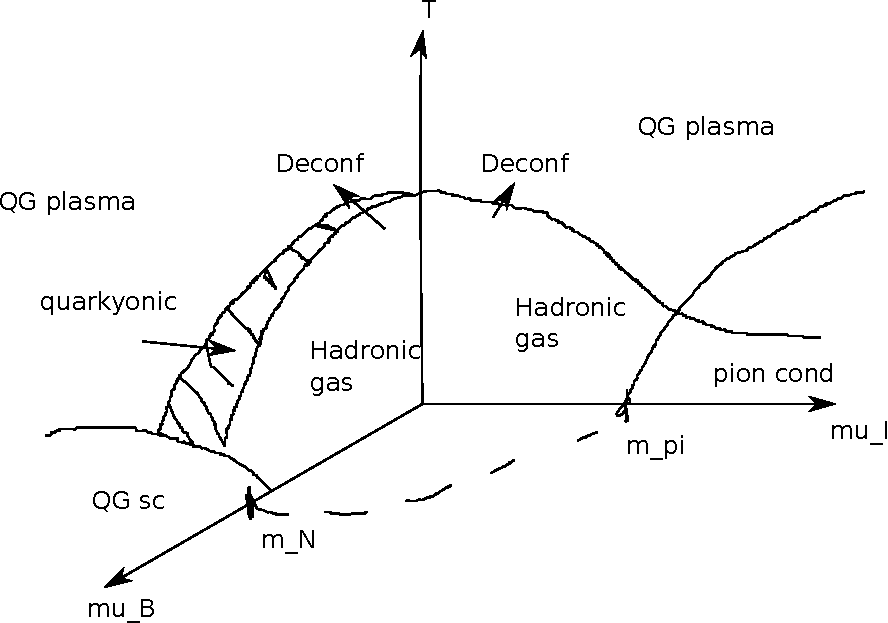
\includegraphics[]{figurer/phase_diagram.pdf}
    \caption{(KLADD) The phase diagram of QCD}
    \label{fig:phase diag qcd}
\end{figure}

\subsection*{Outline of thesis}
The goal of this thesis is to calculate the next-to-leading order equation of state of a system at finite isospin chemical potential, using two-flavor chiral perturbation theory.
We will also investigate the phase transition from the vacuum phase into a pion condensate phase.
In \cref{chapter:theory}, we take a survey of some general theory needed for \chpt.
We start by introducing the generating functional in the path integral formalism, and use this to define the one-praticle-irreducible effective action, and the effective potential.
This allows us to prove Goldstone theorem, an important result which provides the connection between the symmetries of a theory, and its low energy dynamics.
The theorem states that a system which undergoes spontaneous symmetry breaking gives rise to massless particles.
We then present the CCWZ construction, which provides a procedure to constructs an effective Lagrangian of Goldstone bosons.
We also present some mathematical prerequisite, such as Lie groups and Lie algebras, and discuss the role and mathematical implementation of symmetry in physics in general and quantum field theory in particular.
In \autoref{chapter:effective theory of pions}, we take the general theory of the last chapter, and apply it to QCD to get \chpt.
We start the chapter by discussing QCD, its constituent parts and their symmetries and the corresponding conserved currents.
We then use the theory from last chapter to find the terms with makes up the Lagrangian of \chpt, as well as how to incorporate explicit breaking of symmetry and external source currents, as well as a finite isospin chemical potential.
This section also contains a discussion about how to order these terms in a well-defined series expansion, and avoid the need to include infinity many terms.
With this, we construct the leading order and next-to-leading order Lagrangian, which is expanded in powers of the pion fields.
We discuss how to identify possible redundant terms in the Lagrangian, and use our result to find properties of the pion such as their tree-level mass and propagator.
In \autoref{chapter:thermodynamics}, we use our result to calculate the free energy density, to one loop using the leading order Lagrangian, and then use the tree level result at next-to-leading order to renormalize the result.
We discuss the low energy parameters we use, and how to evaluate observable to the same order in perturbation theory consistently.
With the free energy density, we explore the thermodynamics of pions at finite isospin chemical potential, and derive the equation of state.
We also discuss the phase transition to the pion condensate phase using the Landau theory of phase transition.
In \autoref{chpater:conclusion and outlook}, we (SKRIV KAPITTEL!!!!)

The appendix is referenced throughout the text, to keep the thesis as self-contained as possible.
In \autoref{appendix:thermal field theory}, we review thermal field theory and the imaginary time formalism.
This chapter contains calculations needed in the main part of the thesis, where they are referenced, and lays out the path integral approach as well as its connection to thermodynamics in more detail.
We also discuss dimensional regularization, derive the Feynman rules for and interacting scalar and generalize thermal field theory to fermions.
\autoref{appendix:conventions and notaition} summarize the convention and notation used in this thesis, as well as discussing some of the used in the thesis mathematics in more detail.





\chapter{Theory}
\label{chapter:theory}

\label{Free energy and the effective action}
The theory in this section is based on \cite{Peskin:IntroQFT,weinberg_1995,weinberg_1996_vol2,Schwartz:QFT}.
Feynman diagrams are drawn using JaxoDraw~\cite{JaxoDraw}.

\subsection{QFT via path integrals}
\label{section:path integral}
The vacuum transition amplitude is given by the path integral
\begin{equation}
    Z = \lim_{T\rightarrow \infty} \braket{\Omega, T/2}{-T/2, \Omega}
    = \lim_{T\rightarrow \infty} \inner{\Omega}{ e^{-iHT} }{\Omega}
    = \int \D \pi \D \varphi \, \exp{ i \int \dd^4 x \, \left(\pi \dot \varphi - \He[\pi, \varphi]\right) },
\end{equation}
where $\ket{\Omega}$ is the vacuum of the theory.
By introducing a source term into the Hamiltonian density, $\He \rightarrow \He - J(x)\varphi(x)$, we get the generating functional
\begin{equation}
    Z[J] = 
    \int \D \pi \D \varphi \, 
    \exp{ i \int \dd^4 x \, \left(\pi \dot \varphi - \He[\pi, \varphi]+ J\varphi\right) }.
\end{equation}
If $\He$ is quadratic in $\pi$, we can complete the square and integrate out $\pi$ to obtain
\begin{equation}
    Z[J] = C \int \D \varphi \, \exp{i \int \dd^4 x\, (\Ell[\varphi] + J \varphi)}.
\end{equation}
$C$ is infinite, but constant, and will drop out of physical quantities.
In scattering theory, the main objects of study are correlation functions $\ex{\varphi(x_1)\varphi(x_2)...} = \inner{\Omega}{T\left\{\varphi(x_1)\varphi(x_2)\dots\right\}}{\Omega}$, where $T$ is the time ordering operator.
These are given by functional derivatives of $Z[J]$, 
\begin{equation}
    \label{correlator from generating functional}
    \ex{\varphi(x_1)\varphi(x_2)...}
    = 
    \frac{\int \D \varphi(x)\,  (\varphi(x_1)\varphi(x_2)...) e^{i S[\varphi]}}
        {\int \D \varphi(x)\, e^{i S[\varphi]}}
    =
    \frac{1}{Z[0]} \prod_i\left( -i  \fdv{J(x_i)}\right) Z[J]\Big|_{J = 0},
\end{equation}
where 
\begin{equation}
    S[\varphi] = \int \dd^4 x \, \Ell[\varphi]
\end{equation}
is the action of the theory.
The functional derivative is described in \autoref{section:Functional derivative}.
In a free theory, we are able to write
\begin{equation}
    Z_0[J] = Z_0[0] \exp(i W_0[J]), \quad 
    W_0[J] = \frac{1}{2} \int \dd^4 x \dd^4 y \, J(x) D_0(x - y) J(y),
\end{equation}
where $D_0$ is the propagator of the free theory.
Using this form of the generating functional, \autoref{correlator from generating functional} becomes
\begin{align*}
    & \frac{1}{Z[0]}  (-i)^n\fdiff{}{J(x_1)} ... \fdiff{}{J(x_n)} Z_0[J]  \Big|_{J = 0}
    = (-i)^n \fdiff{}{J(x_1)} ... \fdiff{}{J(x_n)} e^{i W_0[J]} \Big|_{J = 0}\\
    & = (-i)^{n} \fdiff{}{J(x_1)} ... \fdiff{}{J(x_{n-1})} \left(i \fdiff{W_0[J]}{ J(x_{n}) } \right) e^{i W_0[J]} \Big|_{J = 0}\\
    & = (-i)^{n}\fdiff{}{J(x_2)} ... \fdiff{}{J(x_{n-1})}
    \left(
        i\fdiff{ W_0[J] }{ J(x_{n-1}), J(x_{n}) }
        + i^2 \fdiff{W_0[J]}{J(x_{n-1})} \fdiff{W_0[J]}{J(x_{n})}
    \right) 
    e^{i W_0[J]} \Big|_{J = 0}
    = \dots \\
    &= 
    (- i )^{n/2}\sum_{{(a, b)}} \prod_{i=1}^{n/2}
    \fdiff{ W_0[J] }{ J(x_{a(i)}), J(x_{b(i)}) } \Big|_{J = 0}.
\end{align*}
In the last line we have introduced the functions $a, \, b$ which define a way to pair up $n$ elements.
The domain of the functions are the integers between $1$ and $n/2$, the image a subset of the integers between $1$ and $n$ of size $n/2$.
A valid pairing is a set $\{(a(1), b(1)), \dots (a(n/2), b(n/2))\}$, where all elements $a(i)$ and $b(j)$ are different, such all integers up to and including $n$ are featured.
A pair is not directed, so $(a(i), b(i))$ is the same pair as $(b(i), a(i))$.
The sum is over the set ${\{(a, b)\}}$ of all possible, unique pairings.
If $n$ is odd, the expression is equal to $0$.
This is Wick's theorem, and it can more simply be stated as \emph{a correlation function is the sum of all possible pairings of 2-point functions},
\begin{equation}
    \ex{{\prod}_{i=1}^{n} \varphi(x_i)  }_0
    = \sum_{\{(a, b)\}}  \prod_{i=1}^n  \ex{\varphi(x_{a(i)}) \varphi(x_{b(i)})}_0.
\end{equation}
The subscript on the expectation value indicates that it is evaluated in the free theory.

If we have an interacting theory, that is a theory with an action $S = S_0 + S_I$, where $S_0$ is a free theory, the generating functional can be written
\begin{equation}
    \label{partition function of interacting theory.}
    Z[J] 
    = Z_0[0] \ex{\exp(iS_I + i\int \dd^4 x \, J(x) \varphi(x))}_0.
\end{equation}
We can expand the exponential in power series, which means the expectation in \autoref{partition function of interacting theory.} becomes
\begin{equation}
    \sum_{n, m} \frac{1}{n! m!} \ex{(iS_I)^n \left(i\int \dd^4 x \, J(x) \varphi(x)\right)^m}_0.
\end{equation}
The terms in this series are represented by Feynman-diagrams, which are constructed from the Feynman-rules, and can be read from the action.
We will not go into further details on how the Feynman-rules are derived, which can be found in any of the main sources for this section~\cite{Peskin:IntroQFT,weinberg_1995,weinberg_1996_vol2,Schwartz:QFT}.
The source terms gives rise to an additional vertex
\begin{equation}
    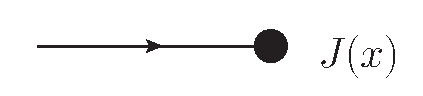
\includegraphics[width=0.25\textwidth, valign=c]{figurer/feynman-diagram/cnt_vertex.eps}.
\end{equation}
The generating functional $Z[J]$ equals $Z_0[0]$ times \emph{the sum of all diagrams with external sources $J(x)$}.
% The expectation value
% \begin{equation}
%     \ex{(iS_I)^n (\varphi(x)J(x))^m}_0
% \end{equation}
% are all diagrams with $n$ vertices given by the Feynman rules from the interacting action $S_I$, as well as $m$ m source vertices.

Consider a general diagram without external legs, built up of $N$ different connected subdiagrams, where subdiagram $i$ appears $n_i$ times.
As an illustration, a generic vacuum diagram in $\phi^4$-theory has the form
\begin{align}
    \label{Feinman diagrams}
    V = 
    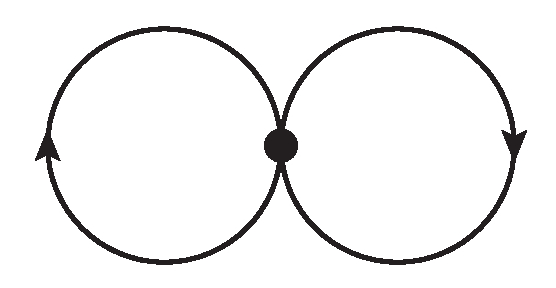
\includegraphics[width=0.1\textwidth, valign=c]{figurer/feynman-diagram/phi-4_loop_notext.eps}
    \times
    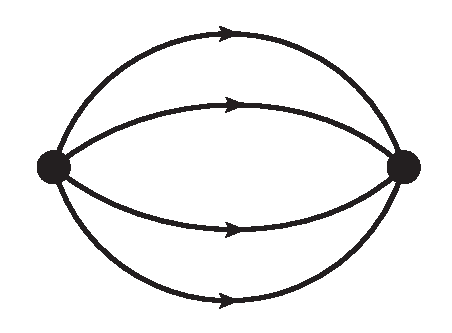
\includegraphics[width=0.08\textwidth, valign=c]{figurer/feynman-diagram/phi-4_2_loop.eps}
    \times
    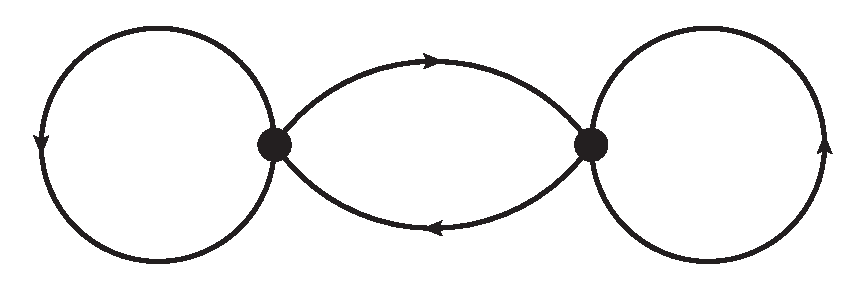
\includegraphics[width=0.14\textwidth, valign=c]{figurer/feynman-diagram/phi-4_2_loop2.eps}
    \times
    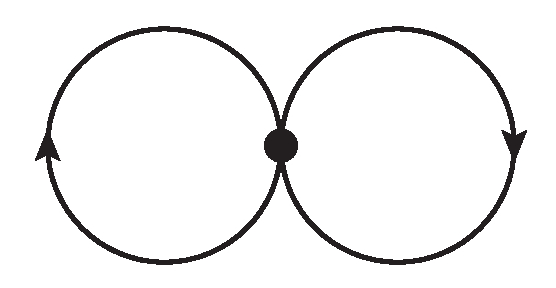
\includegraphics[width=0.1\textwidth, valign=c]{figurer/feynman-diagram/phi-4_loop_notext.eps}
    \times \dots.
\end{align}
If sub-diagram $i$ as a stand-alone diagram equals $V_i$, then each copy of that subdiagram contribute a factor $V_i$ to the total diagram.
However, due to the symmetry of permuting identical subdiagrams, one must divide by the extra symmetry factor $s = n_i !$, which is the total number of permutation of all the copies of diagram $i$.
The value of the total diagram is therefore
\begin{align}
    \label{Feynman diagrams}
    V
    = \prod_{i= 1}^N \frac{1}{n_i!} V_i^{n_i}.
\end{align}
$V$ is uniquely defined by a finite sequence of integers, $(n_1, n_2, \dots n_N, 0, 0, \dots)$, so the sum of all diagrams is the sum over the set $S$ of all finite sequences of integers.
This allows us to write the sum of all diagrams as
\begin{equation}
    \label{sum of all diagrams}
    \sum_{(n_1, ...)\in S} \prod_{i} \frac{1}{n_i!} V_i^{n_i}
    = \prod_{i = 1}^{\infty} \sum_{n_i=1}^{\infty} \frac{1}{n_i!} V_i^{n_i}
    = \exp({\sum}_i V_i).
\end{equation}
We showed that the generating functional $Z[J]$ were the $Z_0[0]$ times the sum of all diagrams due to external sources.
Using \autoref{sum of all diagrams}, we see that the sum of all \emph{connected} diagrams $W[J]$ is given by
\begin{equation}
    Z[J] = Z_0[0]\exp(i W[J]).
\end{equation}
We can see that this is trivially true for the free theory, the only connected diagram is
\begin{equation}
    \label{generating functional of connected diagrams}
    W_0[J] = 
    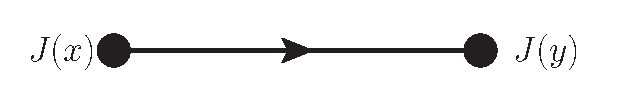
\includegraphics[valign=c, width=0.3\textwidth]{figurer/feynman-diagram/current-current.eps}.
\end{equation}

\section{The 1PI effective action and the effective potential}

\label{section: effective action}
The generating functional for connected diagrams, $W[J]$, is dependent on the external source current $J$.
Analogously to what is done in thermodynamics and in Lagrangian and Hamiltonian mechanics, we can define a new quantity, with a different independent variable, using the Legendre transformation.
The new independent variable is 
\begin{equation}
    \varphi_J(x) := \frac{\delta W[J]}{\delta J(x)} = \ex{\varphi(x)}_J.
\end{equation}
The subscript $J$ on the expectation value indicate that it is evaluated in the presence of a source.
The Legendre transformation of $W$ is then
\begin{equation}
    \label{1PI effective action}
    \Gamma[\varphi_J]
    = W[J] - \int \dd^4 x \, J(x) \varphi_J(x).
\end{equation}
Using the definition of $\varphi_J$, we have that
\begin{equation}
    \label{effective equation of motion}
    \fdv{\varphi_J(x)} \Gamma[\varphi_J]
    = \int \dd^4 y \, \fdv{J(y)}{\varphi_J(x)} \fdv{J(y)} W[J]
    - \int \dd^4 y \, \fdv{J(y)}{\varphi_J(x)} \varphi_J(y)
    - J(x)
    = - J(x).
\end{equation}
If we compare this to the classical equations of motion of a field $\varphi$ with the action $S$,
\begin{equation}
    \frac{\delta S[\varphi]}{\delta \varphi(x)} = -J(x),
\end{equation}
we see that $\Gamma$ is an action that gives the equation of motion for the expectation value of the field, given a source current $J(x)$.

To interpret $\Gamma$ further we observe what happens if we treat $\Gamma[\varphi]$ as a classical action with a coupling $g$.
The generating functional in this new theory is
\begin{equation}
    \label{partition function with g}
    Z[J, g] = \int \D \varphi 
    \exp{ i g^{-1} \left( \Gamma[\varphi] + \int \dd^4x \varphi(x) J(x) \right) }
\end{equation}
The free propagator in this theory will be proportional to $g$, as it is given by the inverse of the equation of motion for the free theory.
All vertices in this theory, on the other hand, will be proportional to $g^{-1}$, as they are given by the higher order terms in the action $g^{-1}\Gamma$.
This means that a diagram with $V$ vertices and $I$ internal lines is proportional to $g^{I-V}$.
Regardless of what the Feynman-diagrams in this theory are, the number of loops of a connected diagram is $L = I - V + 1$.
\footnote{This is a consequence of the Euler characteristic $\chi = V - E + F$.}
To see this, we first observe that one single loop must have equally many internal lines as vertices, so the formula holds for $L = 1$.
If we add a new loop to a diagram with $n$ loops by joining two vertices, the formula still holds.
If we attach a new vertex with one line, the formula still holds, and as the diagram is connected, any more lines connecting the new vertex to the diagram will create additional loops.
This ensures that the formula holds, by induction.
As a consequence of this, any diagram is proportional to $g^{L-1}$.
This means that in the limit $g \rightarrow 0$, the theory is fully described at the tree-level, i.e. by only considering diagrams without loops.
In this limit, we may use the stationary phase approximation, as described in \autoref{section:gaussian integrals}, which gives
\begin{equation}
    Z[J, g\rightarrow 0] \approx 
    C \det(- \frac{\delta^2 \Gamma[\varphi_J]}{\delta \varphi^2})
    \exp{i g^{-1} \left(\Gamma[\varphi_J] + \int \dd^4x J \varphi_J \right)  }.
\end{equation}
This means that
\begin{equation}
    -i g \ln(Z[J, g]) 
    = g W[J, g] 
    = \Gamma[\varphi_J] + \int \dd^4x\,  J(x) \varphi_J(x) + \mathcal{O}(g),
\end{equation}
which is exactly the Legendre transformation we started out with, modulo the factor $g$.
$\Gamma$ is therefore the action which describes the full theory at the tree level.
For a free theory, the classical action $S$ equals the effective action, as there are no loop diagrams.

The propagator $D(x, y)$, which is the connected 2 point function $\ex{\varphi(x)\varphi(y)}_J$, is given by the second functional derivative of $W[J]$, times $-i$.
Using the chain rule, together with \autoref{effective equation of motion}, we get
\begin{align}
    (-i)\int \dd^4 z \frac{\delta^2 W[J]}{\delta J(x) \delta J(z)} 
    \frac{\delta^2 \Gamma[\varphi_J]}{\delta \varphi_J(z) \varphi_J(y)}
    =
    (-i)\int \dd^4 z \frac{\delta \varphi_J[z]}{\delta J(x)}
    \frac{\delta^2 \Gamma[\varphi_J]}{\delta \varphi_J(z) \varphi_J(y)}
    =
    \fdiff{}{J(x)}  \fdiff{\Gamma[\varphi_J]}{\varphi_J(y)}
    = \delta(x - y).
\end{align}
This shows that the second functional derivative of the effective action is $iD^{-1}$, where $D^{-1}$ is the inverse propagator.
The inverse propagator is the sum of all one-particle-irreducible (1PI) diagrams, with two external vertices.
More generally, $\Gamma$ is the generating functional for 1PI diagrams, which is why it is called the 1PI effective action.

% The expectation value of the ground state field configuration, that is at $J=0$, $\ex{\varphi(x)}_{J=0} = \varphi_0(x)$ obeys the equation of motion
% \begin{equation}
%     \frac{\delta \Gamma[\varphi_0]}{\delta \varphi(x)} = 0.
% \end{equation}
For a constant field configuration $\varphi(x) = \varphi_0$, the effective action, which is a functional, becomes a regular function.
We define the effective action $\Veff$ by
\begin{equation}
    \label{definition effective potential}
    \Gamma[\varphi_0] = - V T \, \Ve_{\mathrm{eff}}(\varphi_0),
\end{equation}
$VT$ is the volume of space-time.
For a constant ground state, the effective potential will equal the energy of this state.
To calculate the effective potential, we can expand the action around this state to calculate the effective action,
by changing variables to $\varphi(x) = \varphi_0 + \eta(x)$.
$\eta(x)$ now parametrizes fluctuations around the ground state, and has by assumption a vanishing expectation value.
The generating functional becomes
\begin{align}
    Z[J] 
    = \int \D (\varphi_0 + \eta) \, 
    \exp{i S[\varphi_0 + \eta] + i \int \dd^4 x J (\varphi_0 + \eta) }
\end{align}
The notation 
\begin{equation}
    \fdiff{S[\varphi_0]}{\varphi(x)}
\end{equation}
indicates that the functional $S[\varphi]$ is differentiated with respect to $\varphi(x)$, then evaluated at $\varphi(x) = \varphi_0$.
The functional version of a Taylor expansion is
\begin{equation}
    S[\varphi_0 + \eta] = 
    S[\varphi_0]
    + \int \dd x \fdv{S[\varphi_0]}{\varphi(x)} \eta(x)
    + \frac{1}{2} \int \dd x \dd y\,  \frac{\delta^2 S[\varphi_0]}{\delta\varphi(x)\delta\varphi(y)} \eta(x) \eta(y)
    + \dots
\end{equation}
We will only consider this expansion up to second order in derivatives for now.
Inserting this into $Z[J]$ we get
\begin{align*}
    &Z[J] = \\ 
    &\int \D \eta  
    \exp{
        i \int \dd^4 x \left(  \Ell[\varphi_0] + J \varphi_0  \right)
        + i \int \dd^4x \left(  \fdv{S[\varphi_0]}{\varphi(x)} + J(x) \right) \eta(x)
        + i \frac{1}{2} \int \dd^4 x \dd^4 y \,  
        \frac{\delta^2 S[\varphi_0]}{\delta\varphi(x)\delta\varphi(y)} \eta(x) \eta(y)
        }
\end{align*}
The first term is constant with respect to $\eta$, and may therefore be taken outside the path integral.
The second term gives rise to tadpole diagrams, which alter the expectation value of $\eta(x)$.
For $J=0$, this expectation value should vanish, so this term can be ignored.
Furthermore, this means that the ground state must minimize the classical potential,
\begin{equation}
    \label{minimize classical potential}
    \diffp{\Ve(\varphi_0)}{\varphi} = 0.
\end{equation}

The one loop approximation to the effective potential is given by the Taylor-expansion up to second order.
This term is a Gaussian integral, and may be evaluated as described in \autoref{section:gaussian integrals},
\begin{equation}
    \int \D \eta \, 
    \exp(
        i \frac{1}{2} \int \dd^4x \dd^4y\,  
        \frac{\delta^2 S[\varphi_0]}{\varphi(x)\varphi(y)} \eta(x) \eta(y)
        )
        = C \det\left( - \fdiff{S[\varphi_0]}{\varphi(x), \varphi(y)} \right)^{-1/2}
\end{equation}
The generating functional for connected diagrams, as defined in \cref{generating functional of connected diagrams}, is therefore
\begin{align}
    \label{generating functional}
    W[J] 
    & = 
    \int\dd^4 x \, \left(\Ell[\varphi_0] + J \varphi_0\right)
    +i \frac{1}{2} \Tr{\ln\left( - \fdiff{S[\varphi_0]}{\varphi(x), \varphi(y)}  \right)}
    + \dots,
\end{align}
where we have used the identity $\ln \det M = \Tr \ln M$.
Using the definition of the effective action, \cref{1PI effective action}, and \cref{definition effective potential} we get an explicit formula for the effective potential to 1 loop order,
\begin{equation}
    \label{effective potential}
    \Veff(\varphi_0) = \Ve(\varphi_0) - \frac{i}{VT}  \frac{1}{2} \Tr{\ln\left( - \fdiff{S[\varphi_0]}{\varphi(x), \varphi(y)}  \right)}.
\end{equation}

\section{Symmetry and Goldstone's theorem}
\label{section:symmetry}

This section is based on \cite{Peskin:IntroQFT,weinberg_1995,weinberg_1996_vol2,smooth_manifolds}.

The symmetries of a theory are transformations of the physical state that leave the governing equations unchanged.
A lot of physics is contained in the symmetries of a theory, such as the presence of conserved quantities and the systems low energy behavior.
We distinguish between internal and external symmetries.
An external symmetry is an active coordinate transformation, such as rotations or translations.
They relate degrees of freedom at different space-time points, while internal symmetry transforms degrees of freedom at each space-time point independently of what happens at other points.
A further distinction is between local and global symmetry transformations.
Local transformations have one rule for how to transform degrees of freedom at each point, which is applied everywhere, while local transformations might themselves be functions of space-time.

In classical field theory, symmetries are encoded in how the Lagrangian changes due to a transformation of the fields.
We will consider continuous transformations, which are can in general be written as
\begin{equation}
    \varphi(x) \longrightarrow \varphi'(x) = f_t[\varphi](x), \quad t \in [0, 1].
\end{equation}
Here, $f_t[\varphi]$ is a functional in $\varphi$, and a smooth function of $t$, with the constraint that $f_0[\varphi] = \varphi$.
This allows us to look at ``infinitesimal'' transformations,
\begin{equation}
    \label{infinitesimal transformation}
    \varphi'(x) = f_\epsilon[\varphi] \sim \varphi(x) + \epsilon\diff{f[\varphi]}{t}\bigg |_{t=0}, \quad \epsilon \rightarrow 0.
\end{equation}
We will consider internal, global transformations which act as linearly on $\varphi$.
For $N$ fields, $\varphi_i$, this can be written
\begin{equation}
    \label{linear field transformation}
    \varphi_i'(x) = \varphi_i(x) + \epsilon \, i t_{ij} \varphi_j(x), \quad \epsilon \rightarrow 0.
\end{equation}
$t_{ij}$ is called the generator of the transformation.
A symmetry of the system is then one in which the Lagrangian is unchanged by the transformation, or at most is different by a divergence-term.
That is, a transformation $\varphi \rightarrow \varphi'$ is a symmetry if 
\begin{equation}
    \Ell[\varphi'] = \Ell[\varphi] + \partial_\mu K^\mu[\varphi],
\end{equation}
where $K^\mu[\varphi]$ is a functional of $\varphi$.\footnote{Terms of the form $\partial_\mu K^\mu$ does not affect the physics, as variational principle $\delta S = 0$ do not vary the fields at infinity.}
This is a requirement for a symmetry in quantum field theory too.
However, as physical quantities in quantum field theory are given not just by the action of a single state but the path integral, the integration measure $\D \varphi_i$ has to be invariant as well.
If a classical symmetry fails due to the integration measure, it is called an anomaly.

To investigate the symmetry properties of a quantum theory, we explore what constraints a symmetry lies on the effective action.
To that end, assume 
\begin{equation}
    \D \varphi'(x) = \D \varphi(x), \quad
    S[\varphi'] = S[\varphi].
\end{equation}
In the generating functional, such a transformation corresponds to a change of integration variable.
Using the infinitesimal version of the transformation, we may write
\begin{align}
    Z[J] 
    = \int \D \varphi \, \exp{i S[\varphi] + i \int \dd^4 x J_i(x) \varphi_i(x)} 
    = \int \D \varphi' \, \exp{i S[\varphi'] + i \int \dd^4 x J_i(x) \varphi'_i(x)}
    \\
    = Z[J] -  \epsilon \int \dd^4 x J_i(x) \int \D \varphi \, e^{i S[\varphi]} [t_{ij} \varphi_j(x)],
\end{align}
Using \cref{effective equation of motion}, we can write this as
\begin{equation}
    \label{effective action symmetry requirement}
    \int \dd^4 x \, \fdiff{\Gamma[\varphi_J]}{\varphi_i(x)} \, t_{ij}\ex{\varphi_j(x)}_J = 0.
\end{equation}
This constraint will allow us to deduce the properties of a theory close to the ground state, only using information about the symmetries of the theory.


The arch typical example of an internal, global and continuous symmetry is the linear sigma model, which we will use as an example throughout this section.
The linear sigma model is made up of $N$ real scalar fields $\varphi_i$, which are governed by the Lagrangian
\begin{equation}
    \Ell[\varphi] 
    = \frac{1}{2} \partial_\mu \varphi_i(x) \partial^\mu \varphi_i(x) - \Ve(\varphi),
    \quad \Ve(\varphi) = - \frac{1}{2} \mu^2 \varphi_i(x)\varphi_i(x)
    + \frac{1}{4} \lambda [\varphi_i(x) \varphi_i(x)]^2.
\end{equation}
This system is invariant under the rotation of the $N$ fields into each other,
\begin{equation}
    \varphi_i \longrightarrow \varphi_i' = O_{ij} \varphi_j,
    \quad O^{-1} = O^{T}.
\end{equation}
The set of all such transformations form the Lie group $O(N)$.
Lie groups will be discussed in the next section.
For $N = 2$, $\mu^2, \lambda > 0$ we get the famous Mexican hat potential, as illustrated in \autoref{fig:Mexican hat}.

\begin{figure}[ht]
    \centering
    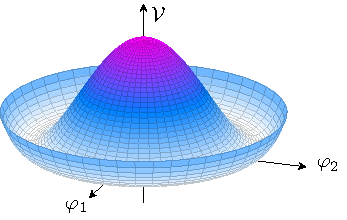
\includegraphics[width=0.6\textwidth]{figurer/mexican_hat.pdf}
    \caption{The Mexican hat potential is the classical potential $\Ve$ for the $N=3$ linear sigma model.}
    \label{fig:Mexican hat}
\end{figure}

\subsection*{Lie groups}

Lie groups are a natural structure to capture the symmetries of a theory.
A Lie group is a smooth manifold, i.e. a space that is locally diffeomorphic to $\R^N$.
This means that we can locally parametrize the space by $N$ real numbers $\eta_\alpha$, using smooth invertible functions.
A Lie group is also equipped with group structure.
A group is a set, $G$, together with a map
\begin{align}
    (\cdot, \cdot):  G \times G &\longmapsto G ,\\
    (g_1, g_2) &\longmapsto g_3,
\end{align} 
called group multiplication. This map obeys the group axioms, which are the existence of an identity element $\one$, associativity and the existence of an inverse element $g^{-1}$ for all $g\in G$.
These can be written as
\begin{align*}
    (g, \one) &= g, \\
    (g_1, (g_2, g_3)) &= ((g_1, g_2), g_3), \\
    (g, g^{-1}) &= \one.
\end{align*}
In addition, we require that both the multiplication map and the inverse map, $g \mapsto g^{-1}$ are smooth.
We describe the set of continuous symmetry transformations, 
\begin{equation}
    G = \setbuilder{g}{g \varphi = \varphi', \, S[\varphi'] = S[\varphi], \D \varphi' = \D \varphi },
\end{equation}
as a Lie group, where the group multiplication is composition, i.e. performing transformations in succession.
This map is closed, as two symmetry transformations are another transformation.
The identity map is a symmetry transformation, and composition is associative.
This means that invertible symmetry transformations form a group.

We will focus on connected Lie groups, in which we all elements $g \in G$ is in the same connected piece as the identity map $\one \varphi = \varphi$.
This means that for each $g\in G$, one can find a continuous path $\gamma(t)$ in the manifold, such that $\gamma(0) = \one$ and $\gamma(1) = g$.
Given such a path, we can study transformations close to the identity.
As the Lie group is a smooth manifold, we can write\footnote{The factor $i$ is a physics convention, and differs from how mathematicians define generators of a lie group.}
\begin{equation}
    \gamma(\epsilon) = \one + i \epsilon V + \Oh{\epsilon}
\end{equation}
$V$ is a generator, and can be defined as
\begin{equation}
    iV = \diff{\gamma}{t}\Big|_{t=0}.
\end{equation}
We can define a path $\gamma$ by its path through parameter space, $\gamma(t) = g(\eta(t))$, which means that we can write the generator as
\begin{equation}
    V = \diff{\gamma}{t}\Big|_{t=0} = \diff{\eta_a}{t}\Big|_{t=0} \diffp{g}{\eta_a}\Big|_{\eta=0}
    = \diffp{g}{\eta_a}\Big|_{\eta=0} T_\alpha, \quad 
    T_\alpha = \diffp{g}{\eta_\alpha}.
\end{equation}
We see that the generators form a vector space, with the basis $T_\alpha$, induced by the coordinates $\eta_a$.
This vector space is called the tangent space of the identity element, $T_\one G$.
Infinitesimal transformations can therefore be written as
\begin{equation}
    \gamma(\epsilon) = \one + i \epsilon v_\alpha T_\alpha, \quad \epsilon \rightarrow 0.
\end{equation}
The tangent space, together with the additional operation
\begin{align}
    [T_\alpha, T_\beta] = iC_{\alpha\beta}^\gamma T_\gamma,
\end{align}
called the Lie bracket, forms a Lie algebra denoted $\mathfrak{g}$.
For matrix groups, which are what we deal with in this text, the Lie bracket is the commutator.
$C_{\alpha \beta}^\gamma$ are called structure constants.
They obey the Jacobi identity,
\begin{equation}
    \label{jacobi identity}
    C_{\alpha \beta}^\gamma + C_{\beta\gamma}^\alpha +  C_{\gamma\alpha}^\beta = 0,
\end{equation}
which mean that they are totally antisymmetric.
A subset of the original Lie group, $H \subset G$, which is closed under the group action is called a subgroup.
$H$ then has its own Lie algebra $\mathfrak{h}$, with a set of $m = \dim H$ generators, $x_i$, which is a subset of the original generators $T_\alpha$
We denote the remaining set of generators $t_a$, such that $x_i$ and $t_a$ together span $\mathfrak{g}$.

Of special importance are one parameter subgroups.
If a curve $\gamma(t)$ through $G$ obey
\begin{equation}
    \gamma(t)\gamma(s) = \gamma(t + s), \quad \gamma(0) = \one,
\end{equation}
then all the points on this curve from a one parameter subgroup of $G$.
This path is associated with a generator, 
\begin{equation}
    \diff{\gamma}{t} \Big|_{t=0} = i \eta_\alpha T_\alpha.
\end{equation}
This allows us to define the exponential map,
\begin{equation}
    \exp{i \eta_\alpha T_\alpha} := \gamma(1).
\end{equation}
For connected and compact Lie groups, all elements of the Lie group $g \in G$ can be written as an exponential of elements in the corresponding Lie algebra $\eta_\alpha T_\alpha \in \mathfrak g$.
For matrix groups, the exponential equals the familiar series expansion
\begin{equation}
    \exp{X} = \sum_n \frac{1}{n!} X^n.
\end{equation}

A subgroup $H \in G$ has its own Lie algebra $\mathfrak{h}$, with a set of $m = \dim H$ generators, $x_i$, which is a subset of the original generators $T_\alpha$.
We denote the remaining set of generators $t_a$, such that $x_i$ and $t_a$ together span $\mathfrak{g}$.
The commutators of $x_i$ must be closed, which means that we can write
\begin{align}
    [x_i, x_j] &= i C_{i j}^{k} x_k,\\
    [x_i, t_a] &= i C_{i a}^b t_b, \\
    [t_a, t_b] &= i C_{ab}^k x_k + i C_{ab}^c t_c,
\end{align}
where $ijk$ runs over the generators of $\mathfrak h$, and $abc$ runs over the rest.
The second formula can be derived using the Jacobi identity \cref{jacobi identity}, which implies that $C_{ia}^k = -C_{ik}^a = 0$.
This is called a Cartan decomposition.

\subsection*{Goldstone's theorem}

The fact that a theory is left invariant under some symmetry transformation does not imply that the ground state is invariant under this transformation.
The $N = 2$ linear sigma model illustrates this.
If we assume the ground state $\varphi_{0}$ is translationally invariant, then it is given by minimizing the effective potential, of which the classical potential, $\Ve$, is the leading order approximation.
This potential is illustrated in \autoref{fig:Mexican hat}.
The ground state is therefore given by any of the values along the brim of the potential.
If we, without loss of generality, choose $\varphi_0 = (0, v)$ as the ground state, then any symmetry transformation will change this state.
We say that the symmetry has been \emph{spontaneously broken}.

To explore this in a general context, assume a theory of $\varphi_i$ real scalar fields are invariant under the actions of some Lie group, $G$.
A symmetry $g \in G$ is broken if the vacuum expectation value of the original fields and the transformed fields differ.
That is, if
\begin{equation}
    \ex{\varphi}_0 \neq \ex{\varphi'}_0 = \ex{g \varphi}_0
\end{equation}
We can now exploit what we learned about Lie groups to write
\begin{equation}
    \ex{\varphi'}_0 = \ex{\varphi}_0 + i \epsilon \eta_\alpha T_\alpha \ex{\varphi}_0.
\end{equation}
Let $t_a$ be the set of generators corresponding to broken symmetries, i.e.
\begin{equation}
    t_\alpha \ex{\varphi}_0 \neq 0.
\end{equation}
These are called the \emph{broken generators}.
The remaining set of generators $x_i$, which obey
\begin{equation}
    x_i \ex{\varphi}_0 = 0,
\end{equation}
are called unbroken, and generate a subgroup $H \subset G$ as the set of symmetry transformations of the vacuum is a group.

In \cref{effective equation of motion} we found that the effective action obey
\begin{equation}
    \int \dd^4 x \fdiff{\Gamma[\varphi_J]}{\varphi_i} t_{ij} \ex{\varphi_j}_0 = 0.
\end{equation}
We now differentiate this expression with respect to $\varphi_k(y)$ and evaluate it in the vacuum, which gives
\begin{equation}
    \int \dd^4 x \, \fdiff{\Gamma[\varphi_0]}{\varphi_k(y), \varphi_i(x)}
    t_{ij} \ex{\varphi_j}_0 = 0.
\end{equation}
With the assumption that the ground state is constant, we get 
\begin{equation}
    \diffp{\Veff}{\varphi_k, \varphi_i} \, t_{i j} \ex{\varphi_j}_0 = 0.
\end{equation}
This is trival for unbroken symmetries, as $t_{ij}\ex{\varphi_j}_0 = 0$ by definition.
However, in the case of a broken symmetry, the second derivative of the effective potentail has an eigenvector $t^\alpha_{ij} \ex{\varphi_j}$ with a zero eigenvalue for each broken generator.
In \autoref{Effective action inverse propagator}, we found that the second derivative of the effective action is the inverse propagator,
\begin{equation}
    D^{-1}_{ij}(x,y) 
    = -i \fdiff{\Gamma[\varphi_0]}{\varphi_i(y), \varphi_j(x)}
    = \int \frac{\dd^4 p}{(2 \pi)^4} e^{-ip(x - y)} \, \tilde D^{-1}_{ij}(p).
\end{equation}
Using this, we can write
\begin{equation}
    \tilde D^{-1}_{i j}(p=0) \, t^\alpha_{j k} \ex{\varphi_k}_0 
    = 0.
\end{equation}
Zeros of the inverse propagator corresponds to the physical mass of particles.
In Lorentz-invariant systems, each zero-mass vector corresponds to a masses particles, called a Goldstone boson.\footnote{ The particles are bosons due to the bosonic nature of the transformations, $t$. If the generators are Grassmann numbers, the resulting particle, called a goldstinos, are fermions.}
This means there are $n_G = \dim G -\dim H$ zero mass modes.
In general, counting of massless modes is more complicated, and depends on the dispersion relation of the particles at low momenta.
Systems with Goldstone bosons with quadratic dispersion relation, that is $E = |\vv p|^2$ when $\vv p \rightarrow 0$, often exhibit a lower number of massless modes.
An example is ferromagnets, where the $\mathrm{SU}(2)$ rotational symmetry is broken down to $\mathrm{U}(1)$ when they align along one axis. 
This corresponds to two broken generators, yet the system only exhibits one massless mode~\cite{brauner_spont_sym}.

\begin{figure}[ht]
    \centering
    \begin{subfigure}{0.54\textwidth}
        \centering\captionsetup{width=.9\linewidth}
        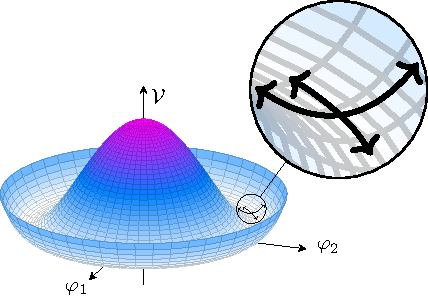
\includegraphics[]{figurer/mexican_hat_zoom.pdf}
        \caption{Excitations along the brim does not cost any energy, as the potential is flat, unlike excitations in the radial direction.}
        \label{fig:Mexican hat zoom}
    \end{subfigure}
    \begin{subfigure}{0.45\textwidth}
        \centering\captionsetup{width=.9\linewidth}
        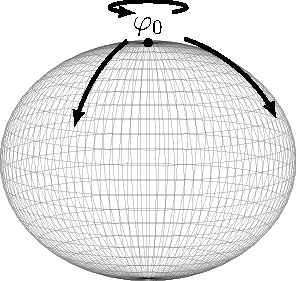
\includegraphics[]{figurer/sigma_ground_state.pdf}
        \caption{Excitations for the $N=3$ sigma model. Two of the symmetries are broken, while rotations around the groundstate leaves the system unchanged.}
        \label{fig:ground state manifold}
    \end{subfigure}
\end{figure}

The linear sigma model gives an intuition for the Goldstone mode.
In the case of $N = 2$, the symmetry of the Lagrangian are rotations in the plane.
As the ground state is a point along the ``brim'' of the hat, this rotational symmetry is broken.
Any excitations in the rotational direction, however, does not cost any energy, which is indicative of a massless mode.
This is illustrated in \autoref{fig:Mexican hat zoom}.
In this example, the original symmetry group is one dimensional, so there are no unbroken symmetries.
If we instead consider the $N=3$ linear sigma model, which has a three-dimensional symmetry group, rotations of the sphere, we see that the ground state is left invariant under subgroup of the original symmetry transformations.
The ground state manifold of this system, the set of all states that minimizes the effective potential, is then a sphere.
When the system chooses one single ground state, this symmetry is broken, but only for two of the generators. 
The generator for rotations around the ground state leaves the that point unchanged, and is thus an unbroken symmetry.
Any excitations in the direction of the broken symmetries does not cost energy, as it is in the ground state manifold.
The unbroken symmetry, on the other hand, does not correspond to an excitation.
This is illustrated in \autoref{fig:ground state manifold}.


\section{CCWZ construction}
\label{seciton:ccwz construction}

As Goldstone bosons are massless, they play a crucial role in the low energy dynamics.
To best describe this limit, we seek a parametrization of the fields in which they are the degrees of freedom.
This can be done using the CCWZ construction, named after Callan, Coleman, Wess and Zumino.
As well as the original papers~\cite{Structure_of_phen_1,Structure_of_phen_2}, this section is based on~\cite{weinberg_1996_vol2,The_composite_NG_Higgs,effective_FT_with_NG_modes} and\footnote{\url{http://scipp.ucsc.edu/~haber/archives/physics251_17/PHYS251_Presentation_L_Morrison}}. (REFERER ORDENTLIG)


We saw that the Goldstone bosons corresponds to excitations within the vacuum manifold.
The vacuum manifold corresponds to points in field space $\varphi$ that can be reach from the vacuum $\varphi_0$ with a transformation $g \in G$.
This means that we can write such excitations as
\begin{equation}
    \varphi = \tilde\Sigma \varphi_0, \quad \tilde \Sigma = \tilde \Sigma(\eta) = \exp{i \eta_\alpha T_\alpha}
\end{equation}
$\tilde \Sigma$ is thus a function from the parameter space, $\eta_\alpha \in \R^n$ to $G$,
\begin{align}
    \tilde \Sigma: \R^n \longmapsto G.
\end{align}
We then get space-time dependent field configurations by making the parameters dependent on spacetime.
We will for now assume $\eta_\alpha$ is constant.
%TODO: Forklar hvorfor vi ikke bryr oss
% $\varphi(x)$ is not a completely generic field configurations, as it does not account for fluctuations in directions other than those in $G$, but we don't care. (?)
This parametrization is highly redundant.
There are $n = \dim G$ parameters $\eta$, but Goldstone's theorem says that there is one massless mode per broken generator.
Two elements $\tilde\Sigma$ and $\tilde\Sigma'$, related by
\begin{equation}
    \tilde \Sigma' = \tilde\Sigma e^{i \theta_a t_a}
\end{equation}
results in the same $\varphi$.
This is because  $e^{i \theta_a t_a} = h \in H$, and $h \varphi_0 = \varphi_0$, by assumption.
The set of all equivalent $\tilde \Sigma$'s is exactly the left coset, $gH = \setbuilder{gh}{ h \in H}$.
The set of cosets forms a new manifold, $G / H$, called the Goldstone manifold.
This is a manifold of dimension $\dim(G/H) = \dim(G) - \dim(H)$, which is exactly the number of broken generators, and thus also the number of Goldstone modes.
Membership of a certain coset from an equivalence relation, $g \sim g'$ if $g' = gh$.
This means that the cosets $gH$ form a partition of $G$, and that each element $g \in G$ belongs to one, and only one, coset.
To remove the redundancy in the parametrization, we need to choose one representative element from each coset.

By the inverse function theorem, any mapping between manifolds $f: \Em \mapsto \mathcal{N}$ that has a non-degenerate differential, that is an invertible Jacobian, at a point $p \in \Em$, is invertible in a neighborhood of $p$.
The map
\begin{equation}
    \tilde \Sigma(\xi, \theta) = \exp{i \xi_i x_i} \exp{i \theta_a t_a}
\end{equation}
is invertible at $p = (\xi_i = 0, \theta_a = 0)$, which is mapped to the identity, as the Jacobian is the identity matrix.
This means that, in a neighborhood $U \subset G$ of the identity, each element $g$ has a unique representation $g = \Sigma$~\cite{smooth_manifolds}.
Furthermore, two elements $\tilde \Sigma'$ and $\tilde \Sigma$ related by $\tilde \Sigma' = \tilde \Sigma h$, $h \in H$ have the same $\xi$-arguments.
We see that $\xi_i$ parametrize $G/H$, in the neighborhood of the identity.
We therefore demand that $\tilde \Sigma$ always appear in the standard form
\begin{equation}
    \Sigma(\xi) = \tilde \Sigma(\xi, 0) = \exp{i \xi_i x_i}.
\end{equation}
The field $\varphi(x)$ can therefore be written as
\begin{equation}
    \varphi(x) = \Sigma(x) \varphi_0 = \exp{i \xi_i(x) x_i} \varphi_0,
\end{equation}
and $\xi_i(x)$ can be associated with the Goldstone bosons.

In the linear sigma model, the original $O(N)$ symmetry is broken down to $O(N-1)$, which transforms the remaining $N-1$ fields with vanishing expectation value into each other.
However, $O(N)$ consists of two disconnected subsets, those matrices with determinant 1 and those with determinant -1.
There is no continuous path that takes an element of $O(N)$ with determinant of $-1$ to an element with determinant 1.\footnote{A simple proof of this is the fact that the determinant is a continuous function, while any path $\det M(t)$ such that $\det M(1) = -1,\, \det m(0) = 1$ must make a discontinuous jump.}
The set of symmetries that are connected to the identity is
\begin{eqnarray}
    G = SO(N) = \setbuilder{M \in O(N)}{ \det M = 1}.
\end{eqnarray}
If we choose $\varphi_0 = (0, 0, ..., v)$, then it is apparent that the ground state is invariant under the rotations of the $N-1$ first fields, so the unbroken symmetry is  $H = SO(N-1)$.
The Goldstone manifold is $G/H = SO(N) / SO(N-1)$.

Consider the case of $N = 3$, which is illustrated in \autoref{fig:ground state manifold}.
$G$ is the rotations of the sphere, while $H$ is rotations around $\varphi_0$, $SO(2)$.
The Goldstone manifold consists of the rotations of $\varphi_0$ to other points of the sphere, i.e. $G/H = SO(3)/S(2) = S^2$, the 2-sphere.
This is not a Lie group, as translating $\varphi$ in a closed path around the sphere may result in a rotation around the z-axis.


To check that $\xi_i$ in fact are the Goldstone modes, we study the way they appear in the Lagrangian.
As they are massless, no mass term of the form $M_{ij} \xi_i \xi_j$ should appear in the Lagrangian.
The original Lagrangian $\Ell[\varphi]$ was invariant under global transformations $\varphi(x) \mapsto g \varphi(x)$.
However, any terms that only depend on $\varphi(x)$, and not its derivatives, will also be invariant under a \emph{local} transformation, $\varphi(x) \mapsto g(x)\varphi(x)$.
Our parametrization of the fields, $\varphi(x) = \Sigma(x)\varphi_0$ is exactly such a transformation, which means that any such terms are independent of the Goldstone bosons.
We can therefore write
\begin{equation}
    \Ell[\varphi] = \Ell_{\mathrm{kin}}[\varphi] + V(\varphi_0),
\end{equation}
where all terms in $\Ell_{\mathrm{kin}}$ are proportional to at least one derivative term, $\partial_\mu \varphi(x)$.
Inserting the parametrization into this derivative term, we get
\begin{equation}
    \partial_\mu \varphi(x) = \partial_\mu [\Sigma(x) \varphi_0]
    = \Sigma(x) [\Sigma(x)^{-1} \partial_{\mu} \Sigma(x)] \varphi_0.
\end{equation}
The Lagrangian will therefore depend on $\xi_i$ via terms of the term $\Sigma(x)^{-1}\partial_\mu \Sigma(x)$, which is called the Mauer-Cartan form.
This is a $\mathfrak g$-valued function, which means that it can be written on the for
\begin{align*}
    i\Sigma(x)^{-1}\partial_\mu \Sigma(x) & 
    = d_{\mu}(x) + e_{\mu}(x), \\
    d_{\mu} & = i x_i d_{ij}(\xi) \partial_\mu \xi_j, \\
    e_{\mu} & = i t_a e_{ai}(\xi)\partial_\mu \xi_i,
\end{align*}
where $d_{ij}$ and $d_{ai}$ are as-of-yet unknown real valued functions of $\xi$~\cite{weinberg_1996_vol2,Watanabe:effective_lagrangian}.

\subsection*{Transformation properties of Goldstone bosons}
We can deduce how the Goldstone bosons transforms under $G$ from how $\varphi$ transforms.
In general, 
\begin{equation}
    \varphi' = g \varphi = (g \Sigma(\xi)) \varphi_0 = \Sigma(\xi') \varphi_0 \quad g \in G.
\end{equation}
While $\Sigma(\xi')$ has the standard form by assumption,
\begin{equation}
    \Sigma(\xi') = \exp{i \xi'_i x_i},
\end{equation}
$g\Sigma(\xi)$ does not, in general.

\begin{figure}[h]
    \centering
    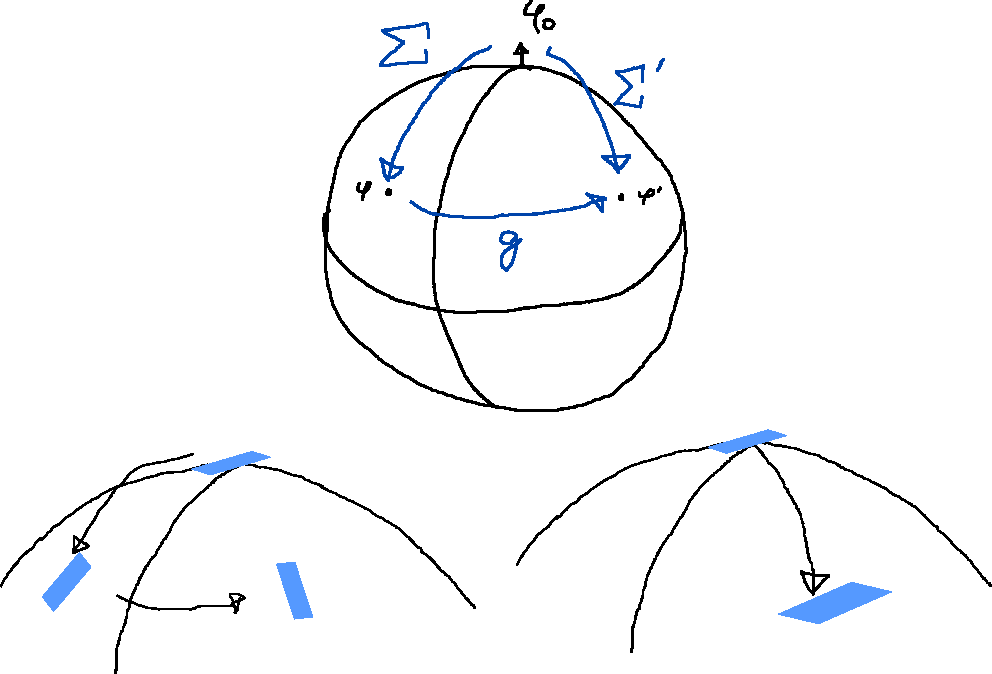
\includegraphics[width=0.8\textwidth]{figurer/parallel_transport_kladd.pdf}
    \caption{(KLADD) The top figure illustrates the transformation of $\varphi_0$ to $\varphi$ and then $\varphi$, and the alternative transformation $\varphi_0 \rightarrow \varphi'$. The bottom figure illustrates how this can rotate a neighborhood of $\varphi_0$ differently.}
    \label{fig:Curvature of SO(3)}
\end{figure}
\autoref{fig:Curvature of SO(3)} illustrates this in the case of $G = SO(3)$.
$\Sigma(\xi)$ transforms $\varphi_0$ to $\varphi$, then $g$ transforms $\varphi$ to $\varphi' = \Sigma(\xi') \varphi_0$.
Assuming $\varphi$ and $\varphi'$ are close enough to $\varphi_0$, we can write $\Sigma(\xi)$ and $\Sigma(\xi')$ on the standard form.
However, if we follow a small neighborhood around $\varphi_0$ as it is acted on by $\Sigma(\xi)$, then $g$, it will be rotated by the time it arrives at $\varphi'$, when compared to the same neighborhood if it was acted on by $\Sigma(\xi')$.

$g\Sigma(\xi)$ and $\Sigma(\xi')$ are in the same coset, as they by assumption corresponds to the same physical state.
This means that we can write $g\Sigma(\xi) = \Sigma(\xi') h(g, \xi)$, where $h(g, \xi) \in H$.
The transformation rule of $\xi$ under $G$ is therefore implicitly defined by
\begin{equation}
    \Sigma(\xi') = g \Sigma(\xi) [h(g, \xi)]^{-1}.
\end{equation}
This is in general not a linear representation, which is why this construction also is called a \emph{non-linear realization}.
Using the transformation rule, we can obtain the transformation rule of the Maurer-Cartan form.
We use the shorthand $\Sigma = \Sigma(\xi),\, \Sigma' = \Sigma(\xi')$, and $h = h(g, \xi)$.
This gives
\begin{align*}
    \Sigma^{-1} \partial_\mu \Sigma
    \rightarrow 
    & \, \Sigma'^{-1} \partial_\mu \Sigma' \\
    & = (g \Sigma h^{-1})^{-1} \partial_\mu (g \Sigma h^{-1}) \\
    & = (h \Sigma^{-1} g^{-1}) g [(\partial_\mu \Sigma)h^{-1} + \Sigma \partial_\mu h^{-1}] \\
    & = h \Sigma^{-1} (\partial_\mu \Sigma) h^{-1}
    + h \partial_\mu h^{-1} \\
    & = h (\Sigma^{-1} \partial_\mu \Sigma + \partial_\mu) h^{-1}.
\end{align*}
In terms of $d_\mu$ and $e_\mu$,
\begin{align}
    d_\mu & \rightarrow h d_\mu h^{-1} \\
    e_\mu & \rightarrow h (e_\mu + i\partial_\mu )h^{-1}.
\end{align}
These are our building blocks for constructing a general, $G$-invariant effective Lagrangian.
The trace of a product of $d_\mu$'s are invariant under $G$,
\begin{equation}
    \Tr{d_\mu d_\nu \dots d_\rho} 
    \rightarrow
    \Tr{h d_\mu h^{-1} h d_\nu h^{-1} h \dots d_\rho h^{-1}}
    = \Tr{d_\mu d_\nu \dots d_\rho},
\end{equation}
where we have used the cyclic property of trace.
However, the terms must also obey the other symmetries of the Lagrangian, such as C or P-parity and Lorentz invariance.
The last criterion excludes any terms with free spacetime indices.
In \autoref{section:chiral pertubation theory}, we will construct an effective Lagrangian in powers of $d$.
The lowest order terms are therefore
\begin{equation}
    \label{first order terms CCWZ}
    \Tr{d_\mu} \Tr{d^\mu}, 
    \quad 
    \Tr{d_\mu d^\mu}.
\end{equation}
We see that $e_\mu$ transforms like a gauge field, with the gauge group $H$.
If we include massive degrees of freedom, and not only the boson modes, $e_\mu$ is used to create a covariant derivative of the massive modes.
We are only interested in the Goldstone, and will therefore be satisfied with $d_\mu$.
With these tools, we can create an effective theory of quantum chromodynamics at low energies.

% (KANSKJE?: Inkluder massiver partikler, med $\varphi(x) = \Sigma(x)\tilde \varphi(x)$, og hvordan det transformerer. Skriver om representasjoner? (adj, r pi))


% % Effective Lagrangian
\chapter{The effective theory of pions}
\label{chapter:effective theory of pions}

\section{QCD}

In this paper we consider an effective theory of quantum chromo dynamics, QCD, at low temperature and with two quarks, up and down.
These quarks has a mass matrix 
\begin{equation}
    \label{Mass matrix}
    M =
    \begin{pmatrix}
        m_u & 0 \\
        0 & m_d
    \end{pmatrix}.
\end{equation}
In the isospin limit, $m_u = m_d$, the theory is invariant under global transformations by elements of the group $G' = \lieg{SU}{2}_L \times \lieg{SU}{2}_R \times \lieg{U}{1}_V$.
All terms involving only pions are trivially invariant under $\lieg{U}{1}_V$, (HVORFOR?) so we focus on the $G = \lieg{SU}{2}_L \times \lieg{SU}{2}_R$ subgroup.

(TODO: SKRIVE OM DE RELEVANTE EGENSKAPENE TIL QCD)
\section{Chiral perturbation theory}
\label{section:chiral pertubation theory}
This section is base on \cite{Schwartz:QFT,weinberg_1996_vol2,Scherer2002IntroductionTC}, in addition to the original work~\cite{Gasser-Leutwyler:chiral,WeinbergPhenom,Scherer:PhysRevD.53.315}

In this paper, we will consider the interaction of the two lightest quarks, the up and down quarks $u$ and $d$, i.e. $N_f = 2$.
In this case, the symmetry group of rotations in the flavor indices are $G_f = U(1) \times \SU(2)_L \times \SU(2)_R$.
The generators of $\SU(2)$ are $T_\alpha = \tau_\alpha / 2$, where $\tau_\alpha$ are the Pauli matrices, as described in \autoref{section:algebra bases}.
The mass matrix of the quarks is
\begin{equation}
    \label{Mass matrix}
    m =
    \begin{pmatrix}
        m_u & 0 \\
        0 & m_d
    \end{pmatrix}
    = \frac{1}{2} (m_u + m_d) \one + \frac{1}{2}(m_u - m_d) \tau_3,
\end{equation}
where $m_u \approx 2.16 \, \text{MeV}$, and $m_d \approx 4.67 \, \text{MeV}$~\cite{PDG}.
This means that the $G_f$ symmetry is \emph{explicitly} broken.
% In last section, we saw that for $m_u = m_d$, the subgroup $U(1) \times \SU(2)_V$ remains intact.
% This is called the isospin-limit.
% However, as $m_u \neq m_d$, also the isospin subgroup $\SU(2)_V$ is broken.
% The difference between these masses is small, which is why isospin is a good quantum number.
Even though the underlying symmetry is only approximate, we can still apply the formalism from Goldstone's theorem and the CCWZ construction by including a small mass term for the Goldstone bosons, which in this case are called \emph{Pseudo Goldstone bosons}.

We now focus on the subgroup $G = \SU(2)_L \times \SU(2)_R$.
The ground state spontaneously breaks this approximate symmetry of the two-flavor QCD Lagrangian.
As quarks $q$ are spinors, a non-zero expectation value of the quark field would break Lorentz-invariance.
Instead, the spontaneous symmetry breaking is characterized by the \emph{scalar quark condensate}, $\ex{\bar q q}$.
The scalar quantity $\bar q q$ is invariant under isospin transformations $H = \SU(2)_V$, but not under $\SU(2)_A$.
The Goldstone manifold, therefore, is $G/H = \SU(2)_L\times \SU(2)_R/\SU(2)_V = \SU(2)_A$.
To model the low-energy dynamics of QCD, we start with the massless QCD Lagrangian,
\begin{align*}
    \Ell^0_\mathrm{QCD}[q, \bar q, A_\mu] 
    = i \bar q \slashed{D} q - \frac{1}{4}G_{\mu \nu}^\alpha G^{\mu \nu}_\alpha.
\end{align*}
Following~\cite{Scherer2002IntroductionTC,Gasser-Leutwyler:chiral}, we couple quarks to external currents.
These can be used to model external fields or capture the symmetry-breaking mass term.
As found in \autoref{section:QCD}, the conserved currents are
\begin{equation}
    V_a^\mu = \frac{1}{2} \bar q \gamma^\mu \tau_a q, \quad
    A_a^\mu = \frac{1}{2} \bar q \gamma^\mu \gamma^5 \tau_a q, \quad
    J^\mu = \bar q \gamma^\mu q.
\end{equation}
In addition, external currents can couple to the scalar and pseudo-scalar quark bilinears
\begin{equation}
    \bar q q, \quad \bar q \gamma^5 q, 
    \quad \bar q \tau_a q, \quad \bar q \gamma^5 \tau_a q.
\end{equation}
The Lagrangian of the external is
\begin{align}
    \Ell_\text{ext} 
    & = 
    - (\bar q q )\, s_0 + (i \bar q \gamma^5 q) \, p_0
    - (\bar q \tau_a q)\, s_a + (i \bar q \gamma^5 \tau_a q) \, p_a
    + \frac{1}{3} J_\mu v_{(s)}^\mu 
    + V_\mu^a v_a^\mu + A_\mu^a a_a^\mu \\
    & = 
    - \bar q \left(s + i \gamma^5 p \right) q
    + \bar q \left(\frac{1}{3} v^\mu_{(s)} + v^\mu + a^\mu \gamma^5\right) \gamma_\mu q.
\end{align}
Here, $v, v_{(s)}, a, s$ and $p$ are the external source currents, where we denote
\begin{equation}
    s = s_0 \one + s_a \tau_a, \quad
    p = p_0 \one + p_a \tau_a, \quad
    v^\mu = \frac{1}{2} v_a^\mu \tau_a, \quad
    a^\mu = \frac{1}{2} a_a^\mu \tau_a.
\end{equation}
Setting $v = v_{(s)} = a = s = p = 0$, we recover the chiral limit.
To include the effect of the quark masses, we set $s = m$.
We denote all the external currents as $j = (v, v_{(s)}, a, s, p )$.
As with the conserved currents, we define
\begin{equation}
    v_\mu = \frac{1}{2}(r_\mu + l_\mu),
    \quad
    a_\mu = \frac{1}{2}(r_\mu - l_\mu).
\end{equation}
With this, as well as 
\begin{equation}
    \bar q (s - i \gamma^5 p) q
    = \bar q_R (s - i p) q_L + \bar q_L (s + i p) q_R,
\end{equation}
we can write the Lagrangian as
\begin{equation}
    \Ell_\text{ext} 
    = - \bar q_R (s + i p) q_L - \bar q_L (s - i p) q_R
    + \frac{1}{3} (J_R^\mu + J_V^\mu)(v_{(s)})_\mu
    + R_\mu^a r^\mu_a + L_\mu^a l^\mu_a
\end{equation}
The generating functional is then
\begin{equation}
    Z[j] 
    = 
    \int \D \bar q \D q \D A_\mu \, 
    \exp{
        i \int \dd^4 x 
        \left( 
            \Ell^0_\text{QCD}[q, \bar q, A_\mu] + \Ell_\text{ext}[q, \bar q, j]
        \right)
    }
\end{equation}
We will now use the CCWZ construction and effective field theory to construct the effective Lagrangian, which obeys
\begin{equation}
    Z[j] = \int \D \pi \, \exp{i \int \dd^4 x \, \Ell_\text{eff}[\pi]},
\end{equation}
where $\pi$ are the Goldstone bosons.

\subsection*{Weinberg's power counting scheme}
\label{subsection:power counting}

We now have a relationship between the underlying Lagrangian and the effective Lagrangian, of the form \autoref{integrating out degrees of freedom}.
However, as discussed earlier, we cannot solve QCD at low energies and thus have no way to integrate out the high energy degrees of freedom.
Instead, we have to make use of Weinberg's ``theorem''.
Using the CCWZ construction, we can obtain the most general Lagrangian obeying the symmetries of QCD. 
In this case, we have not laid any constraints on the theory but the most basic assumptions.
This, however, will result in a theory with an infinite number of free parameters, making it rather unwieldy.
To amend this, we need a scheme to order the terms to compute observable perturbatively.
We are working in the low-energy regime, so it is natural to expand in pion momenta.
As we saw in \autoref{seciton:ccwz construction}, the terms in the Lagrangian will be made up of combinations of the terms $e_\mu$ and $d_\mu$ of the Maurer-Cartan form, $i\Sigma \partial_\mu \Sigma = e_\mu + d_\mu$.
Therefore, all terms in the effective Lagrangian will be proportional to a certain number of derivatives, which Lorentz invariance demands to be even.

Consider the matrix element $\mathcal M$ for a given Feynman diagram with external pion lines with momenta $q_n$, where both the energies and momenta are less or equal to some energy scale $Q$.
If we scale $Q\rightarrow tQ$, and consequently also the external momenta $q_n \rightarrow tq_n$, momentum conservation at each vertex ensures that each internal momentum $p$ of the diagram scales as $p \rightarrow tp$.
Assume this diagram is made up of $V_i$ copies of the vertex $i$, which contain $d_i$ derivatives.
Each of these vertices then scale as $t^{d_i}$.
The propagators contribute a factor $p^{-2}$ and will therefore scale as $t^{-2}$, and the integration measure $\dd^4 p$ scales as $t^4$.
This means that a matrix element with $L$ loops and $I$ internal lines scales as
\begin{equation}
    \mathcal M(q) \rightarrow \mathcal M(t q) = t^D \mathcal M(q),
\end{equation}
where 
\begin{equation}
    D = \sum_i V_i d_i - 2 I + 4 L.
\end{equation}

$D$ is called the \emph{chiral dimension} of $\mathcal M$.
Using the formula \cref{Number of loops} for number of loops in a Feynman diagram, we get
\begin{equation}
    D = \sum_i V_i(d_i - 2) + 2 L + 2.
\end{equation}
For low energy scales $Q$, the larges contribution will come from the matrix elements of the smallest chiral dimension $D$.
A general process will consist of a sum of matrix elements of different chiral dimensions.
We can expand this element in powers of the pion momenta by using $t$ as the expansion parameter.
The leading order term will be those where $L = 0$ and $d_i = 2$ so that $D = 2$.
This means that all tree-level contributions to lowest chiral dimension are from terms in the Lagrangian with exactly two derivatives.
Next is $D = 4$, which contains both tree-level contributions from terms with $d_i = 4$ and a one-loop contribution from $d_i = 2$.
We therefore expand the effective Lagrangian as
\begin{equation}
    \Ell_\text{eff} = \Ell_2 + \Ell_4 + ...,
\end{equation}
where $\Ell_{2n}$ contains $2n$ derivatives.
This is equivalent to scaling the space-time cooridnates as $x^\mu \rightarrow tx^\mu$, and expanding the Lagrangian in powers of $t$.

We must also allow for the fact that pions have non-zero mass and that there is a finite isospin chemical potential.
This is all implemented by external currents, which we also have to assume are small.
Any external pions are on-shell, so the pion mass $m_\pi$ must be less than the energy scale $Q$.
As we will see, this corresponds to scaling the quark masses as $m_q \rightarrow t^2 m_q$.
Similarly, $\mu_I$ must also be less than $Q$, which means that we scale it as $\mu_I\rightarrow t \mu_I$.
Following these rules, each term in the effective Lagrangian will have a well-defined chiral dimension $D$, ensuring a consistent series expansion.
The term $\Ell_{D}$ then contain all allowed terms that scale as $t^D$~\cite{weinberg_1996_vol2,WeinbergPhenom,Scherer2002IntroductionTC}.

\subsection*{Non-linear realization}

To parametrize the low energy behavior of QCD, we must find a representative element of the coset space of $G$, $G/H = \SU(2)_A$.
Let $g\in G$. 
We write $g = (U_L, U_R)$, where $U_R \in \SU(2)_R$, $U_L \in \SU(2)_L$.
Elements $h \in H$ are then of the form $h = (U, U)$.
A general element g can be written as
\begin{equation}
    g = (U_L, U_R) = (1, U_R U_L^\dagger) (U_L, U_L).
\end{equation}
Since $(U_L, U_L) \in H$, this means that we can write the coset $g H$ as $(1, U_R U_L^\dagger)H$, which gives a way to choose a representative element for each coset.
We identify
\begin{equation}
    \Sigma = U_R U_L^\dagger. 
\end{equation}
This is our standard form for elements in $gH$.
As we saw in \autoref{seciton:ccwz construction}, it therefore implicitly define transformation properties of the Goldstone bosons, which is given by the function $h(g, \xi)$.
For $\tilde g \in G$, we have 
\begin{equation}
    \tilde g (1, \Sigma)
    = (\tilde U_L, \tilde U_R) (1, U_R U_L^\dagger)
    = (1, \tilde U_R (U_R U_L^\dagger) \tilde U_L^\dagger) (\tilde U_L, \tilde U_L)
    = (1, \tilde U_R \Sigma \tilde U_L) \tilde h.
\end{equation}
This gives the transformation rule
\begin{equation}
    \Sigma \rightarrow \Sigma' = U_R \Sigma U_L^\dagger.
\end{equation}
Under transformations by $h = (U, U^\dagger) \in H$, we have
\begin{equation}
    \label{sigma transform under H}
    \Sigma \rightarrow \Sigma' = U \Sigma U^\dagger.
\end{equation}
As $\partial_\mu  (1, \Sigma) = (0, \partial_\mu \Sigma)$, the constituents of the Mauer-Cartan form are
\begin{equation}
    d_\mu = i \Sigma(x)^\dagger \partial_\mu \Sigma(x),\quad
    e_\mu = 0.
\end{equation}
Using $\partial_\mu [\Sigma(x)^\dagger\Sigma(x)] = 0 $, we can write
\begin{equation}
    d_\mu d^\mu = 
    - \Sigma(x)^\dagger [\partial_\mu \Sigma(x)] \Sigma(x)^\dagger [\partial^\mu \Sigma(x)]
    =\Sigma(x)^\dagger [\partial_\mu \Sigma(x)] [\partial^\mu \Sigma(x)^\dagger] \Sigma(x).
\end{equation}
In \autoref{seciton:ccwz construction}, we found the lowest order terms, \cref{first order terms CCWZ}.
However, as $d_\mu \in \liea{su}{2}$, which we represent by the traceless Pauli matrices, we have
\begin{equation}
    \Tr{d_\mu} = 0.
\end{equation}
This leaves us with the single leading order term
\begin{equation}
    \Tr{d_\mu d^\mu} = \Tr{\partial_\mu \Sigma (\partial^\mu \Sigma)^\dagger},
\end{equation}
where we have used the cyclic property of the trace.

However, constructing the effective Lagrangian out of terms invariant under $G$ is too restrictive to get the most general effective action.
This only allows for an even number of $d_\mu$'s, and observed processes such as the decay of the neutral pion through $\pi^0 \rightarrow \gamma \gamma$ would not be possible~\cite{Scherer2002IntroductionTC}.
This is because we have not allowed for terms that change the Lagrangian with a divergence term, as discussed in \autoref{section:symmetry}.
Terms of this type are called Wess-Zumino-Witten (WZW) terms~\cite{weinberg_1996_vol2}.
We will not consider these here, as they do not affect the thermodynamic quantities in question~\cite{Andersen:two-flavor-chpt}.

\subsection*{External currents and explicit symmetry breaking}
\label{Covarinat derivative}

Using $d_\mu$ we are able to construct any terms in the effective Lagrangian corresponding to $j=0$.
To construct the effective Lagrangian when $j \neq 0$, which is needed to capture the effects of non-zero quark masses and external currents, we treat $G =  U(1)_V \times \SU(2)_L\times \SU(2)_R$ as a gauge group, and the source currents as the corresponding gauge fields.
The effective Lagrangian is then constructed as the most general Lagrangian that is invariant under \emph{local} transformations in $G$.
The Ward-identities corresponding to the local symmetries of the Lagrangian are equivalent with the statement that $Z[j]$ is invariant under a gauge transformation of the external fields, in the absence of anomalies~\cite{Leutwyler:on_the_fundations}.

Following~\cite{Scherer2002IntroductionTC}, we write the gauge transformation as
\begin{equation}
    q_L \rightarrow e^{i\theta(x)/3} U_L(x) q_L, \quad
    q_R \rightarrow e^{i\theta(x)/3} U_R(x) q_R.
\end{equation}
First, we consider the $U(1)_V$ transformation.
The massless QCD Lagrangian then transforms as
\begin{equation}
    \Ell_\text{QCD}^0 = i \bar q \slashed{D} q
    \rightarrow
    i \bar q e^{-i\theta(x)/3} \slashed{D} e^{i\theta(x)/3} q
    = i \bar q \slashed{D} q - \frac{1}{3} \bar q \gamma^\mu q \partial_\mu \theta(x).
\end{equation}
This gives us the transformation rule
\begin{equation}
    v_{(s)}^\mu \rightarrow v_{(s)}^\mu - \partial^\mu \theta(x).
\end{equation}
Then, applying the $\SU(2)_R$ transformation, we get
\begin{equation}
    \bar q_R \slashed{D} q_R + (i \bar q_R \gamma^\mu \tau_a  q_R) \, r^a_\mu
    \rightarrow
    i \bar q_R \slashed{D} q_R + 
    (i \bar q_R \gamma^\mu q_R ) \, U_R^\dagger \partial_\mu U_R  
    + [\bar q_R \gamma^\mu (U_R^\dagger \tau_a U_R)  q_R ] \, r^a_\mu
\end{equation}
This, and the similar expression for $U_L$, gives the gauge transformation rules
\begin{align}
    r_\mu & \rightarrow U_R (r_\mu + i\one \partial_\mu) U_R^\dagger, \\
    l_\mu & \rightarrow U_L (l_\mu + i\one \partial_\mu) U_L^\dagger, \\
    s + i p & \rightarrow U_R (s + i p) U_L^\dagger, \\
    s - i p & \rightarrow U_L (s - i p) U_R^\dagger.
\end{align}
The Goldstone fields now transform as
\begin{equation}
    \Sigma(x) \rightarrow U_R(x) \Sigma(x) U_L(x)^\dagger,
\end{equation}
and the derivative as
\begin{align}
    \nonumber
    \partial_\mu \Sigma \rightarrow & \, \partial_\mu (U_R \Sigma U_L^\dagger) \\
    &= 
    U_R (\partial_\mu \Sigma )U_L^\dagger
    + (\partial_\mu  U_R) \Sigma U_L^\dagger
    + U_R \Sigma (\partial_\mu U_L^\dagger)
    \nonumber
    \\
    & = 
    U_R
    \left[
        \partial_\mu \Sigma
        + U_R^\dagger (\partial_\mu U_R) \Sigma
        + \Sigma (\partial_\mu U_L^\dagger) U_L
    \right]
    U_L^\dagger.
    \label{Sigma partial derivative}
\end{align}

As in the case of the gauge group of the strong force, we must introduce a covariant derivative, which is defined to transform as the object it acts on does.
By this definition, the covariant derivative depends on what it acts on.
Assume $A$, $B$ and $\Sigma$ transforms as $A \rightarrow U_R A U_R^\dagger$, $B \rightarrow U_L A U_L^\dagger$, and $\Sigma \rightarrow U_R \Sigma U_L^\dagger$.
In each of these cases, we define the covariant derivative as
\begin{align}
    \label{covariant derivative general}
    \nabla_\mu A &= \partial_\mu A - i [r_\mu, A], \\
    \nabla_\mu B &= \partial_\mu B - i [l_\mu, B], \\
    \nabla_\mu \Sigma &= \partial_\mu \Sigma - i r_\mu \Sigma + i \Sigma l_\mu.
\end{align}
It follows from \cref{Sigma partial derivative} that $\nabla_\mu \Sigma$ transforms as $\Sigma$, and the proof for the other two is similar.
For quantities that do are invariant under $\SU(2)_L\times \SU(2)_R$, the covariant derivative is the ordinary partial derivative.
In our case, $a_\mu = 0$, and the covariant derivative is therefore
\begin{equation}
    \nabla_\mu \Sigma = \partial_\mu \Sigma - i [v_\mu, \Sigma].
\end{equation}

If $A$, $B$ and $C = AB$ are all quantities with a well-defined covariant derivative, then
\begin{equation}
    \nabla_\mu (AB) = (\nabla_\mu A) B + A (\nabla_\mu B).
\end{equation}
We show this in the case where $a_\mu = 0$.
Assume $A, B$ transforms as $\Sigma$. 
Then,
\begin{align*}
    \nabla_\mu (A B)
    & = (\partial_\mu A) B + A (\partial_\mu B) - i \com{v_\mu}{AB}
    = (\partial_\mu A - i \com{v_\mu}{A})B + A(\partial_\mu B- i \com{v_\mu}{B})\\
    & = (\nabla_\mu A)B + A (\nabla_\mu B).
\end{align*}
The more general theorem follows by applying the definition of the various covariant derivatives~\cite{Scherer:PhysRevD.53.315}.
We can extend this to do integration by parts.
Decomposing a 2-by-2 matrix $M$, as described in \autoref{section:algebra bases}, shows that the trace of the commutator of $\tau_b$ and $M$ is zero:
\begin{equation*}
    \Tr{\com{\tau_a}{M}]} = M_b\Tr{ \com{\tau_a}{\tau_b}} = 0.
\end{equation*}
Together with the fact that $\Tr{\partial_\mu A} = \partial_\mu \Tr{A}$, this gives the product rule for invariant traces:
\begin{equation*}
    \Tr{A \nabla_\mu B} = \partial_\mu \Tr{AB} - \Tr{(\nabla_\mu A) B}.
\end{equation*}
Assume $A$, $K^\mu$, and $A K^\mu$ have well-defined covariant derivatives, and that $\Tr{A K^\mu}$ is invariant under transformations by the gauge group.
Let $\Tr{K^\mu}$ be a space-time vector, and $\Tr{A}$ scalar. 
Let $\Omega$ be the domain of integration, with coordinates $x$ and $\partial \Omega$ its boundary, with coordinates $y$. Then, 
\begin{align*}
    \int_\Omega \dd x \, \Tr{A \nabla_\mu K^\mu} 
    = 
    - \int_\Omega \dd x \, \Tr{(\nabla_\mu A) K^\mu}
    + \int_{\partial\Omega} \dd y\, n_\mu \Tr{A K^\mu},
\end{align*}
where $n_\mu$ is the normal vector of $\partial \Omega$~\cite{Carroll:space-time}.
By the assumption of no variation on the boundary, the last term is constant when varying the action and may therefore be discarded.

In the presence of external source-currents, the Maurer-Cartan form becomes
\begin{equation}
    d_\mu = i \Sigma^\dagger \nabla_\mu \Sigma.
\end{equation}
Any invariant terms we constructed for $j=0$ remain invariant, however the gauge fields provide new building blocks.
The leading order kinetic term now becomes
\begin{equation}
    \label{leading order term sigma}
    \Tr{d_\mu d^\mu} = \Tr{\nabla_\mu \Sigma (\nabla^\mu \Sigma)^\dagger}
\end{equation}

We define the scalar current
\begin{equation}
    \chi = 2 B_0 (s + ip),
\end{equation}
where $B_0$ is defined by the up quark condensate in the chiral limit by
\begin{equation}
    \ex{\bar u u}_{j = 0} = - f^2 B_0.
\end{equation}
Here, $f$ is the bare pion decay constant.
The pseudoscalar current is thus $\chi^\dagger = 2 B_0 (s - ip)$.
As we are going to set $\chi = 2 B_0 m$, both $\chi$ and $\chi^\dagger$ are of chiral dimension $2$.
These can be combined to give more gauge-invariant terms, such as
\begin{equation}
    \Tr{\chi^\dagger \Sigma}, \quad \Tr{\Sigma^\dagger \chi}.
\end{equation}
However, under parity transformation, $\chi \rightarrow \chi^\dagger$ and $\Sigma \rightarrow \Sigma^\dagger$~\cite{Scherer2002IntroductionTC}, so to ensure the Lagrangian is a scalar, the only allowed term is\footnote{This corresponds to the fact that pions are pseudo scalars, they transform as $\pi \rightarrow - \pi$ under parity, as they are exitations in $\SU(2)_A$.}
\begin{equation}
    \label{leading order chi sigma term}
    \Tr{\chi^\dagger \Sigma + \Sigma^\dagger \chi}
\end{equation}

In the grand canonical ensemble, as described in \cref{section:statistical mechanics}, we modify the Lagrangian as
\begin{equation}
    \Ell \rightarrow \Ell + \mu Q,
\end{equation}
where $Q$ is a conserved charge, and $\mu$ is the corresponding chemical component.
We are interested systems with non-zero isospin, 
\begin{equation}
    Q_I = \int \dd^3 x \, V^0_3 = \int \dd^3 x \, \frac{1}{2}  \bar q \gamma^0 \tau_3 q,
\end{equation}
and the corresponding isospin chemical potential $\mu_I$.
We do this by considering the system with a external current
\begin{equation}
    v_\mu = \frac{1}{2} \mu_I \delta_\mu^0 \tau_3.
\end{equation}
The covariant derivative therefore is of chiral dimension 1.
As in the case of Yang-Mills theory, we may form a field strength tensor to create invariant terms, in this case they are
\begin{align}
    f_{\mu\nu}^R &= \partial_\mu r_\nu - \partial_\nu r_\mu - i [r_\mu, r_\nu], \\
    f_{\mu\nu}^L &= \partial_\mu l_\nu - \partial_\nu l_\mu - i [l_\mu, l_\nu].
\end{align}
In our case, these vanish, and we can therefore safely ignore terms including them.

For $j = 0$, the ground state is by assumption $\Sigma = \one$, the vacuum, and we can use the paramterization
\begin{equation}
    \label{vacuum parametrization}
    \Sigma(x) = \exp{i \frac{\pi_a\tau_a}{f}},
\end{equation}
where $f$ is the bare pion decay constant, $\pi_a$ are the three Goldstone bosons, a set of real functions of space-time.
This ensures that $\pi = 0$ corresponds to the vacuum.
If we perform an infinitesimal isospin-transformation, and assume $\pi/f$ small, then
\begin{equation}
    \Sigma \rightarrow U_V \Sigma U_V^\dagger
    =
    \left(1 + i \eta_a \frac{1}{2} \tau_a\right)
    \left(1 + i \frac{1}{f} \pi_b  \tau_b\right)
    \left(1 - i \eta_c \frac{1}{2} \tau_c\right)
    =
    1 + i\frac{1}{f}\pi_a (\delta_{ac} + i \eta_b \epsilon_{abc}) \tau_c,
\end{equation}
or
\begin{equation}
    \pi_a \rightarrow (\delta_{ac} + i \eta_b \epsilon_{abc}) \pi_c.
\end{equation}
The generators of $\pi_a$ under isospin-transforamtions are thus the adjoint representation of $\mathfrak{su}(2)$, and they form an isospin triplet.
For $\eta_1 = \eta_2 = 0$, i.e. transformations generated by $\tau_3$, $\pi_3$ is invariant, which means that it has quantum number $I_3 = 0$.\footnote{Authors differe if they define $\sqrt 2 \pi_\pm = \pi_1 \pm i \pi_2$, or with opposite signs.We choose the former, so that $\pi_+ \ket{0}$ is the state with the quantum numbers of the positive pion.}
$\pi_1$ and $\pi_2$ do not have a definite value of the third component of isospin, but rather for the first and second component.
They are related to the observed, charged pions $\pi_+$ and $\pi_-$ by~\cite{Scherer2002IntroductionTC}
\begin{equation}
    \pi_a\tau_a
    = 
    \begin{pmatrix}
        \pi_3 & \pi_1 - i \pi_2 \\
        \pi_1 + i \pi_2 & - \pi_3
    \end{pmatrix}
    = 
    \begin{pmatrix}
        \pi_0 & \sqrt{2} \pi_- \\
        \sqrt 2 \pi_+ & - \pi_0
    \end{pmatrix},
\end{equation}
where $\pi_\pm$ has a third isospin-component of $I_3 = \pm1$.
For non-zero isospin chemical potential, however, we expect that the ground state may be rotated away from the vacuum.
To find what the new groundstate is, we have to minimize the Hamiltonian.


\section{Leading order Lagrangian}

The leading order \chpt Lagrangian is made up of the terms \cref{leading order chi sigma term} and \cref{leading order term sigma}, and reads
\begin{equation}
    \label{chpt lagrangian}
    \Ell_2 = 
    \frac{1}{4} f^2 \Tr{\nabla_\mu \Sigma (\nabla^\mu \Sigma)^\dagger}
    + \frac{1}{4} f^2 \Tr{\chi^\dagger \Sigma + \Sigma^\dagger \chi}.
\end{equation}
In the ground state, we set the external scalar current $s = m$, where $m$ is the mass matrix \autoref{Mass matrix}, so
\begin{equation}
    \chi = 2 B_0 m = \bar m^2 \one + \Delta m^2 \tau_3,
\end{equation}
where we have defined
\begin{equation}
    \bar m^2 = B_0(m_u + m_d), \quad \Delta m^2 = B_0 (m_u - m_d).
\end{equation}
In this section, we will expand this Lagrangian in $\pi/f$, which we will use to calculate the free energy density.
To get the series expansion of $\Sigma$ in powers of $\pi/f$, we start by using the fact that $\tau_a^2 = \one$ to write
\begin{equation}
    \label{A}
    A_\alpha 
    = \sum_n^\infty \frac{1}{n!} \left(\frac{i \alpha}{2} \tau_1 \right)^n 
    = \sum_n^\infty 
    \left[
        \frac{\one}{(2n)!} \left(\frac{i \alpha}{2}\right)^{(2n)} 
        + \frac{\tau_1}{(2n + 1)!} \left(\frac{i\alpha}{2}\right)^{(2n + 1)}
    \right] 
    = \one \cos{\frac{\alpha}{2}} + i \tau_1 \sin{\frac{\alpha}{2}}.
\end{equation}
The series expansion of $U$ is
\begin{align*}
    U = \exp(\frac{i \pi_a \tau_a}{2f}) = 
    1
    + \frac{i \pi_a \tau_a}{2f} 
    + \frac{1}{2}\left(\frac{i \pi_a \tau_a}{2f}\right)^2 
    + \frac{1}{6}\left(\frac{i \pi_a \tau_a}{2f}\right)^3 
    + \frac{1}{24}\left(\frac{i \pi_a \tau_a}{2f}\right)^4 
    + \Oh[5]{(\pi/f)},
\end{align*}
which we use to calculate the expansion of the inner part of $\Sigma$, as given in \autoref{sigma},
\begin{align*}
    U\Sigma_0U & = 
    \left(
        1
        + \frac{i \pi_a \tau_a}{2f} 
        + \frac{1}{2}\left(\frac{i \pi_a \tau_a}{2f}\right)^2 
        + \frac{1}{6}\left(\frac{i \pi_a \tau_a}{2f}\right)^3 
        + \frac{1}{24}\left(\frac{i \pi_a \tau_a}{2f}\right)^4 
    \right)\\
    & \times
    \left(
        1
        + \frac{i \pi_a \tau_a}{2f} 
        + \frac{1}{2}\left(\frac{i \pi_a \tau_a}{2f}\right)^2 
        + \frac{1}{6}\left(\frac{i \pi_a \tau_a}{2f}\right)^3 
        + \frac{1}{24}\left(\frac{i \pi_a \tau_a}{2f}\right)^4 
    \right)
    + \Oh[5]{(\pi/f)}\\
    &=
    1 + \frac{i \pi_a \tau_a}{f}
    + 2 \left( \frac{i \pi_a \tau_a}{2f} \right)^2
    + \frac{4}{3} \left( \frac{i \pi_a \tau_a}{2f} \right)^3
    + \frac{2}{3} \left( \frac{i \pi_a \tau_a}{2f} \right)^4
    + \Oh[5]{(\pi/f)}.
\end{align*}
The symmetry of $\pi_a\pi_b$ means that
\begin{align*}
% Identitites
    & (\pi_a \tau_a)^2
    = 
    \pi_a \pi_b \frac{1}{2} \acom{\tau_a}{\tau_b} 
    =
    \pi_a \pi_a, \quad
    (\pi_a \tau_a)^3
    =
    \pi_a \pi_a \pi_b \tau_b,\quad
    (\pi_a \tau_a)^4
    =
    \pi_a \pi_a \pi_b \pi_b.
\end{align*}
This gives us the expression
\begin{align*}
% Final expression
    & U\Sigma_0U 
    =
    1
    + i \frac{\pi_a \tau_a}{f} 
    - \frac{\pi_a^2}{2f^2}
    - i \frac{\pi_a^2\pi_b \tau_b}{6f^3}
    + \frac{\pi_a^2\pi_b^2}{24f^4}
    + \Oh[5]{(\pi/f)}.
\end{align*}
We combine this result with \autoref{A} to get an expression for $\Sigma$ up to $\Oh[5]{(\pi/f)}$
\begin{align*}
    \Sigma 
    % & =   
    % \Big( \cos{\frac{\alpha}{2}} + i \tau_1 \sin{\frac{\alpha}{2}} \Big) 
    % \left(
    %     1
    %     + i \frac{\pi_a \tau_a}{f} 
    %     - \frac{\pi_a^2}{2f^2}
    %     - i \frac{\pi_a^2\pi_b \tau_b}{6f^3}
    %     + \frac{\pi_a^2\pi_b^2}{24f^4}    
    % \right)
    % \Big( \cos{\frac{\alpha}{2}} + i \tau_1 \sin{\frac{\alpha}{2}} \Big) \\
    & =
    \left(
        1
        + i \frac{\pi_a \tau_a}{f} 
        - \frac{\pi_a^2}{2f^2}
        - i \frac{\pi_a^2\pi_b \tau_b}{6f^3}
        + \frac{\pi_a^2\pi_b^2}{24f^4}    
    \right)
    \cos^2{\frac{\alpha}{2}} \\
    & -
    \left(
        1
        + i \frac{\pi_a}{f} \tau_1\tau_a\tau_1
        - \frac{\pi_a^2}{2f^2}
        - i \frac{\pi_a^2\pi_b}{6f^3} \tau_1\tau_b\tau_1
        + \frac{\pi_a^2\pi_b^2}{24f^4}
    \right)
    \sin^2{\frac{\alpha}{2}}\\
    & + i
    \left(
        2 \tau_1
        + i \frac{\pi_a}{f} \acom{\tau_1}{\tau_a}
        - 2\tau_1 \frac{\pi_a^2}{2f^2}
        - i \frac{\pi_a^2\pi_b}{6f^3} \acom{\tau_1}{\tau_b}
        + 2\tau_1 \frac{\pi_a^2\pi_b^2}{24f^4}
    \right)
    \sin{\frac{\alpha}{2}}\cos{\frac{\alpha}{2}}.
\end{align*}
Using trigonometric identities and the commutator,
\begin{align*}
    \cos^2{\frac{\alpha}{2}} - \sin^2{\frac{\alpha}{2}} = \cos{\alpha}, \quad 
    2 \cos{\frac{\alpha}{2}} \sin{\frac{\alpha}{2}} = \sin{\frac{\alpha}{2}}, \quad
    \tau_1 \tau_a \tau_1
    = -\tau_a + 2 \delta_{1a}\tau_1,
\end{align*}
the final expression of $\Sigma$ to $\Oh[5]{(\pi/f)}$ is
\begin{align}
    \Sigma =
     \left(
        1 
        - \frac{\pi_a^2}{2f^2}
        + \frac{\pi_a^2\pi_b^2}{24f^4}
    \right)
    (\cos{\alpha} + i \tau_1 \sin{\alpha})
    +
    \left(
        \frac{\pi_a}{f} 
        - \frac{\pi_b^2\pi_a}{6f^3} 
    \right)
    \left(
        i\tau_a - 2i \delta_{a1}\tau_1\sin^2{\frac{\alpha}{2}} - \delta_{a1} \sin{\alpha}
    \right).
    \label{expansion of sigma}
\end{align}

The kinetic term in the \chpt Lagrangian is
\begin{equation}
    \nabla_\mu \Sigma (\nabla^\mu \Sigma)^\dagger 
    = \partial_\mu \Sigma \partial^\mu \Sigma^\dagger 
    - i \left(\partial_\mu \Sigma \com{v^\mu}{\Sigma^\dagger} - \hc \right)
    - \com{v_\mu}{\Sigma}\com{v_\mu}{\Sigma^\dagger}.
    \label{kinetic term}
\end{equation}
Using \autoref{expansion of sigma} we find the expansion of the constitutive parts of the kinetic term to be
\begin{align}
    \notag
    \partial_\mu \Sigma 
    = &
    % \left(
    %     \frac{-1}{f^2}
    %     + \frac{\pi_b^2}{6f^4}
    % \right)
    % (\cos{\alpha} + i \tau_1 \sin{\alpha}) (\pi_a \partial_\mu \pi_a)\\\notag
    % +&
    % \left(
    %     \frac{\partial_\mu \pi_a}{f} 
    %     - \frac{\pi_b^2 \partial_\mu\pi_a 
    %     + 2 \pi_a \pi_b \partial_\mu\pi_b}{6f^3} 
    % \right)
    % \left(
    %     i\tau_a - 2i \delta_{a1}\tau_1\sin^2{\frac{\alpha}{2}} - \delta_{1a} \sin{\alpha}
    % \right)
    % \\ \notag
    % =& 
    \left[
        \left(
            \frac{-1}{f^2}
            + \frac{\pi_b^2}{6f^4}
        \right)
        (\pi_a \partial_\mu \pi_a)
        \cos{\alpha}
        - 
        \left(
            \frac{\partial_\mu \pi_1}{f} 
            - \frac{\pi_b^2 \partial_\mu\pi_1
            + 2 \pi_1 \pi_b \partial_\mu\pi_b}{6f^3} 
        \right)
        \sin{\alpha}
    \right]
    \\ \notag 
    - &
    \left[
        \left(
            \frac{-1}{f^2}
            + \frac{\pi_b^2}{6f^4}
        \right)
        (\pi_a \partial_\mu \pi_a)
        \sin{\alpha}
        - \left(
        \frac{\partial_\mu \pi_1}{f} 
        - \frac{\pi_b^2 \partial_\mu\pi_1
        + 2 \pi_1 \pi_b \partial_\mu\pi_b}{6f^3}
        \right)
        2 \sin^2{\frac{\alpha}{2}}
    \right]
    i \tau_1 \\ \label{Sigma derivative}
    +& 
    \left(
        \frac{\partial_\mu \pi_a}{f} 
        - \frac{\pi_b^2 \partial_\mu\pi_a 
        + 2 \pi_a \pi_b \partial_\mu\pi_b}{6f^3} 
    \right)
    i \tau_a,
\end{align}
and
\begin{align}
    % \notag
    \com{v_\mu}{\Sigma} 
    % & = 
    % \frac{1}{2} \mu_I \delta^0_\mu
    % \left[
    %     \left(
    %         1 
    %         - \frac{\pi_a^2}{2f^2}
    %         + \frac{\pi_a^2\pi_b^2}{24f^4}
    %     \right)
    %     i \sin{\alpha} \com{\tau_3}{\tau_1}
    %     + 
    %     \left(
    %         \frac{\pi_a}{f} 
    %         - \frac{\pi_b^2\pi_a}{6f^3} 
    %     \right)
    %     \left(
    %         i\com{\tau_a}{\tau_3} 
    %         - 2i\delta_{a1}\sin^2{\frac{\alpha}{2}}\com{\tau_3}{\tau_1}
    %     \right)
    % \right] \\
    % \notag
    % & =
    % -\mu_I \delta^0_\mu
    % \left\{
    %     \left(
    %         1 
    %         - \frac{\pi_a^2}{2f^2}
    %         + \frac{\pi_a^2\pi_b^2}{24f^4}
    %     \right)
    %     \tau_2 \sin{\alpha}
    %     + 
    %     \left(
    %         \frac{\pi_a}{f} 
    %         - \frac{\pi_b^2\pi_a}{6f^3} 
    %     \right)
    %     \left[
    %         (\delta_{a1} \tau_2 - \delta_{a2} \tau_1)
    %         - 2\delta_{a1} \tau_2 \sin^2{\frac{\alpha}{2}}
    %     \right]
    % \right\} \\
    & =
    -\mu_I \delta^0_\mu
    \left\{
        \left[
        \left(
            1 
            - \frac{\pi_a^2}{2f^2}
            + \frac{\pi_a^2\pi_b^2}{24f^4}
        \right)
        \sin{\alpha}
        + 
        \left(
            \frac{\pi_1}{f} 
            - \frac{\pi_b^2\pi_1}{6f^3} 
        \right) \cos{\alpha}
        \right]
         \tau_2
        -
        \left(
            \frac{\pi_2}{f} 
            - \frac{\pi_b^2\pi_2}{6f^3} 
        \right)
        \tau_1
    \right\}.
    \label{sigma commutator}
\end{align}
Combining \autoref{Sigma derivative} and \autoref{sigma commutator} gives the following terms \footnote{The scripts used to aid the calculation of the Lagrangian is available at \url{https://github.com/martkjoh/prosjektopggave}}
\begin{align*}
    % Term 1
    & \Tr{\partial_\mu \Sigma \partial^\mu \Sigma^\dagger}
    = \frac{2}{f^2} \partial_\mu \pi_a \partial^\mu \pi_a
    + \frac{2}{3f^4}
    \left[
        (\pi_a\partial_\mu \pi_a)(\pi_b\partial^\mu \pi_b)
        -        
        (\pi_a\partial_\mu \pi_b)(\pi_b\partial^\mu \pi_a)
    \right], \\
    % Term 2
    -i  &\Tr{\partial^\mu\Sigma\com{v_\mu}{\Sigma^\dagger} - \hc}
    =
    4 \mu_I \frac{\partial_0\pi_2}{f}
    + 8 \mu_I \frac{\pi_3}{3f^3}\sin{\alpha}(
        \pi_2 \partial_0 \pi_3 - \pi_3 \partial_0 \pi_2
        ) \sin{\alpha}
    \\ & \quad \quad \quad \quad \quad \quad \quad \quad \quad \quad \quad
    +
    \left(
        \frac{4\mu_I}{f^2} \cos{\alpha}
        - \frac{8 \mu_I\pi_1}{3f^3} \sin{\alpha}
        - \frac{4 \mu_I \pi_a \pi_a} {3f^4}\cos{\alpha} 
    \right) 
    (\pi_1\partial_0 \pi_2 - \pi_2 \partial_0 \pi_1), \\
    % Term 3
    - & \Tr{\com{v_\mu}{\Sigma}\com{v^\mu}{\Sigma^\dagger}}
    = \mu_I{}^2
    \bigg[
        2 \sin^2{\alpha}
        +
        \left(
            \frac{2}{f} 
            - \frac{4\pi_a \pi_a}{3 f^3} 
        \right)
        \pi_1  \sin{2\alpha}
        + \left(
            \frac{2}{f^2}
            - \frac{2 \pi_a \pi_a}{3 f^4} 
        \right)
        \pi_a \pi_b k_{ab}
    \bigg], 
    \\
    % Mass Term
    & \Tr{\chi^\dagger \Sigma + \Sigma^\dagger\chi}
    = 
    \bar m^2 
    \left(
        4 \cos{\alpha} 
        - \frac{4 \pi_1}{f} \sin{\alpha} 
        - \frac{2 \pi_a \pi_a}{f^2} \cos{\alpha}
        + \frac{2 \pi_1 \pi_a \pi_a}{3 f^3} \sin{\alpha}
        + \frac{(\pi_a \pi_a)^2}{6 f^4}\cos{\alpha}
    \right), 
    \end{align*}
where $k_{ab} =\delta_{a1} \delta_{b1} \cos{2\alpha}  + \delta_{a2}\delta_{b2}\cos^2{\alpha} - \delta_{a3}\delta_{b3} \sin^2{\alpha}$.
Notice that the mass term is independent of the difference in quark masses, $\Delta m$.
If we write the Lagrangian as show in \autoref{chpt lagrangian} as $\Ell_2 = \Ell_2^{(0)} + \Ell_2^{(1)} + \Ell_2^{(2)} +...$, where $\Ell_2^{(n)}$ contains all terms of order $\Oh[n]{(\pi/f)}$, then the result of the series expansion is
\begin{align}
%%%%%%%%%%%%%%%%%%
%% zeroth order %%
%%%%%%%%%%%%%%%%%%
\Ell_2^{(0)}
&  =
    f^2   
    \left(
        \bar m^2 \cos{\alpha}
        + \frac{1}{2} \mu^2 \sin^2{\alpha}
    \right),
    \label{L0}
\\
%%%%%%%%%%%%%%%%%%
%% first order %%
%%%%%%%%%%%%%%%%%%
\label{L1}
\Ell_2^{(1)}
& =
    f 
    (
        \mu_I^2\cos{\alpha}
        - \bar m^2
    ) \pi_1 \sin{\alpha}
    + f \mu_I \partial_0\pi_2 \sin{\alpha},
\\
%%%%%%%%%%%%%%%%%%
%% second order %%
%%%%%%%%%%%%%%%%%%
\Ell_2^{(2)}
& =
    \frac{1}{2} \partial_\mu\pi_a\partial^\mu\pi_a
    + \mu_I \cos{\alpha} \left( \pi_1 \partial_0\pi_2 - \pi_2\partial_0\pi_1 \right)
    - \frac{1}{2} \bar m^2 \pi_a \pi_a \cos{\alpha}
    + \frac{1}{2} \mu_I ^2 \pi_a \pi_b k_{ab},
\label{L2}
\\
%%%%%%%%%%%%%%%%%%
%% third order %%
%%%%%%%%%%%%%%%%%%
\notag
\Ell_2^{(3)}
& =
    \frac{\pi_a\pi_a \pi_1}{6f}
    (\bar m^2 \sin{\alpha}-2\mu_I{}^2 \sin{2\alpha})\\ \label{L3}
    &
    -
    \frac{2 \mu_I}{3 f}
    \left[
        \pi_1(\pi_1 \partial_0\pi_2 - \pi_2\partial_0\pi_1)
        +
        \pi_3(\pi_3\partial_0\pi_2-\pi_2 \partial_0\pi_3)
    \right]
    \sin{\alpha},
\\
%%%%%%%%%%%%%%%%%%
%% fourth order %%
%%%%%%%%%%%%%%%%%%
\notag
\Ell_2^{(4)}
& =
\frac{1}{6f^2}
\curly{    
    \frac{1}{4} \bar m^2 (\pi_a\pi_a)^2 \cos{\alpha}
    -
    \left[
        (\pi_a \pi_a) (\partial_\mu \pi_b \partial^\mu \pi_b )
        - (\pi_a \partial_\mu \pi_a)(\pi_b \partial^\mu \pi_b )
    \right]
}
\\
&
- \frac{\mu_I \pi_a\pi_a}{3f^2}
\left[
    \left(\pi_1\partial_0 \pi_2 - \pi_2 \partial_0 \pi_1\right)
    \cos{\alpha}
    + \frac{1}{2} \mu_I \pi_a \pi_b k_{ab}
\right].
\label{L4}
\end{align}

\subsection{Next to leading order Lagrangian}

The next to leading order Lagrangian density is, assuming no external fields
\begin{align}
    \notag
    \Ell_4 
    & = 
    \frac{l_1}{4} \Tr{\nabla_\mu \Sigma (\nabla^\mu \Sigma)^\dagger}^2
    + \frac{l_2}{4} \Tr{\nabla_\mu \Sigma (\nabla_\nu \Sigma)^\dagger} 
    \Tr{\nabla^\mu \Sigma (\nabla^\nu \Sigma)^\dagger} 
    +
    \frac{l_3 + h_1 - h_3 }{16} \Tr{\chi \Sigma^\dagger + \Sigma \chi^\dagger}^2
    \\ \notag
    &
    + \frac{l_4}{4}\Tr{\nabla_\mu \Sigma (\nabla^\mu \Sigma)^\dagger} \Tr{\chi \Sigma^\dagger + \Sigma \chi^\dagger}
    + \frac{h_1 - h_3 - l_4-l_7}{16} \Tr{\chi \Sigma^\dagger - \Sigma \chi^\dagger}^2
    + \frac{h_1 + h_2 - l_4}{4} \Tr{\chi \chi^\dagger} \\
    & -
    \frac{h_1 - h_3 - l_4}{8} 
        \Tr{\left(\chi \Sigma^\dagger\right)^2 + \left( \Sigma \chi^\dagger\right)^2}
    \label{NLO Lagrangian}
\end{align}
 
To $\Ell_4$ to $\Oh[3]{(\pi/f)}$, we use the result from \autoref{Sigma derivative} and \autoref{sigma commutator},
% \begin{align*}
%     \Sigma & =
%     \left(
%        1 
%        - \frac{\pi_a^2}{2f^2}
%    \right)
%    (\cos{\alpha} + i \tau_1 \sin{\alpha})
%    +  \frac{\pi_a}{f}
%    \left(
%        i\tau_a 
%        - 2i \delta_{a1} \tau_1 \sin^2{\frac{\alpha}{2}}
%        - \delta_{a1} \sin{\alpha}
%    \right), \\
%     \partial_\mu \Sigma 
%     & = 
%     - \frac{\pi_a \partial_\mu \pi_a}{f^2}
%     \left(\cos{\alpha} + i \tau_1 \sin{\alpha}\right)
%     + \frac{\partial_\mu \pi_a}{f}
%     \left(
%         i\tau_a 
%         -2 i \delta_{a1} \tau_1 \sin^2{\frac{\alpha}{2}}
%         - \delta_{a1}\sin{\alpha}\right), \\
%     [v_\mu, \Sigma^\dagger] 
%     & =
%     \mu_I \delta^0_\mu
%     \left[
%         \left( 1 - \frac{\pi_a^2}{2f^2} \right) \tau_2 \sin{\alpha}
%         + \frac{\pi_a}{f}
%         \left(
%             \delta_{a1} \cos{\alpha} \tau_2 - \delta_{a2} \tau_1
%         \right)
%     \right].
%     \end{align*}
up to and including $\Oh{(\pi/f)}$, which gives
\begin{align*}
    %%%%%%%%%%%%%%%%%%
    % parital square %
    %%%%%%%%%%%%%%%%%%
    \Tr{\partial_\mu \Sigma \partial_\nu \Sigma^\dagger}
    & = 2 \frac{\partial_\mu \pi_a \partial_\nu \pi_a}{f^2} \\
    %%%%%%%%%%%%%%
    % Cross term %
    %%%%%%%%%%%%%
    -i \Tr{\partial_\mu \Sigma \com{v_\nu}{\Sigma^\dagger} - \hc}
    & = 
    \frac{2\mu_I\pi_2}{f}(\delta_\mu^0\partial_\nu + \delta_\nu^0\partial_\mu)\sin{\alpha} + 
    \frac{2\mu_I}{f^2}
    [
        \pi_1 (\delta_\mu^0\partial_\nu + \delta_\nu^0\partial_\mu)\pi_2 
        - \pi_2 (\delta_\mu^0\partial_\nu + \delta_\nu^0\partial_\mu)\pi_1
    ]\cos{\alpha}
    \\
    %%%%%%%%%%%%%%%%%
    % Comm. squared %
    %%%%%%%%%%%%%%%%%
    - \Tr{\com{v_\nu}{\Sigma} \com{v_\nu}{\Sigma^\dagger}}
    & = 2 \mu_I{}^2 \delta_\mu^0 \delta_\nu^0 
    \left[
        \sin^2{\alpha} + \frac{\pi_1}{f} \sin{2\alpha} 
        + \frac{\pi_a \pi_b}{f^2} 
        k_{ab}
    \right].
\end{align*}
Using the form of the Pauli matrices, we can write $\chi$ as 
\begin{align*}
    \chi = 2 B_0 M = 2 B_0 (\bar m \one + \Delta m \tau_3),
\end{align*}
where $\bar m  = (m_u + m_d)/2, \, \Delta m = (m_u - m_d)/2$, which gives 
\begin{align*}
    \chi \Sigma^\dagger + \Sigma \chi^\dagger
    & = 4 B_0 \Bigg\{
         (\bar m + \Delta m \tau_3)
        \left[
            \left(
                1 
                - \frac{\pi_a^2}{2f^2}
            \right)
            \cos{\alpha}
            - \frac{\pi_1}{f}    
            \sin{\alpha}
        \right]\\
    & \quad \quad \quad
    + \Delta m 
    \left[
        \left(
            1 
            - \frac{\pi_a^2}{2f^2}
        \right)
        \tau_2 \sin{\alpha}
        +  \frac{\pi_a}{f}
        \left(
            \delta_{a1} \tau_2 \cos{\alpha} - \delta_{a2} \tau_1
        \right)
    \right]
    \Bigg\}, \\
    %%%%%%%%%%%%%%
    % Difference %
    %%%%%%%%%%%%%%
    \chi \Sigma^\dagger  - \Sigma \chi^\dagger
    & = - 4 i B_0 \Bigg\{
        \bar m 
        \left[
            \left(
                1 - \frac{\pi_a^2}{2f^2}
            \right)
            \tau_1 \sin{\alpha}
            +  \frac{\pi_a}{f}    \left(
                \tau_a 
                - 2 \delta_{1a} \tau_1 \sin^2{\frac{\alpha}{2}}
            \right)        
        \right]
        + \Delta m 
            \frac{\pi_3}{f}
    \Bigg\}.
\end{align*}
Combining these results gives all the terms in $\Ell_4$, to $\Oh[3]{(\pi/f)}$:
%%%%%%%%%%%%%%%%%
% Parts for L_4 %
%%%%%%%%%%%%%%%%%
\begingroup
\allowdisplaybreaks % Make page break possible
\begin{align}
    %%%%%%%
    % l_1 %
    %%%%%%%
    \notag
    & \Tr{\nabla_\mu \Sigma (\nabla^\mu \Sigma)^\dagger}^2 
    =
    \Tr{\partial_\mu \Sigma \partial^\mu \Sigma ^\dagger
    - i \left( \partial_\mu \Sigma \com{v^\mu}{\Sigma^\dagger} - \hc \right)
    - \com{v_\mu}{\Sigma}\com{v^\mu}{\Sigma^\dagger} 
    }^2 \\\notag
    &\quad  =
    \frac{8 \mu_I^2}{f^2} 
    (\partial_\mu \pi_a \partial^\mu \pi_a + 2 \partial_\mu \pi_2 \partial^\mu \pi_2)
    \sin^2{\alpha} \\\notag
    &\quad  + 16 \mu_I^3 \left[
        \frac{\partial_0 \pi_2}{f}
            \sin^3{\alpha}
        + \frac{1}{f^2} \left(3 \pi_1 \partial_0 \pi_2 - \pi_2 \partial_0 \pi_1\right)
            \cos{\alpha} \sin^2{\alpha}
    \right] \\ \label{l1}
    & \quad + 4 \mu_I^4 
    \left\{
        \sin^4{\alpha}
        + 2 \sin^2{\alpha}
        \left[
            \frac{\pi_1}{f}\sin{2\alpha}
            + \frac{\pi_a \pi_b}{f^2}        
            \left(k_{ab} + 2\delta_{a1}\delta_{a2}\cos^2{\alpha} \right)
        \right]
    \right\}, \\
    %%%%%%%
    % l_2 %
    %%%%%%%
    \notag
    & \Tr{\nabla_\mu \Sigma (\nabla_\nu \Sigma)^\dagger} \Tr{\nabla^\mu \Sigma (\nabla^\nu \Sigma)^\dagger}\\ \notag
    & \quad = \frac{4 \mu_I{}^2}{f^2}
    \left(
        \partial_0 \pi_a\partial_0 \pi_a + \partial_0 \pi_2\partial_0 \pi_2 + \partial_\mu \pi_2\partial^\mu \pi_2
    \right) \sin^2{\alpha} \\\notag
    &\quad  + 16 \mu_I^3 \left[
        \frac{\partial_0 \pi_2}{f}\
            \sin^3{\alpha}
        + \frac{1}{f^2} \left(3 \pi_1 \partial_0 \pi_2 - \pi_2 \partial_0 \pi_1\right)
        \cos{\alpha} \sin^2{\alpha}
    \right] \\\label{l2}
    & \quad + 4 \mu_I^4 
    \left\{
        \sin^4{\alpha}
        + 2 \sin^2{\alpha}
        \left[
            \frac{\pi_1}{f}\sin{2\alpha} 
            + \frac{\pi_a \pi_b}{f^2}        
            \left(k_{ab} + 2 \delta_{a1}\delta_{a2} \cos^2{\alpha} \right)
        \right]
    \right\}, \\
    %%%%%%%
    % l_4 %
    %%%%%%%
    \notag
    & \Tr{\nabla_\mu \Sigma (\nabla^\mu \Sigma)^\dagger} 
    \Tr{\chi \Sigma^\dagger + \Sigma \chi^\dagger } \\\label{l4}
    & \quad =
    8 B_0 \bar m 
    \Bigg\{
        2 \frac{\partial_\mu \pi_a \partial^\mu \pi_a}{f^2} \cos{\alpha}
        + 4 \mu_I 
        \left[
            \frac{\partial_0 \pi_2}{2 f} \sin{2\alpha}
            + \frac{1}{f^2}
            \left(
                \pi_1 \partial_0 \pi_2 \cos{2\alpha}
                - \pi_2 \partial_0 \pi_1\cos^2{\alpha}
            \right)
        \right]\\\notag
        & \quad + \mu_I{}^2
        \left[
            2\cos{\alpha}\sin^2{\alpha} 
            - 2 \frac{\pi_1}{f} \sin{\alpha}
            \left(3\sin^2{\alpha} - 1\right)
            + \frac{1}{f^2}
            \left(                
                \pi_1^2[2 - 9 \sin^2{\alpha}]
                + \pi_2^2 [2 - 3 \sin^2{\alpha}]
                - 3\pi_3^2\sin^2{\alpha}
            \right)
            \cos{\alpha}
        \right]
    \Bigg\}, \\
    %%%%%%%
    % l_3 %
    %%%%%%%
    \label{l3}
    & \Tr{\chi \Sigma^\dagger + \Sigma \chi^\dagger }^2
    = (8 B_0 \bar m)^2 
    \left[
        \cos^2{\alpha} 
        - \frac{\pi_1}{f} \sin{2\alpha}
        + \frac{1}{f^2}\left(\pi_1^2 \sin^2{\alpha} - \pi_a \pi_a \cos^2{\alpha}\right)
    \right], \\
    %%%%%%%
    % l_7 %
    %%%%%%%
    \label{l7}
    & \Tr{\chi \Sigma^\dagger - \Sigma \chi^\dagger }^2
     = - 16 \left( \frac{2 \Delta m B_0 \pi_3}{f} \right)^2, \\
    %%%%%%%
    % h_3 %
    %%%%%%%
    \notag
    & \Tr{\left(\chi \Sigma^\dagger\right)^2 + \left(\Sigma \chi^\dagger \right)^2}
    \\\label{h3}
    & \quad \quad = 16 B_0^2 \bar m^2
    \left(
        \cos{2\alpha} 
        - 2\frac{\pi_1}{f} \sin{2\alpha}
        - 2\frac{\pi_a \pi_a}{f^2} \cos^2{\alpha}
        + 2\frac{\pi_1^2}{f^2} \sin^2{\alpha}
    \right)
    + 16 B_0^2 \Delta m^2
    \left(
        1- 2\frac{ \pi_3^2}{f^2}
    \right)
    , \\
    %%%%%%%
    % h_2 %
    %%%%%%%
    \label{h2}
    & \Tr{\chi^\dagger \chi} = 8B_0^2\left( {\bar m}^2 + {\Delta m}^2\right).
\end{align}

\endgroup

\subsection{Propagator}
%%%%%%%%%%%%%%%%%
%%%% SECTION %%%%
%%%%%%%%%%%%%%%%%
\label{section:propagator}
We may write the quadratic part of the Lagrangian \autoref{L2} as \footnote{Summation over isospin index ($a,b,c$) will be explicit in this section.}
\begin{align}
    \label{quadratic lagrangian}
    \Ell_2^{(2)}
    =
    \frac{1}{2} \sum_a \partial_\mu \pi_a \partial^\mu \pi_a
    + \frac{1}{2} m_{12} (\pi_1 \partial_0 \pi_2 - \pi_2 \partial_0 \pi_1)
    - \frac{1}{2} \sum_a m_a^2 \pi_a^2,
\end{align}
where
\begin{align}
    m_1^2 &= 2 B_0 m \cos{\alpha} - \mu_I^2 \cos{2\alpha}, \\
    m_2^2 &= 2 B_0 m \cos{\alpha} - \mu_I^2 \cos^2{\alpha}, \\
    m_3^2 &= 2 B_0 m \cos{\alpha} + \mu_I^2 \sin^2{\alpha}, \\
    m_{12} &= 2 \mu_I \cos{\alpha}.
\end{align}
The components of the Euler-Lagrange equations of this field are
\begin{equation*}
    \pdv{\Ell}{\pi_a} = 
    \frac{1}{2} m_{12} (\delta_{a1} \partial_0 \pi_2 - \delta_{a2}\partial_0 \pi_1) 
    - m^2_{a} \pi_a, \quad
    \pdv{\Ell}{(\partial_\mu \pi_a)} = 
    \partial^\mu \pi_a - \frac{1}{2} m_{12} \delta^\mu_0 (\delta_{a1}\pi_2  - \delta_{a2}\pi_1).
\end{equation*}
This gives the equation of motion for the field
\begin{equation}
    \partial^\mu \partial_\mu \pi_a + m_a^2 \pi_a
    =  m_{12}(\delta_{a1} \partial_0 \pi_2  - \delta_{a2} \partial_0 \pi_1).
\end{equation}
The propagator of the pion field is defined by
\begin{equation}
    \left[
        \delta_{ab}(\partial^\mu\partial_\mu + m^2_a)
        -  m_{12}(\delta_{a1} \delta_{b2} - \delta_{a2}\delta_{b1}) \partial_0
    \right] 
    D_{bc}(x, x') 
    = -i \delta(x - x') \delta_{ac}.
\end{equation}
The momentum space propagator, as defined in the \autoref{Conventions and notation}, fulfills
\begin{equation*}
    -\left[
        \delta_{ab}(p^2 - m_a^2)
        +  i p_0 m_{12}(\delta_{a1} \delta_{b2} - \delta_{a2}\delta_{b1}) 
    \right] 
     D_{bc}(p) 
    := D^{-1}_{ab}  D_{bc}(p) = -i \delta_{ac},
\end{equation*}
where
\begin{equation*}
    D^{-1} = -
    \begin{pmatrix}
        p^2 - m^2_1             & i p_0 m_{12}     & 0             \\
        - i p_0 m_{12}            & p^2 - m^2_2       & 0             \\
        0                       & 0                 & p^2 - m^2_3
    \end{pmatrix}.
\end{equation*}
The spectrum of the particles is given by solving $\det(D^{-1}) = 0$ for $p^0$. With $p = (p_0, P)$ as the four momentum, this gives
\begin{align*}
    \det(D^{-1}) & = D^{-1}_{33} \left(D^{-1}_{11} D^{-1}_{22} + (D^{-1}_{12})^2\right)
    = - \left(p^2 - m^2_3\right)
    \left[
        \left(p^2 - m^2_1\right)
        \left(p^2 - m^2_2\right)
        - p_0^2 m_{12}^2
    \right] = 0,
\end{align*}
This equation has the solutions
\begin{align}
    E_0^2 &= P^2 + m_3^2, \\
    E_\pm^2
    & = P^2 +
    \frac{1}{2}
    \left(
        m_1^2 + m_2^2 + m_{12}^2 
    \right)
    \pm 
    \frac{1}{2}
    \sqrt{
        4P^2m_{12}^2 
        +
        \left(
            m_1^2 + m_2^2 + m_{12}^2
        \right)^2
        - 4 m_1^2 m_2^2
    }.
\end{align}
These are the energies of the three particles $\pi_0$, $\pi_+$ and $\pi_+$.
$\pi_0$ is $\pi_3$, while $\pi_\pm$ are linear combinations of $\pi_1$ and $\pi_2$.
The (tree-level) masses of these particles are found by setting $P = 0$, i.e. the rest-frame energy, and are
\begin{align}
    m_0^2 &= m_3^2, \\
    m_\pm^2
    & =  \frac{1}{2}
    \left[
        m_1^2 + m_2^2 + m_{12}^2 
    \right]
    \pm \frac{1}{2}
    \sqrt{
        \left(
            m_1^2 + m_2^2 + m_{12}^2
        \right)^2
        - 4 m_1^2 m_2^2
    }.
\end{align}
With these energies we can write the determinan of the inverse propagator as
\begin{equation}
    \det(D^{-1}) = - (p_0^2 - E_0^2) (p_0^2 - E_+^2) (p_0^2 - E_-^2).
\end{equation}
The propagator may then be obtained as described in \autoref{Conventions and notation},
\begin{align}
    \notag
    D & = i (D^{-1})^{-1} = \frac{i}{\det(D^{-1})}
    \begin{pmatrix}
        D^{-1}_{22} D^{-1}_{33}   & D^{-1}_{12}D^{-1}_{33}  & 0 \\
        -D^{-1}_{12}D^{-1}_{33}   & D^{-1}_{11}D^{-1}_{33}  & 0 \\
        0               & 0             & D^{-1}_{11}D^{-1}_{22} + (D^{-1}_{12})^2
    \end{pmatrix} \\
    \label{free pion propagator}
    & = i
    \begin{pmatrix}
        \frac{
            p^2 - m_2^2
        }
        {
            (p_0^2 - E_+^2)(p_0^2 - E_-^2)
        } 
        & \frac{
            - ip_0m_{12}
        }
        {
            (p_0^2 - E_+^2)(p_0^2 - E_-^2)
        } & 0 \\
        \frac{
            ip_0m_{12}
        }
        {
            (p_0^2 - E_+^2)(p_0^2 - E_-^2)
        }
        & \frac{
            p^2 - m_1^2
        }
        {
            (p_0^2 - E_+^2)(p_0^2 - E_-^2)
        } & 0 \\
        0 & 0 & 
        \frac{1}{p_0^2 - E_0^2}
    \end{pmatrix}.
\end{align}



% Effective potential
\chapter{Thermodynamics}
\label{chapter:thermodynamics}

With the leading order and next-to-leading order Lagrangian from \chpt, we can now compute thermodynamic propreties such as the free energy and the equation of state, and investigate the phase transition to the pion condensate phase.
We will start with the free energy, computing the leading-order contribution to one loop, and the next-to-leading order contribution at tree-level, following the procedure used in~\cite{mojahed, Andersen:two-flavor-chpt}.\footnote{Leading order and next-to-leading order, in this context, refers to Weinberg's power counting scheme.}

\section{Free energy at lowest order}
\label{section: free energy at lowest order}

The free energy density of a homogenous system is
\begin{equation}
    \Ef = - \frac{1}{V \beta} \ln Z.
\end{equation}
Here, $Z$ is the partition function, and $V$ the volume of space.
Using imaginary time formalism for thermal field theory, which is described in \autoref{appendix:thermal field theory}, we find that the partition function is given by the path integral of the \emph{Euclidean} Lagrange density, as shown in equation \cref{free scalar result 2}.
In the zero temperature limit $\beta \rightarrow \infty$, the partition function is related to vacuum transition amplitude $Z_0 = Z[J=0]$, as described in \autoref{section:path integral}, by a Wick rotation.
The free energy density at zero temperature is therefore 
\begin{equation}
    \Ef = \frac{i}{VT} \ln Z_0,
\end{equation}
where $VT$ is the volume of space-time.
This equals the effective potential in the ground state, which we found an explicit formula for in \autoref{section: effective action}, \cref{effective potential}.
We write $\Ef = \Ef^{(0)} + \Ef^{(1)} + \dots$, where $\Ef^{(n)}$ refers to the $n$-loop contributions to the free energy density.

\subsection*{Tree-level contribution}
The tree-level contribution $\Ef^{(0)}$ is the classical potential, which is given by the static ($\pi$-independent) part of the Lagrangian.
From \cref{L0} we have the leading order contribution,
\begin{equation}
    \label{leading order contribution free energy}
    \Ef_2^{(0)}
    = - \Ell_2^{(0)} 
    = 
    -f^2   
    \left(
        \bar m^2 \cos{\alpha}
        + \frac{1}{2} \mu^2 \sin^2{\alpha}
    \right),
\end{equation}
where $\alpha$ parameterizes the ground state, which means that its value must minimize the free energy.
\begin{align*}
    &\diffp{}{\alpha} \Ef_2^{(0)} 
    = f^2\left(\bar m^2 - \mu_I^2\cos{\alpha}\right)\sin{\alpha}
    = 0.
\end{align*}
This equation defines the relationship between the chemical potential $\mu_I$, and the ground state parameter $\alpha$, as illustrated in \autoref{fig:free energy surface}.
This gives the criterion
\begin{align}
    \label{leading order minization}
    \alpha \in \{0, \pi\} \quad
    \mathrm{or} \quad
    \cos{\alpha} = \frac{\bar m^2}{\mu_I{}^2}.
\end{align}
As we see in the figure, $\alpha = \pi$ is a maximum, and thus unstable.
This means that for all values $\mu_I^2 \leq \bar m^2$, we will have $\alpha = 0$, and the system will remain in its ground state.

In our discussion of the effective potential we also found that the ground state should minimize the classical potential, as shown by \cref{minimize classical potential}.
This means that the linear part of the classical potential should vanish.
The linear part of the classical potential is given by \cref{L1} to leading order, and reads $\Ve^{(1)} = f(\mu_I{}^2\cos{\alpha} - \bar m^2)\sin{\alpha} \, \pi_1 $, which vanishes given the minimizition criterion \cref{leading order minization}.
\begin{figure}[ht]
    \centering
    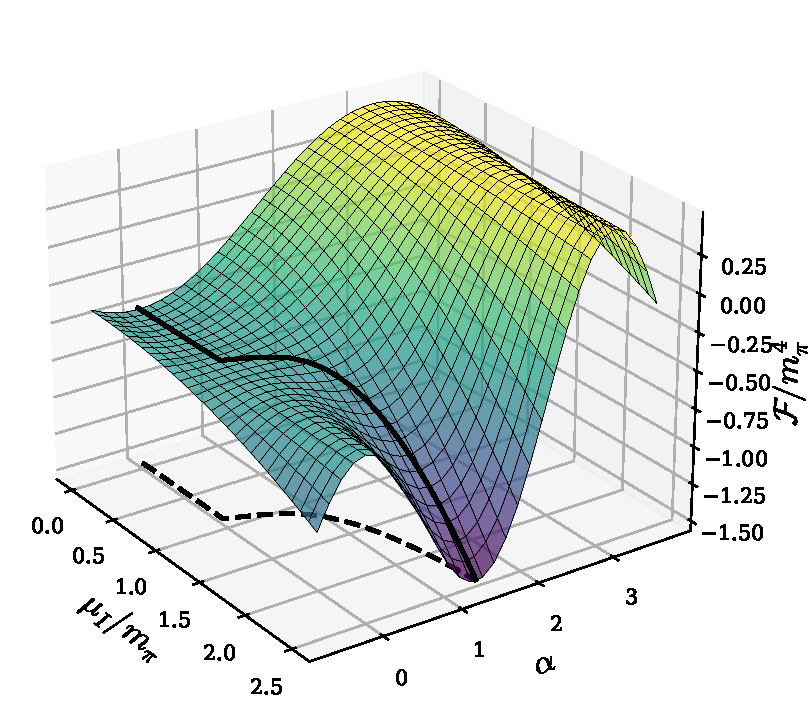
\includegraphics{figurer/numerics/free_energy_surface.pdf}
    \caption{The surface gives free energy as a function of $\mu_I$ and $\alpha$. $\alpha$ is the found by minimizing $\Ef$ for a given $\mu_I$. This leads to a curve across the free energy surface, as show in the plot.}
    \label{fig:free energy surface}
\end{figure}

\subsection*{One-loop contribution}
The one loop contribution to the free energy density is
\begin{equation}
    \label{one loop free energy}
    \Ef^{(1)}
    = - \frac{i}{V T} \frac{1}{2}
    \Tr{\ln\left( -\fdiff{S[\pi = 0]}{\pi_a(x), \pi_b(y)} \right)}.
\end{equation}
This can be evaluated using the rules for functional differentiation given in \autoref{section:Functional derivative}.
To leading order,
\begin{align}
    \fdiff{S[\pi = 0]}{\pi_a(x), \pi_b(y)}
    = \fdiff{}{\pi_a(x), \pi_b(y)}
    \int \dd^4 x \, \Ell^{(2)}_2
    = D_{ab}^{-1}(x - y).
\end{align}
Here, $\Ell^{(2)}_2$ is the quadratic part of the Lagrangian, as given in \cref{quadratic lagrangian}, and $D^{-1}$ is the corresponding inverse propagator of the pion fields,
\begin{equation}
    D_{ab}^{-1}(x-y) = 
    \left[
        - \delta_{ab}(\partial_x^2 + m^2_a)
        + m_{12}(\delta_{a1} \delta_{b2} - \delta_{a2}\delta_{b1}) \partial_{x, 0}
    \right] \delta(x-y)
\end{equation}
The inverse propagator is a matrix, which means that the determinant in \cref{one loop free energy} is both a matrix determinant, over the three pion indices, and a functional determinant.
In \autoref{section:propagator} we found the matrix part of the determinant in momentum space, which we can write using the dispersion relations of the pion fields
\begin{equation}
    \det(- D^{-1}) = \det(-p_0^2 + E_0^2) \det(-p_0^2 + E_+^2) \det(-p_0^2 + E_-^2).
\end{equation}
These dispersion relations are functions of the three-momentum $\vec p$, and are given in \cref{dispresion relation pi 0,dispresion relation pi pm}.
The functional determinant can therefore be evaluated as
\begin{align}
    \nonumber
    \Tr{\ln\left( -\fdiff{S[\pi = 0]}{\pi_a(x), \pi_b(y)} \right)}
    & = \ln \det(-p_0^2 + E_0^2) + \ln \det(-p_0^2 + E_+^2) + \ln \det(-p_0^2 + E_-^2) \\
    \nonumber
    & = \Tr{ \ln(-p_0^2 + E_0^2) + \ln(-p_0^2 + E_+^2)+  \ln(-p_0^2 + E_-^2) } \\
    & = (VT) \int \frac{\dd^4 p}{(2 \pi)^4} 
    \left[ \ln(-p_0^2 + E_0^2) + \ln(-p_0^2 + E_+^2) + \ln(-p_0^2 + E_-^2)  \right],
\end{align}
where we have used the identity $\ln\det M = \Tr \ln M $.
These terms all have the form
\begin{equation}
    \label{free energy logarithmic integral}
    I = \int \frac{\dd^4 p}{(2 \pi)^2} \ln(-p_0^2 + E^2),
\end{equation}
where $E$ is some function of the 3-momentum $\vec p$, but not $p_0$.
We use the trick
\begin{equation}
    \pdv{\alpha} \left(-p_0^2 + E^2\right)^{-\alpha} \Big|_{\alpha=0}
    = \pdv{\alpha} \exp\left[ -\alpha \ln\left(- p_0^2 + E^2\right)  \right] \Big|_{\alpha=0}
    = \ln\left(- p_0^2 + E^2\right),
\end{equation}
and then perform a Wick-rotation of the $p_0$-integral to write the integral on the form 
\begin{equation}
    I = i \pdv{\alpha} \int \frac{\dd^4 p}{(2 \pi)^4} \left(p_0^2 + E^2\right)^{-\alpha} \Big|_{\alpha=0},
\end{equation}
where $p$ now is a Euclidean four-vector.
The $p_0$ integral equals $\Phi_1(E, 1, \alpha)$, as defined in \autoref{def dimreg integral}. 
The result is therefore given by \autoref{result dimreg},
\begin{equation}
    \int \frac{\dd p_0}{2 \pi} (p_0^2 + E)^{-\alpha} 
    = \frac{E^{1-2\alpha}}{\sqrt{4 \pi}} \frac{\Gamma(\alpha-\frac{1}{2})}{\Gamma(\alpha)}.
\end{equation}
The derivative of the Gamma function is $\Gamma'(\alpha) = \psi(\alpha)\Gamma(\alpha)$, where $\psi(\alpha)$ is the digamma function.
Using
\begin{align}
    \diffp{}{\alpha} & \frac{\Gamma(\alpha - \frac{1}{2}) }{\Gamma(\alpha)} \Big|_{\alpha=0}
    = \Gamma\left(\alpha - \frac{1}{2}\right) \frac{\psi(\alpha - \frac{1}{2}) - \psi(\alpha)}{\Gamma(\alpha)} \Big|_{\alpha=0}
    = \sqrt{4 \pi}, \\
    & \frac{\Gamma(\alpha - \frac{1}{2}) }{\Gamma(\alpha)}\Big|_{\alpha=0} = 0,
\end{align}
we get
\begin{equation}
    I = i \int \frac{\dd^3 p}{(2 \pi)^3} E.
\end{equation}
We see that the result is what we would expect physically, the total energy is the integral of the energy of each mode.
This also agrees with the result from \autoref{appendix:thermal field theory} in low temperature limit $\beta \rightarrow \infty$.
This results in 
\begin{equation}
    \Ef^{(1)} = 
    \frac{1}{2} 
    \left[\int \frac{\dd^3 p}{(2\pi)^3} E_0 + \int  \frac{\dd^3 p}{(2\pi)^3} (E_+ + E_-)\right]
    = \Ef^{(1)}_{\pi_0} +\Ef^{(1)}_{\pi_\pm}.
\end{equation}
The first integral is identical to what we find for a free field in \autoref{section:free scalar field}, in the zero temperature limit $\beta \rightarrow \infty$.
These terms are all divergent, and must be regularized. 
We will use dimensional regularization, in which the integral is generalized to $d$ dimensions, and the $\overline{\mathrm{MS}}$-scheme, as described in \autoref{section: regualting free energy}.
Using the result for a free field \cref{free field regularized energy}, we get
\begin{equation}
    \label{Free energy pi 0}
    \Ef^{(1)}_{\pi_0} 
    = 
    - \mu^{-2 \epsilon}  \frac{1}{4} \frac{m_3^4}{(4\pi)^2} 
    \left( \frac{1}{\epsilon} + \frac{3}{2} + \ln \frac{\tilde \mu^2}{m_3^2} \right),
\end{equation}
where $\mu$ is the renormalization scale, a parameter with mass-dimension 1 which is introduced to ensure the action integral remains dimensionless during dimensional regularization.
$\tilde \mu$ is a related to $\mu$ as described in \cref{definition mu tilde MS bar}.

The contribution to the free energy from the $\pi_+$ and $\pi_-$ particles is more complicated, as the dispersion relation is given by
\begin{equation}
    E_\pm
    = 
    \sqrt{
        |\vv p|^2 +
        \frac{1}{2}
        \left(
            m_1^2 + m_2^2 + m_{12}^2 
        \right)
        \pm 
        \frac{1}{2}
        \sqrt{
            4|\vv p|^2m_{12}^2 
            +
            \left(
                m_1^2 + m_2^2 + m_{12}^2
            \right)^2
            - 4 m_1^2 m_2^2
        }
    }.
\end{equation}
This is not an integral we can easily do in dimensional regularization.
Instead, we will seek a function $f(|\vv p|)$ with the same UV-behavior, that is behavior for large $\vv p$, as $E_+ + E_-$.
If we then add $0 = f(|\vv p|) - f(|\vv p|)$ to the integrand, we can isolate the divergent behavior
\begin{equation}
    \Ef_{\pi_\pm}^{(1)}
    = 
    \frac{1}{2} \int \frac{\dd^3 p}{(2\pi)^3} [E_+ + E_- + f(|\vv p|) - f(|\vv p|)]
    = \Ef^{(1)}_{\mathrm{fin}, \pi_\pm } + \Ef^{(1)}_{\mathrm{div}, \pi_\pm}.
\end{equation}
This results in a finite integral, 
\begin{equation}
    \Ef^{(1)}_{\mathrm{fin}, \pi_\pm } = \frac{1}{2} \int \frac{\dd^3 p}{(2\pi)^3} [E_+ + E_- - f(|\vv p|)],
\end{equation}
which we can evaluate numerically, and isolate the divergence to
\begin{equation}
    \Ef^{(1)}_{\mathrm{div}, \pi_\pm }
    = 
    \frac{1}{2} \int \frac{\dd^3 p}{(2\pi)^3} f(|\vv p|),
\end{equation}
which we hopefully will be able to do in dimensional regularization.
We can explore the UV-behavior of $E_+ + E_-$ by expanding it in powers of $1 / \abs{\vv{p}}$,
\begin{align}
    \nonumber
    E_+ + E_-
    & = 
    2  \abs{\vv{p}}
    + \frac{m_{12} + 2(m_1^2 + m_2^2)}{4} \, {\abs{\vv{p}}}^{-1}
    - \frac{m_{12}^4 + 4 m_{12}^2(m_1^2 + m_2^2) + 8(m_1^4 + m_2^4)}{64}
    {\abs{\vv{p}}}^{-3}
    + \Oh[-5]{ \abs{\vv{p}}} 
    \\
    & = 
    a_1  \abs{\vv{p}}
    + a_2 \, {\abs{\vv{p}}}^{-1}
    + a_3
    {\abs{\vv{p}}}^{-3}
    + \Oh[-5]{ \abs{\vv{p}}}.
\end{align}
We have defined the new constants $a_i$ for brevity of notation.
As
\begin{equation}
    \int_{\R^3} \frac{\dd^3 p}{(2 \pi)^3} |\vv p|^{n}
    = C \int_{0}^\infty \dd p \, p^{2 + n}
\end{equation}
is UV divergent for $n \geq -3$, $f$ need to match the expansion of $E_+ + E_-$ up to and including $\Oh[-3]{|\vv{p}|}$ for $\Ef^{(1)}_{\mathrm{fin}, \pi_\pm }$ to be finite.
The most obvious choice for $f$ is
\begin{equation}
    f(|\vv p|) 
    = a_1  \abs{\vv{p}} + a_2 \, {\abs{\vv{p}}}^{-1} + a_3 \, {\abs{\vv{p}}}^{-3}.
\end{equation}
However, this introduces a new problem.
$f$ has the same UV-behavior as $E_+ + E_-$, but the last term diverges in the IR, that is for low $|\vv p|$.
This can be amended by introducing a mass term.
Let
\begin{equation}
    |\vv p|^{-3} 
    = 
    \left(\frac{1}{\sqrt{|\vv p|^2}}\right)^3 
    \longrightarrow 
    \left(\frac{1}{\sqrt{|\vv p|^2 + m^2}}\right)^3.
\end{equation}
For $|\vv p|^2 \rightarrow \infty$, this term is asymptotic to $|\vv p|^{-3}$, so it retains its UV behavior.
However, for $|\vv p| \rightarrow 0$, it now approaches $m^{-3}$, so the IR-divergence is gone.
The cost of this technique is that we have introduced an arbitrary mass parameter.
Any final result must thus be independent of the value of $m$ to be acceptable.

We will instead regularize the integral by defining $E_i = \sqrt{|\vv{p}|^2 + \tilde m_i^2}$, and $\tilde m_i^2 = m_i^2 + \frac{1}{4} m_{12}^2$.
Using the definition of the mass parameters, \cref{m1,m2,m3,m12}, we get
\begin{align}
    m_3^2 & = \bar m^2 \cos \alpha + \mu_ I^2 \sin^2 \alpha, \\
    \label{tilde m1}
    \tilde m_1^2 
    & 
    = m_1^2 + \mu^2 \cos\alpha^2
    = \bar m^2 \cos \alpha + \mu_I^2 \sin^2 \alpha
    = m_3^2 \\
    \label{tilde m2}
    \tilde m_2^2 
    & = m_2^2 + \mu^2 \cos\alpha^2
    = \bar m^2 \cos \alpha.
\end{align}
Finally, we define $f(|\vv p|) = E_1 + E_2$ which differ from $E_+ + E_-$ by $\Oh[-5]{|\vv p|}$, and is well-behaved in the IR.
This leads to a divergent integral the same form as in the case of a free scalar.
Thus, in the $\mathrm{\overline{MS}}$-scheme, 
\begin{equation}
    \Ef^{(1)}_{\mathrm{div}, \pi_\pm }
    =
    - \mu^{-2 \epsilon} \frac{1}{4} \frac{\tilde m_1^4}{(4\pi)^2} 
    \left(
        \frac{1}{\epsilon} + \frac{3}{2} + \ln \frac{\tilde \mu^2}{\tilde m_1^2}
    \right) 
    -  \mu^{-2 \epsilon} \frac{1}{4} \frac{\tilde m_2^4}{(4\pi)^2} 
    \left(
        \frac{1}{\epsilon} + \frac{3}{2} + \ln \frac{\tilde \mu^2}{\tilde m_2^2}
    \right) 
    + \mathcal{O}(\epsilon).
\end{equation}
We define
\begin{equation}
    \Ef^{(1)}_{\mathrm{fin}, \pi_\pm}
    = 
    \frac{1}{2} \int \frac{\dd^3 p}{(2\pi)^3} (E_+ + E_- - E_1 - E_2),
\end{equation}
which is a finite integral.
The total one-loop contribution is then, using \cref{tilde m1,tilde m2},
\begin{align}
    \Ef^{(2)}
    & = 
    \Ef^{(1)}_{\mathrm{fin}, \pi_\pm} 
    - \mu^{-2 \epsilon} \frac{1}{2}\frac{1}{(4\pi)^2}
    \left[
        \left( \frac{1}{\epsilon} + \frac{3}{2} + \ln \frac{\tilde \mu^2}{m_3^2 } \right)
        m_3^4
        +
        \frac{1}{2}
        \left( \frac{1}{\epsilon} + \frac{3}{2} + \ln \frac{\tilde \mu^2}{\tilde m_2^2} \right)
        \tilde m_2^4
    \right]
\end{align}

\subsection{Renormalization}
We have now regularized the divergences, so they can be handled in a well-defined way.
However, they are still there.
To get rid of them, we need to use renormalization.
The power counting scheme used when constructing the Effective Lagrangians ensures that all terms in $\Ell_{2n}$ is of order $p^{2n}$ in the pion momenta.\footnote{Remember that the pion mass $m_\pi = 2 f_\pi B$ is considered to be of order $p^2$.}
The tree level free energy from $\Ell_{2n}$ is thus of order $p^{2n}$.
The n-loop correction to the tree level result is then suppressed by $p^{2n}$~\cite{Gasser-Leutwyler:chiral,WeinbergPhenom}.
Our one-loop calculation using $\Ell_2$ therefore contains divergences of order $p^{4}$. 
Since $\Ell_4$ is, by construction, the most general possible Lagrangian at order $p^4$, it contains coupling constants which can be renormalized to absorb all these divergences.

The renormalized coupling constants in $\Ell_2$ have been calculated for $\mu_I = 0$~\cite{Gasser-Leutwyler:chiral}.
These are independent of $\mu_I$, and we can therefore use them in this calculation.
The renormalized coupling constants in the $\overline{\mathrm{MS}}$-scheme are related to the bare couplings through
\begin{align}
    l_i 
    & = 
    l_i^r \, \,
    - \frac{1}{2} \frac{\gamma_i }{(4 \pi)^2} 
    \left(\frac{1}{\epsilon} + 1 - \ln \mu^2\right),
    \quad \quad
    i \in \{1, ... 7\} 
    \\
    h_i 
    & = 
    h_i^r
    - \frac{1}{2} \frac{\delta_i }{(4 \pi)^2} 
    \left(\frac{1}{\epsilon} + 1 - \ln \mu^2 \right), 
    \quad \quad
    i \in \{1, ... 3\}.
\end{align}
(HVORDAN KAN VI HA log AV DIMENSJONSFULL STØRRELSE?).
Here, $\gamma_i$ and $\delta_i$ are numerical constants that are used to match the divergences.
The relevant terms are
\begin{gather}
    \gamma_1 = \frac{1}{3}, \quad
    \gamma_2 = \frac{2}{3}, \quad
    \gamma_3 = - \frac{1}{2}, \quad
    \gamma_4 = 2, \\
    \delta_1 = 2, \quad
    \delta_3 = 0.
\end{gather}
The bare coupling constants, though infinite, are independent of our renormalization scale $\mu$.
From this we obtain the renormalization group equations for the running coupling constants,
\begin{equation}
    \diff{\, l_i^r}{\ln \mu } = - \frac{\gamma_i}{(4 \pi)^2}, \quad
    \diff{\, h_i^r}{\ln \mu } = - \frac{\delta_i}{(4 \pi)^2}.
\end{equation}
These have the general solutions
\begin{equation}
    l_i^r 
    = \frac{1}{2} \frac{\gamma_i}{(2 \pi)^2} 
    \left( \bar l_i - \ln{\frac{\mu^2}{M^2}} \right),
    \quad
    h_i^r 
    = \frac{1}{2} \frac{\gamma_i}{(2 \pi)^2} 
    \left( \bar h_i - \ln{\frac{\mu^2}{M^2}} \right),
\end{equation}
where $\bar l_i$ and $\bar h_i$ are the values of the coupling constants (times a constant) measured at the energy $M$.
This only applies if the numerical constants $\gamma_i$/$\delta_i$ are non-zero.
If they are zero, then the renormalized constant is not running, and instead equal to its measured value at all energies.
The bare couplings are thus given by
\begin{equation}
    l_i = \frac{1}{2} \frac{\gamma_i}{(4 \pi)^2}
    \left(\bar l_i - 1 - \frac{1}{\epsilon} - \ln\frac{\mu^2}{M^2}\right), \quad
    h_i = \frac{1}{2} \frac{\delta_i}{(4 \pi)^2}
    \left(\bar h_i - 1 - \frac{1}{\epsilon} - \ln\frac{\mu^2}{M^2}\right)
\end{equation}
(HVOR BLE DET AV $\ln \mu$?)
The free energy at tree-level, at next-to-leading order is, according to \cref{NLO-L0}, 
\begin{align*}
    \Ef^{(0)}_4
    & 
    = - \Ell_4^{(0)} 
    \\
    & = 
    - (l_1 + l_2)\mu_I^4 \sin^4{\alpha}
    - (l_3 + l_4)(2 B_0 \bar m)^2 \cos^2{\alpha}
    - l_4 (2 B_0 \bar m ) \mu_I{}^2 \cos{\alpha} \sin^2{\alpha}
    \\
    & 
    \quad + l_4 (2B_0 \bar m )^2
    - h_1 (2B_0 \bar m)^2
    - h_3 (2B_0 \Delta m)^2
    % \\
    % & = 
    % - \frac{1}{2} \frac{1}{(4 \pi)^2}
    % \bigg[
    %     \frac{1}{3}
    %     \left( 
    %         \bar l_1 + 2 \bar l_2 - 3 - \frac{3}{\epsilon} - 3\ln \frac{\mu^2}{M^2}
    %     \right) \mu_I^4 \sin^4 \alpha
    %     +
    %     \frac{1}{2}
    %     \left(
    %         - \bar l_3 + 4 \bar l_4 - 3 - \frac{3}{\epsilon} - 3\ln \frac{\mu^2}{M^2}
    %     \right) (2 B_0 m)^4 \cos^2\alpha 
    %     \\
    %     &
    %     + 2 \left(\bar l_4 - 1 - \frac{1}{\epsilon} - \ln \frac{\mu^2}{M^2} \right)
    %     (2 B_0 m)^2 \mu_I^2 \cos\alpha \sin^2 \alpha
    %     + 2 (\bar l_4 - \bar h_1) (2B_0 \bar m )^2
    %     + \bar h_3 (2B_0 \Delta m)^2    
    % \bigg]
    \\
    & = 
    - \frac{1}{2} \frac{1}{(4 \pi)^2}
    \bigg[
        \frac{1}{3}
        \left( 
            \bar l_1 + 2 \bar l_2 - 3
        \right) \mu_I^4 \sin^4 \alpha
        +
        \frac{1}{2}
        \left(
            - \bar l_3 + 4 \bar l_4 - 3
        \right) (2 B_0 m)^4 \cos^2\alpha
        \\
        & \quad \quad \quad \quad \quad
        + 2 \left(\bar l_4 - 1\right)
        (2 B_0 m)^2 \mu_I^2 \cos\alpha \sin^2 \alpha
        \\
        & \quad \quad \quad \quad \quad
        - 
        \left(\frac{1}{\epsilon} + \ln \frac{\mu^2}{M^2}\right) 
        \left(
            \mu_I^4\sin^4\alpha + \frac{3}{2} (2 B_0 m)^4 \cos^2 \alpha
            + 2 (2 B_0 m)^2 \mu_I^2 \cos\alpha \sin^2 \alpha
        \right) 
        \\
        & \quad \quad \quad \quad \quad
        + 2 (\bar l_4 - \bar h_1) (2B_0 \bar m )^2
        + \bar h_3 (2B_0 \Delta m)^2
    \bigg] 
\end{align*}
Adding all the contribution to the free energy density, we get
\begin{align*}
    \Ef &=
    - f^2 \left((2 B_0 m)^2 \cos \alpha + \frac{1}{2}\mu_I^2 \sin^2 \alpha\right)
    + \Ef^{(1)}_{\mathrm{fin}, \pi_\pm}
    - \frac{1}{2}\frac{1}{(4 \pi)^2}
    \bigg[
        \frac{1}{3}
        \left( 
            \bar l_1 + 2 \bar l_2 + \frac{3}{2} + 3 \ln \frac{M^2}{m_3^2}
        \right) \mu_I^4 \sin^4 \alpha
        \\ 
        &
        +
        \frac{1}{2}
        \left(
            - \bar l_3 + 4 \bar l_4 + \frac{3}{2} + 2\ln \frac{M^2}{m_3^2}
            + \ln \frac{M^2}{\tilde m^2_2}
        \right) (2 B_0 m)^4 \cos^2\alpha 
        + 2 \left(\bar l_4 - \frac{1}{2} + \ln \frac{M^2}{m_3^2}\right)
        (2 B_0 m)^2 \mu_I^2 \cos\alpha \sin^2 \alpha
        \\
        & 
        + 2 (\bar l_4 - \bar h_1) (2B_0 \bar m )^2
        + \bar h_3 (2B_0 \Delta m)^2
    \bigg].
\end{align*}
\section{Thermodynamics}
(KIILDER)

The free energy\footnote{As we are in the grand canonical ensemble, this is the \emph{grand canonical} free energy, and not Helmholtz' free energy.}
is defined as
\begin{equation}
    \label{thermodynamic free energy}
    F = U - TS - \mu_I Q_I, \quad \dd F = - S \dd T - P \dd V - Q_I \dd \mu_I ,
\end{equation}
where $Q_I$ is the isospin charge, and $U$ is the energy.
As we have seen earlier, our system is homogenous.
This means that the free energy density is independent of volume, and thus $F = V \Ef$.
From  \cref{thermodynamic free energy} we see that the pressure is given by
\begin{equation}
    P = - \left(\diffp{F}{V}\right)_{T, \mu_I} = - \Ef.
\end{equation}
We are interested in the pressure relative to the state in which $\mu_I$ = 0. We therefore normalize $P(\mu_I=0) = 0$, which gives  
\begin{equation}
    P(\mu_I) = -(\Ef(\mu_I) - \Ef(\mu_I = 0))
\end{equation}
This is illustrated in \autoref{fig:pressure}.
\begin{figure}[h]
    \centering
    \vspace{-0.2cm}
    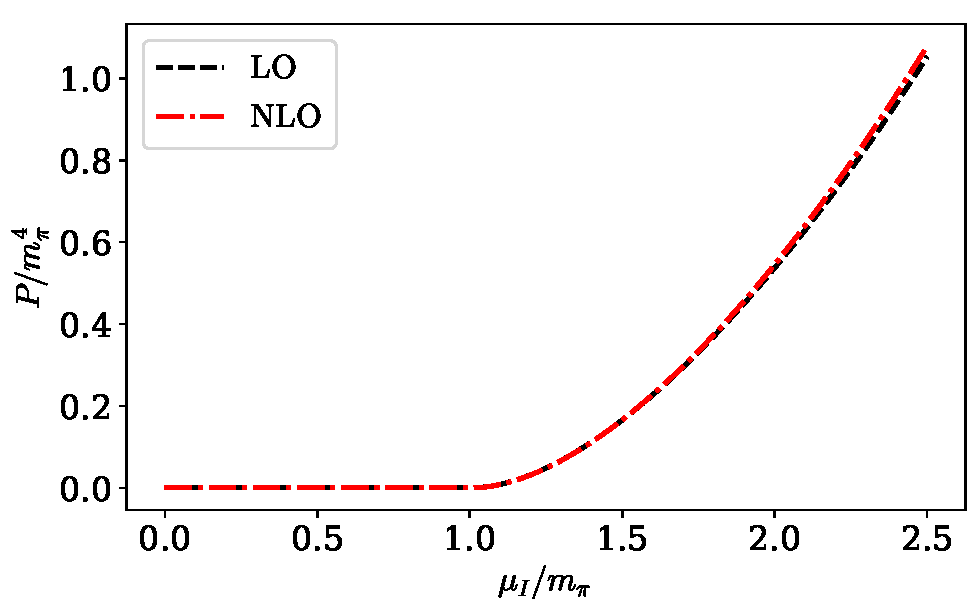
\includegraphics[width=0.7\textwidth]{figurer/numerics/pressure.pdf}
    \caption{The NLO and LO result for the pressure of the pions, as a function of $\mu_I$.}
    \label{fig:pressure}
\end{figure}

Likewise, the total isospin is proportional to volume, which means that the isospin density is
\begin{equation}
    n_I = \frac{Q_I}{V} = - \frac{1}{V} \left(\diffp{F}{\mu_I}\right)_{T, V}
    = - \diffp{\Ef}{\mu_I}.
\end{equation}
This gives 
\begin{align}
    \nonumber
    n_I & = 
    f^2 \mu_I \sin^2 \alpha
    - \diffp{\Ef_\mathrm{fin}}{\mu_I} \\
    & + \frac{1}{(4 \pi)^2}
    \left[
            \left(2\bar l_4+\ln\frac{M^2}{m_3^2}\right)\bar m^2 \mu_I \cos\alpha \sin^2 \alpha
            +\frac{1}{3}\left(2\bar l_1 + 4 \bar l_2 + 3\ln\frac{M^2}{m_3^2}\right)\mu_I^3 \sin^4 \alpha
    \right]
\end{align}
The isospin density, as a function of $\mu_I$, is shown in \autoref{fig:isospin_density}.
\begin{figure}[!h]
    \centering
    \vspace{-0.2cm}
    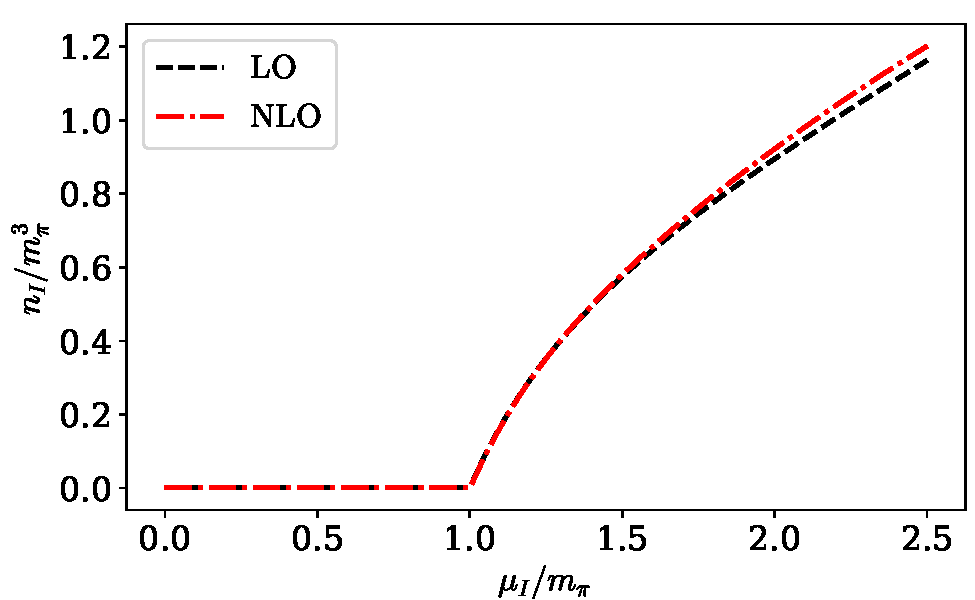
\includegraphics[width=0.7\textwidth]{figurer/numerics/isospin_density.pdf}
    \caption{The NLO and LO result for the isosopin densisty, as a function of $\mu_I$.}
    \label{fig:isospin_density}
\end{figure}

From \cref{thermodynamic free energy} we get the energy density, $u = U/V$, at $T = 0$ is given by
\begin{equation}
    u(\mu_I) = -P(\mu_I) + \mu_I n_I(\mu_I),
\end{equation}
where we again have normalized so that $u(\mu_I = 0) = 0$.
Now that we have both the dependence of pressure and energy density on the isospin chemical potential, we can trace out the line in the pressure-energy density plane, parametrized by $\mu_I$.
This is shown in \autoref{fig:equation of state}.
This is the equation of state of the system.

\begin{figure}[!h]
    \centering
    \vspace{-0.2cm}
    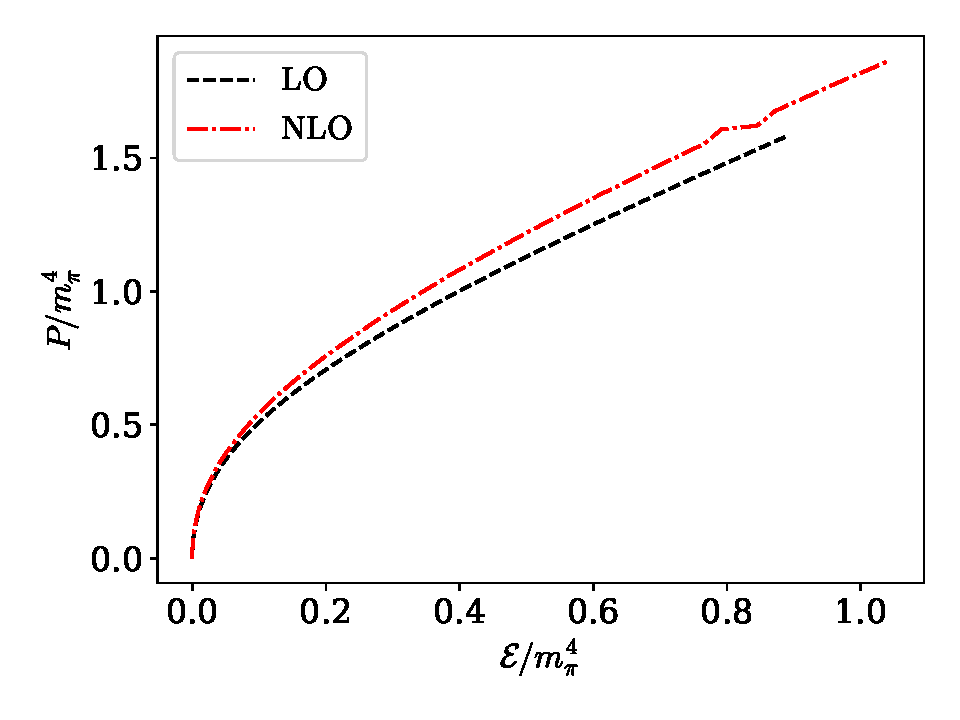
\includegraphics[width=0.7\textwidth]{figurer/numerics/energy_density.pdf}
    \caption{The equation of state of the system.}
    \label{fig:equation of state}
\end{figure}

\FloatBarrier

\subsection*{Phase transition}
(KILDER)

In our leading-order analysis, we saw that $\alpha$ was zero for $\mu_I \leq \bar m$, before it starts to increase for $\mu_I>\bar m$, and that $\bar = m_\pi$.
The behavior of $\alpha$ is illustrated in \autoref{fig:alpha}.
This is the hallmark of a phase transition, where $\alpha$ is the order parameter.
The behavior systems near points of phase transition is described by Landau theory.
Using \cref{leading order contribution free energy}, we can expand the leading-order free energy in $\alpha$,
\begin{align}
    \Ef
    & = -f^2 \bar m^2 + f^2 \frac{1}{2}(\bar m^2 - \mu_I^2)\alpha^2
    - \frac{1}{24} f^2 (\bar m^2 - 4 \mu_I^2) \alpha^4 + \Oh[5]{\alpha} \\
    & = \Ef(\alpha=0) + a(\mu_I)\alpha^2 + \frac{1}{2} b(\mu_I)\alpha^4 + \Oh[5]{\alpha},
\end{align}
to leading order.
Notice that near $\mu_I = \bar m$, $b > 0$.
As earlier, the equation that governs $\alpha'$ is
\begin{equation}
    \label{landau ginsburg lo}
    \diffp{\Ef}{\alpha} \bigg|_{\alpha=\alpha'} = 2 [a(\mu_I) + b(\mu_I) \alpha^2] \alpha = 0.
\end{equation}
If $a>0$, then $\alpha' = 0$ will be the only solution, which gives us the criterion for a phase transition 
\begin{equation}
    a(\mu_I) = 0,
\end{equation}
which again gives $\mu_I = \bar m$.
Near $\mu_I = \bar m$, we can write
\begin{equation}
    a = - a_0 (\mu_I - \bar m), \quad b = b_0,
\end{equation}
where $a_0$ and $b_0$ are positive constants, so the solution to \cref{landau ginsburg lo} for $\mu_I>\bar m$
\begin{equation}
    \alpha(\mu_I) = \sqrt{\frac{a_0}{b_0}} (\mu_I - \bar m)^{1/2}.
\end{equation}
The order parameter $\alpha$ changes continuously as the system undergoes phase-transition.
This means we have a \emph{second order} phase transition.
However, if $b < 1$ near $\mu_I = \bar m$, this is not a valid solution, so we must expand $\Ef$ further to show if the phase transition is continuous or not.
The difference is illustrated in \autoref{fig:phase transition}.
\begin{figure}
    \centering
    \begin{subfigure}{0.49\textwidth}
        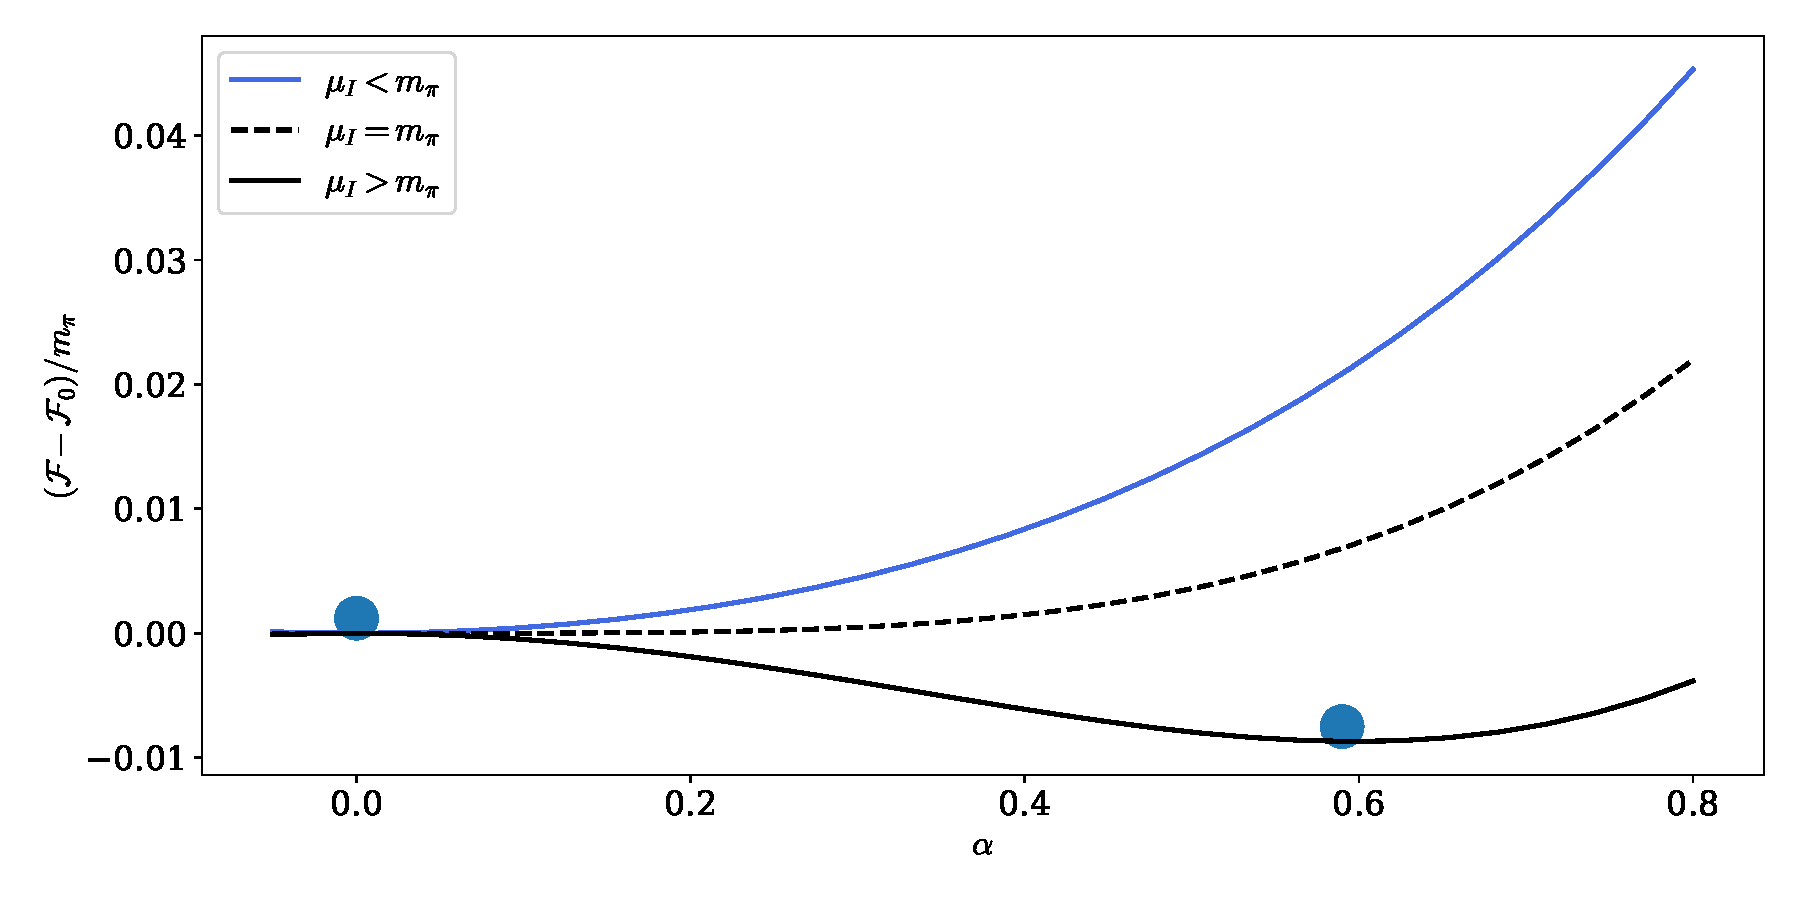
\includegraphics[width=\textwidth]{figurer/numerics/phase_transition.pdf}
    \end{subfigure}
    \begin{subfigure}{0.49\textwidth}
        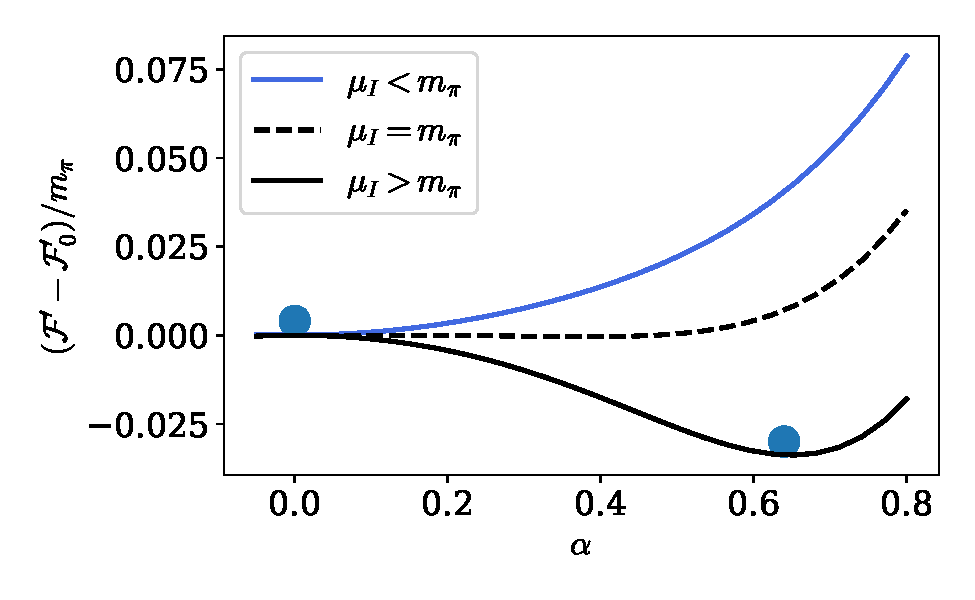
\includegraphics[width=\textwidth]{figurer/numerics/phase_transition2.pdf}
    \end{subfigure}
    \caption{The plot on the left shows normalized free energy density as a function of $\alpha$, in the two different phases. The plot on the right shows the same, but with a free energy $\Ef'$ that have been modified so that $b(\mu_I=\bar m)<0$.
    In the first case, the minima transitions continuous, while in the second it jumps.}
    \label{fig:phase transition}
\end{figure}

% Due to symmetry of the system under $\alpha \rightarrow -\alpha$, the expansion of $\Ef$ should only contain even powers.
% This can be certified to leading order by explicit calculation.
% We therefore write,
% \begin{equation}
%     \Ef = \Ef(\alpha = 0) + a \alpha^2 - \frac{1}{2} b \alpha^4 + \frac{1}{3} c \alpha^6
%     + \Oh[8]{\alpha}.
% \end{equation}
% We assume that near $\bar m = \mu_I$, we can write $a = -a_0(\mu_I - \bar m), \, b = -b0 ,½$ and $c = c_0$, where all the constants are positive.
% The equation for $\alpha'$ is now
% \begin{equation}
%     2\alpha [a - \alpha^3 (b - c \alpha^3 )] = 0
% \end{equation}
% We still have the $\alpha' = 0$ for $\mu_I < \bar m$.
% For $\mu_I> \bar m$, we get the solutions
% \begin{equation}
%     \alpha^3 = \frac{1}{2} \left( \frac{b}{c} \pm \sqrt{\left(\frac{b}{c} \right)^2- 4 \frac{a}{c}} \right)
%     = \frac{b_0}{2c_0} \left(1 \pm \sqrt{1- 4 (\mu_I - \bar m) \frac{a_0c_0}{b_0^2}} \right).
% \end{equation}
% Taking the second derivative, 
% \begin{equation}
%     \Ef' = a - (3 b - 5c \alpha^2)\alpha^2,
% \end{equation}



In the vacuum phase, $\alpha' = 0$, the ground state is given by 
\begin{equation}
    \Sigma(\pi = 0) = \Sigma_0 = \one,
\end{equation}
where we have use \cref{sigma}.
Under $H = SU(2)_V$, $\Sigma$ transforms as
\begin{equation}
    \Sigma(x) \rightarrow \Sigma'(x) = V \Sigma(x) V^\dagger,
    \quad
    V = \exp{i \theta_a \tau_a},
\end{equation}
which means that the vacuum phase ground state is invariant under $H$.
However, for $\alpha = 0$, the ground state is shifted to
\begin{equation}
    \Sigma(\pi=0) = A_\alpha \Sigma_0 A_\alpha = \exp{i \alpha \tau_1}.
\end{equation}
The generators $\tau_2$ and $\tau_3$ are broken.
The new ground state corresponds to a condensate of the $\pi_1$-particle, as it is defined in the vacuum state.
In \autoref{fig:masses}, we saw that the mass of the $m_-$ particle vanishes, so we identify this particle with the corresponding Goldstone mode.
There is only one Goldstone mode, however this is not a Lorentz invariant system, in which case we cannot guarantee one massless mode per broken generator. (ER DETTE RIKTIG?)

To find the value of $\mu_I$ to next-to-leading order, we must expand the NLO free energy in powers of $\alpha$
When we expand the static, second order Lagrangian to $\alpha^2$, we get
\begin{align}
    \Ef_4^{(0)}
    &= - (l_3 + l_4)\bar m^4 + [(l_3 + l_4)\bar m^4 -l_4 \bar m^2\mu_I^2]\alpha^2
    % \\
    % &
    % = \mu^{-2\epsilon} \frac{1}{(4\pi)^2}
    % \left[
    %     \left(
    %         -\frac{1}{4}(\bar l_3 - 1 - \frac{1}{\epsilon} - \ln\frac{\tilde \mu^2}{M^2})
    %         + (\bar l_4 - 1 - \frac{1}{\epsilon} - \ln\frac{\tilde \mu^2}{M^2})
    %     \right)\bar m^4
    %     -(\bar l_4 - 1 - \frac{1}{\epsilon} - \ln\frac{\tilde \mu^2}{M^2}) \bar m^2\mu_I^2
    % \right]\alpha^2
    % + \Oh[3]{\alpha}
    % \\
    % &
    % = \const + \mu^{-2\epsilon} \frac{1}{(4\pi)^2}
    % \left[
    %     \frac{3}{4}
    %     \left(
    %         \frac{4}{3}\bar l_4 - \frac{1}{3}\bar l_3 - 1 - \frac{1}{\epsilon} - \ln\frac{\tilde \mu^2}{M^2}
    %     \right)\bar m^4
    %     -
    %     \left(
    %         \bar l_4 - 1 - \frac{1}{\epsilon} - \ln\frac{\tilde \mu^2}{M^2}
    %     \right) 
    %     \bar m^2\mu_I^2
    % \right]\alpha^2
    % + \Oh[3]{\alpha}
    \\
    & =
    \const + 
    \frac{\mu^{-2\epsilon}}{(4\pi)^2}
    \left[
        \left(
            \bar l_4 - \frac{1}{4}\bar l_3
        \right)\bar m^4
        -\bar l_4\bar m^2\mu_I^2
        -\left(
            1 + \frac{1}{\epsilon} + \ln\frac{\tilde \mu^2}{M^2}
        \right)
        \left(\frac{3}{4}\bar m^2 - \mu_I^2\right)\bar m^2
    \right]\alpha^2,
\end{align}
where $\const$ is independent of $\alpha$, and thus not of interest.
From the one-loop correction, we have the contributions
\begin{equation}
    \Ef_2^{(1)} = i \frac{1}{2}\int \frac{\dd^4 p}{(2\pi)^2} \ln(-p^2 + m_3^2)
    +  i \frac{1}{2} \int \frac{\dd^4 p}{(2\pi)^2} \ln[(-p^2 + m_1^2)(-p^2 + m_2^2) - p_0^2 m_{12}^2]
\end{equation}
% We have already evaluated the first integral when ca
The first integral is the same free energy contribution from the $\pi_0$-particle as we have calculated earlier, and it reads
\begin{equation}
    \Ef_{\pi_0} 
    = i \frac{1}{2}\int \frac{\dd^4 p}{(2\pi)^2} \ln(-p^2 + m_3^2)
    = - \mu^{-2\epsilon}\frac{1}{4} \frac{m_3^4}{(4 \pi)^2}
    \left(\frac{1}{\epsilon} + \frac{3}{2} + \ln \frac{\tilde \mu^2}{m_3^2}\right).
\end{equation}
The mass $m_3$ is dependent on $\alpha$, and has the expansion
\begin{align*}
    % m_3^2 
    % &= \bar m^2 + \frac{1}{2}(2\mu_I^2 - \bar m^2)\alpha^2+ \Oh[3]{\alpha}, \\
    m_3^4
    &= \bar m^4 + \bar m^2(2\mu_I^2 - \bar m^2)\alpha^2+ \Oh[3]{\alpha}, \\
    \ln \frac{\mu^2}{m_3^2}
    &=
    \ln \frac{\mu^2}{\bar m_3^2} - \frac{1}{2} \frac{(2\mu_I^2 - \bar m^2)}{\bar m^2}+ \Oh[3]{\alpha}.
\end{align*}
In the second integral, we rewrite the argument of the logarithm as
\begin{equation}
    (-p^2 + m_1^2)(-p^2 + m_2^2) - p_0^2 m_{12}^2
    =  \left[-p^2 + \frac{1}{2}(m_1^2 + m_2^2)\right]^2 - p_0^2 m_{12}^2 - \frac{1}{4}(m_1^2 - m_2^2)^2.
\end{equation}
When we calculate the $\alpha$ dependence of the last term, we get  $(m_1^2 - m_2^2)^2 = \mu^4 \sin^4\alpha = \Oh[4]{\alpha}$, which means that for our purposes, we can ignore this term.
We further rewrite the remaining expression by factoring it,
\begin{equation}
    \left[-p^2 + \frac{1}{2}(m_1^2 + m_2^2)\right]^2 - p_0^2 m_{12}^2
    = \left[-p^2 + \frac{1}{2}(m_1^2 + m_2^2) - p_0 m_{12} \right]
    \left[-p^2 + \frac{1}{2}(m_1^2 + m_2^2) + p_0 m_{12} \right]
\end{equation}
% Each of these can be brought into a form so that we can perform the integral after a change of variables, through
% With a change of 
We then complete the square in each of the factors,
\begin{equation}
    - p^2 + \frac{1}{2}(m_1^2 + m_2^2) \pm p_0 m_{12}
    = - \left(p_0 \mp \frac{1}{2}m_{12}\right)^2 + |\vv p|^2 + m_4^2,
\end{equation}
where
\begin{align}
    m_4^2 &= \frac{1}{2}\left(m_1^2 +m_2^2 +\frac{1}{2}m_{12}\right)
    % = \bar m^2 \cos\alpha - \frac{1}{2} \mu_I^2 (\cos 2\alpha + \cos^2 \alpha - 2\cos^2\alpha)
    = \bar m^2 \cos\alpha + \frac{1}{2} \mu_I^2 \sin^2 \alpha, \\
    % M^2
    % &= \bar m^2 -\frac{1}{2}(m^2 + \mu_I^2) \alpha^2 + \Oh[3]{\alpha}, \\
    m_4^4
    &= \bar m^4 - \bar m^2(m^2 + \mu_I^2) \alpha^2 + \Oh[3]{\alpha}, \\
    \ln \frac{\mu^2}{m_4^2} 
    &= \ln \frac{\mu_I^2}{\bar m^2} + \frac{1}{2}\frac{\bar m^2 + \mu_I^2}{\bar m^2}\alpha^2
    + \Oh[3]{\alpha}.
\end{align}
After a shift of variables, the integral has the same form as the logarithmic integrals we have calculated earlier, which gives us the result
\begin{equation}
    \Ef_{\pi_\pm}
    = i \int \frac{\dd^4}{(2\pi)^4}
    \ln(-p^2 + M^2)
    = 
    - \mu^{-2\epsilon}\frac{1}{2} \frac{M^4}{(4 \pi)^2}
    \left(\frac{1}{\epsilon} + \frac{3}{2} + \ln \frac{\tilde \mu^2}{M^2}\right)
\end{equation}
Combining these two contributions to the one-loop correction of the free energy gives
\begin{align*}
    \Ef_2^{(1)}
    &=
    \mathrm{const.}
    +
    \frac{\mu^{-2 \epsilon } }{(4 \pi)^2} 
    \left(1 + \frac{1}{\epsilon} + \ln \frac{\tilde \mu^2}{m^2}\right)
    \left(\frac{3}{4}m^2 - \mu_I^2\right)
    \bar m^2 \alpha^2
\end{align*}
We see that again, the $\epsilon^{-1}$ will cancel when we combine the NLO-terms, and we get
\begin{align}
    \tilde \Ef_1
    & = 
    \const+ 
    \frac{1}{(4\pi)^2}
    \left[
        \left(
            \bar l_4 - \frac{1}{4}\bar l_3
        \right)\bar m^4
        -\bar l_4\bar m^2\mu_I^2
        + \ln\frac{M^2}{\bar m^2}
        \left(\frac{3}{4}\bar m^2 - \mu_I^2\right)\bar m^2
    \right]\alpha^2
    + \Oh[3]{\alpha}.
\end{align}
The total NLO free energy, up to second order in $\alpha$, is
(HVOR BLE DET AV LOG? TROR DET ER 1 + HØYERE ORDEN. SJEKK!)
\begin{equation}
    \Ef_{\mathrm{NLO}}
    =
    \Ef_{\mathrm{NLO}}(\alpha = 0)
    +
    \frac{1}{2} f^2 \bar m^2
    \left(
        1
        -
        \frac{1}{2}
        \frac{\bar l_3 - 4 \bar l_4}{(4 \pi)^2} \frac{\bar m^2}{f^2}
    \right)\alpha^2
    - \frac{1}{2}f^2 \mu_I^2
    \left(
        1
        +
        \frac{2 \bar l_4}{(4 \pi)^2}
        \frac{\bar m^2}{f^2}
    \right) \alpha^2
    + \Oh[3]{\alpha}.
\end{equation}
We now insert the physical constants $f_\pi$ and $m_\pi$, by using the next-to-leading order expressions \cref{equation bare mass} and \cref{equation bare decay constant}.
First, notice that
\begin{equation}
    f_\pi^2 m_\pi^2
    = f^2 \bar m^2
    \left(
        1 - \frac{1}{2} \frac{\bar l_3 - 4 \bar l_4}{(4 \pi)^2} \frac{\bar m^2}{f^2}
        +
        \Oh[]{\frac{\bar m^4}{f^4}}
    \right)
\end{equation}
This means that, to leading order,
\begin{equation}
    \Ef_{\mathrm{NLO}}
    =
    \Ef_{\mathrm{NLO}}(\alpha = 0)
    + \frac{1}{2}f_\pi^2 (m_\pi^2 - \mu_I^2 )\alpha^2
    + \Oh[3]{\alpha}.
\end{equation}
This shows that the phase transition happens at $\mu_I = m_\pi$, also at next-to-leading order.

\section{Phase transition}

Our leading-order analysis showed us that $\alpha$ is zero for $\mu_I \leq \bar m$, and then increases continuously for $\mu_I>\bar m$.
Furthermore, $\bar m = m_\pi$ to leading-order.
Thi behavior is illustrated in \autoref{fig:alpha}.
This is the hallmark of a phase transition, where $\alpha$ is the order parameter.
The behavior of systems near points of phase transition is described by Landau theory~\cite{Peskin:IntroQFT}.
Using \cref{leading order contribution free energy}, we can expand the leading-order free energy in $\alpha$,
\begin{align}
    \nonumber
    \Ef
    & = -f^2 \bar m^2 + f^2 \frac{1}{2}(\bar m^2 - \mu_I^2)\alpha^2
    - \frac{1}{24} f^2 (\bar m^2 - 4 \mu_I^2) \alpha^4 + \Oh[5]{\alpha} \\
    & = \Ef(\alpha=0) + a(\mu_I)\alpha^2 + \frac{1}{2} b(\mu_I)\alpha^4 + \Oh[5]{\alpha}.
\end{align}
Notice that near $\mu_I = \bar m$, $b > 0$.
As earlier, the equation that governs $\alpha$ is
\begin{equation}
    \label{landau ginsburg lo}
    \diffp{\Ef}{\alpha} = 2 [a(\mu_I) + b(\mu_I) \alpha^2] \alpha = 0.
\end{equation}
If $a>0$, then $\alpha = 0$ will be the only solution, which gives us the criterion for a phase transition 
\begin{equation}
    a(\mu_I) = 0.
\end{equation}
As expected, this criterion is fulfilled at $\mu_I = \bar m$.
Near $\mu_I = \bar m$, we can write
\begin{equation}
    a = - a_0 (\mu_I - \bar m), \quad b = b_0,
\end{equation}
where $a_0$ and $b_0$ are positive constants, so the solution to \cref{landau ginsburg lo} for $\mu_I>\bar m$ is
\begin{equation}
    \alpha(\mu_I) = \sqrt{\frac{a_0}{b_0}} (\mu_I - \bar m)^{1/2}.
\end{equation}
The free energy around the phase transition is illustrated in \autoref{fig:phase transition}.
\begin{figure}[h]
    \centering
    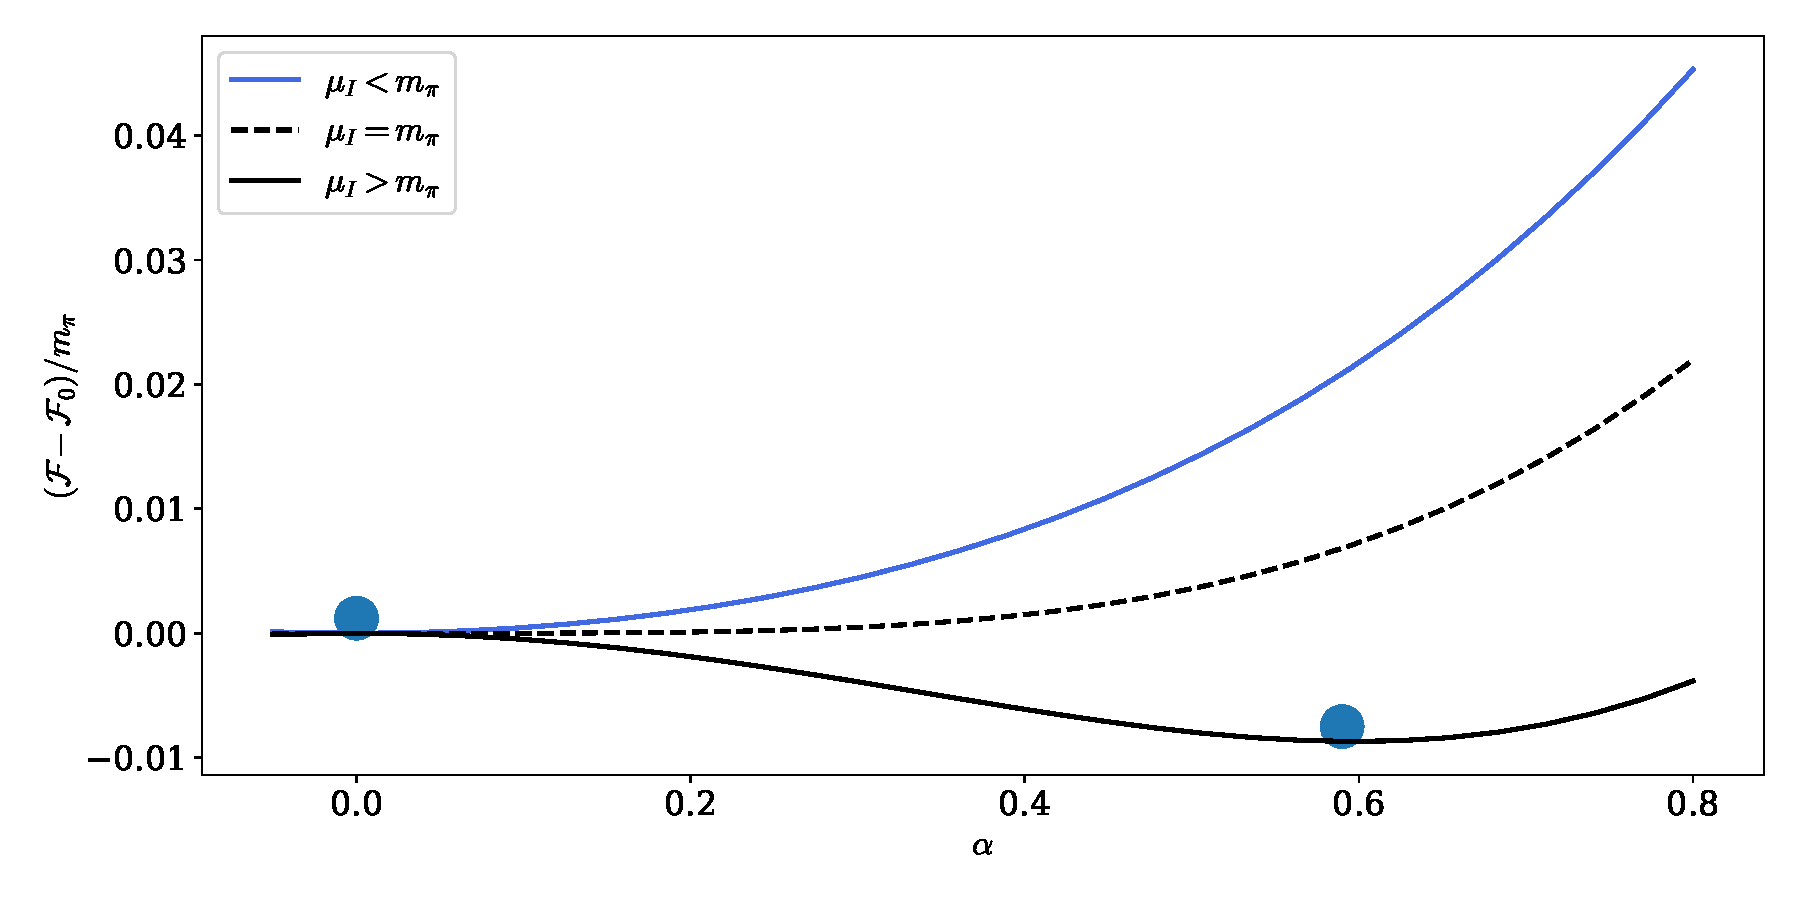
\includegraphics[width=0.9\textwidth]{figurer/numerics/phase_transition.pdf}
    \caption{The plot shows normalized free energy density as a function of $\alpha$, in the two different phases. Each line is a constant $\mu_I$ slice of the surface in \autoref{fig:free energy surface}.}
    \label{fig:phase transition}
\end{figure}

The order parameter $\alpha$ changes continuously as the system transitions phase.
This means we have a \emph{second order} phase transition.
The power-law behavior, $\alpha \propto (\mu_I - \mu_I^c)^\beta$, is typical of systems near a phase transition.
The exponent $\beta$, which in this case equals $1/2$, is called a \emph{critical exponent}.
If we have a system where $b < 0$ near $\mu_I = \bar m$, then we must expand $\Ef$ further to show if the phase transition is continuous or not.
\autoref{fig:free energy surface 2} shows the free energy surface but modified so that $b_0 < 0$, together with the corresponding value of $\alpha$, which now changes discontinuously at the point of phase transition.
\begin{figure}[h]
    \centering
    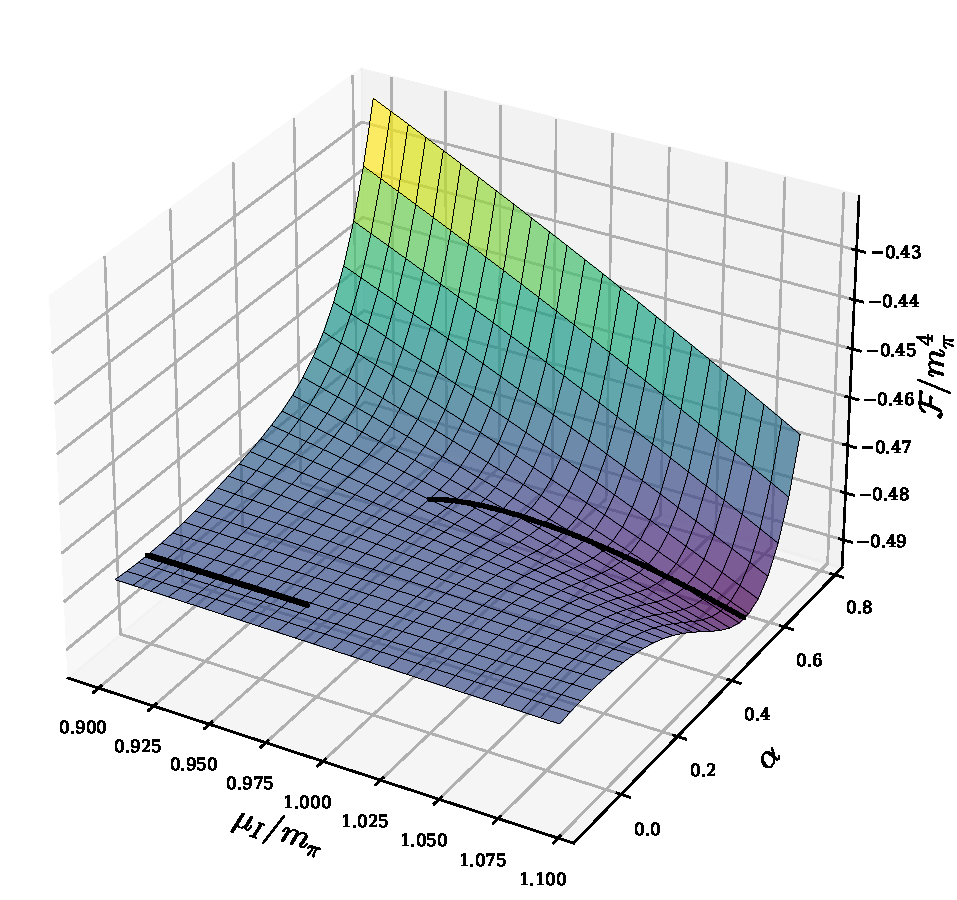
\includegraphics[width=0.7\textwidth]{figurer/numerics/free_energy_surface2.pdf}
    \caption{The surface is free energy density, only modified so that $b_0<0$. The black line traces out the minimum for each value of $\mu_I$, which jumps discontinuously at the point of phase transition.}
    \label{fig:free energy surface 2}
\end{figure}


In the vacuum phase, $\alpha = 0$, the ground state is given by 
\begin{equation}
    \Sigma(\pi = 0) = \Sigma_0 = \one,
\end{equation}
where we have used \cref{sigma}.
Under $H = SU(2)_V$, $\Sigma$ transforms as
\begin{equation}
    \Sigma(x) \rightarrow \Sigma'(x) = V \Sigma(x) V^\dagger,
    \quad
    V = \exp{i \frac{1}{2} \theta_a \tau_a},
\end{equation}
We see that the vacuum phase ground state is invariant under $H$.
However, for $\alpha \neq 0$, the ground state is shifted to
\begin{equation}
    \Sigma(\pi=0) = A_\alpha \Sigma_0 A_\alpha = \exp{i \alpha \tau_1}.
\end{equation}
This is not, in general, invariant under transformations in $H$. 
The generators $\tau_2$ and $\tau_3$ are broken.
In \autoref{fig:masses}, we saw that the mass of the $m_-$ particle vanishes, so we identify this particle with the corresponding Goldstone mode.
There is only one Goldstone mode. 
However, this is not a Lorentz invariant system, in which case we cannot guarantee one massless mode per broken generator.
In \autoref{section:leading order lagrangian}, we defined
\begin{equation}
    \alpha = \frac{1}{f} \sqrt{\pi_a^0 \pi_a^0},
\end{equation}
where $\pi_a^0$ was the ground state expectationvalue of the pion fields, as defined in the vacuum phase, when $\mu_I \neq 0$.
The new ground state thus corresponds to a condensate of pions.
The isospin symmetry $\SU(3)_V$ is not a perfect symmetry of the QCD Lagrangian, but is explicitly broken by the mass term
\begin{equation}
    \bar q m q = \frac{1}{2} \bar q [(m_u + m_d) \one + (m_u - m_d)\tau_3] q.
\end{equation}
This term, however, is invariant under the subgroup $\U(1)_{I_3} \subset \SU(2)_V$, generated by $\tau_3$.
If we write out a generic element from this subgroup,
\begin{equation}
    U = e^{i \theta \tau_3} = 
    \begin{pmatrix}
        e^{i\theta} & 0 \\
        0 & e^{-i \theta}
    \end{pmatrix},
\end{equation}
we se that this corresponds to rotating the phase of the up and down quark, but not rotating them into eachother.
Thus, the pion condensate spontaneously breaks an exact symmetry of the two-flavor QCD Lagrangian, and we expect the corresponding Goldstone mode to remain massless outside the chiral limit.

To find the value of $\mu_I$ to next-to-leading order, we must expand the NLO free energy in powers of $\alpha$
When we expand the static, second order Lagrangian to $\alpha^2$, we get
\begin{align}
    \nonumber
    \Ef_4^{(0)}
    &= - (l_3 + l_4)\bar m^4 + [(l_3 + l_4)\bar m^4 -l_4 \bar m^2\mu_I^2]\alpha^2
    \\
    & =
    \const + 
    \frac{\mu^{-2\epsilon}}{(4\pi)^2}
    \left[
        \left(
            \bar l_4 - \frac{1}{4}\bar l_3
        \right)\bar m^4
        -\bar l_4\bar m^2\mu_I^2
        -\left(
            1 + \frac{1}{\epsilon} + \ln\frac{\tilde \mu^2}{M^2}
        \right)
        \left(\frac{3}{4}\bar m^2 - \mu_I^2\right)\bar m^2
    \right]\alpha^2 + \mathcal{O}(\epsilon),
\end{align}
where $\const$ is independent of $\alpha$, and thus not of interest.
From the one-loop correction, we have the contributions
\begin{equation}
    \Ef_2^{(1)} = i \frac{1}{2}\int \frac{\dd^4 p}{(2\pi)^2} \ln(-p^2 + m_3^2)
    +  i \frac{1}{2} \int \frac{\dd^4 p}{(2\pi)^2} \ln[(-p^2 + m_1^2)(-p^2 + m_2^2) - p_0^2 m_{12}^2].
\end{equation}
The first integral is the same free energy contribution from the $\pi_0$-particle as we have calculated earlier in \cref{Free energy pi 0}, and it reads
\begin{equation}
    \Ef_{\pi_0}^{(1)}
    = i \frac{1}{2}\int \frac{\dd^4 p}{(2\pi)^2} \ln(-p^2 + m_3^2)
    = - \mu^{-2\epsilon}\frac{1}{4} \frac{m_3^4}{(4 \pi)^2}
    \left(\frac{1}{\epsilon} + \frac{3}{2} + \ln \frac{\tilde \mu^2}{m_3^2}\right) + \mathcal{O}(\epsilon).
\end{equation}
The mass $m_3$ is dependent on $\alpha$, and has the expansion
\begin{align*}
    m_3^4
    &= \bar m^4 + \bar m^2(2\mu_I^2 - \bar m^2)\alpha^2+ \Oh[4]{\alpha}, \\
    \ln \frac{\mu^2}{m_3^2}
    &=
    \ln \frac{\mu^2}{\bar m_3^2} - \frac{1}{2} \frac{(2\mu_I^2 - \bar m^2)}{\bar m^2}+ \Oh[4]{\alpha}.
\end{align*}
In the second integral, we rewrite the argument of the logarithm as
\begin{equation}
    (-p^2 + m_1^2)(-p^2 + m_2^2) - p_0^2 m_{12}^2
    =  \left[-p^2 + \frac{1}{2}(m_1^2 + m_2^2)\right]^2 - p_0^2 m_{12}^2 - \frac{1}{4}(m_1^2 - m_2^2)^2.
\end{equation}
When we calculate the $\alpha$ dependence of the last term, we get  $(m_1^2 - m_2^2)^2 = \mu^4 \sin^4\alpha = \Oh[4]{\alpha}$, which means that for our purposes, we can ignore this term.
We further rewrite the remaining expression by factoring it,
\begin{equation}
    \left[-p^2 + \frac{1}{2}(m_1^2 + m_2^2)\right]^2 - p_0^2 m_{12}^2
    = \left[-p^2 + \frac{1}{2}(m_1^2 + m_2^2) - p_0 m_{12} \right]
    \left[-p^2 + \frac{1}{2}(m_1^2 + m_2^2) + p_0 m_{12} \right].
\end{equation}
We then complete the square in each of the factors,
\begin{equation}
    - p^2 + \frac{1}{2}(m_1^2 + m_2^2) \pm p_0 m_{12}
    = - \left(p_0 \mp \frac{1}{2}m_{12}\right)^2 + |\vv p|^2 + m_4^2,
\end{equation}
where
\begin{align}
    m_4^2 &= \frac{1}{2}\left(m_1^2 +m_2^2 +\frac{1}{2}m_{12}\right)
    = \bar m^2 \cos\alpha + \frac{1}{2} \mu_I^2 \sin^2 \alpha, \\
    m_4^4
    &= \bar m^4 - \bar m^2(m^2 + \mu_I^2) \alpha^2 + \Oh[4]{\alpha}, \\
    \ln \frac{\mu^2}{m_4^2} 
    &= \ln \frac{\mu_I^2}{\bar m^2} + \frac{1}{2}\frac{\bar m^2 + \mu_I^2}{\bar m^2}\alpha^2
    + \Oh[4]{\alpha}.
\end{align}
After a shift of variables, the integral has the same form as the logarithmic integrals we have calculated earlier, which gives us the result
\begin{equation}
    \Ef_{\pi_\pm}
    = i \int \frac{\dd^4}{(2\pi)^4}
    \ln(-p^2 + m_4^2)
    = 
    - \mu^{-2\epsilon}\frac{1}{2} \frac{m_4^4}{(4 \pi)^2}
    \left(\frac{1}{\epsilon} + \frac{3}{2} + \ln \frac{\tilde \mu^2}{m_4^2}\right)+ \mathcal{O}(\epsilon).
\end{equation}
Combining these two contributions to the one-loop correction of the free energy gives
\begin{align*}
    \Ef_2^{(1)}
    &=
    \mathrm{const.}
    +
    \frac{\mu^{-2 \epsilon } }{(4 \pi)^2} 
    \left(1 + \frac{1}{\epsilon} + \ln \frac{\tilde \mu^2}{m^2}\right)
    \left(\frac{3}{4}m^2 - \mu_I^2\right)
    \bar m^2 \alpha^2+ \mathcal{O}(\epsilon).
\end{align*}
We see that again, the $\epsilon^{-1}$ will cancel when we combine the NLO-terms.
Setting $\epsilon = 0$, the NLO correction to the free energy becomes
\begin{align}
    \tilde \Ef_1
    & = 
    \const+ 
    \frac{1}{(4\pi)^2}
    \left[
        \left(
            \bar l_4 - \frac{1}{4}\bar l_3
        \right)\bar m^4
        -\bar l_4\bar m^2\mu_I^2
        + \ln\frac{M^2}{\bar m^2}
        \left(\frac{3}{4}\bar m^2 - \mu_I^2\right)\bar m^2
    \right]\alpha^2
    + \Oh[4]{\alpha}.
\end{align}
All coupling constants are measured at $M = m_\pi$.
Using this in the logarithm gives,
\begin{equation}
    \ln \frac{M^2}{\bar m^2}
    = \ln \frac{m_\pi^2}{\bar m^2}
    = \ln \left[1 + \Oh[2]{(\bar m/f)} \right]
    = \Oh[2]{(\bar m/f)}.
\end{equation}
The term proportional to the logarithm thus vanishes to next-to-leading order.
Combining these expressions give total NLO free energy, up to second order in $\alpha$, is
\begin{equation}
    \Ef_{\mathrm{NLO}}
    =
    \Ef_{\mathrm{NLO}}(\alpha = 0)
    +
    \frac{1}{2} f^2 \bar m^2
    \left(
        1
        -
        \frac{1}{2}
        \frac{\bar l_3 - 4 \bar l_4}{(4 \pi)^2} \frac{\bar m^2}{f^2}
    \right)\alpha^2
    - \frac{1}{2}f^2 \mu_I^2
    \left(
        1
        +
        \frac{2 \bar l_4}{(4 \pi)^2}
        \frac{\bar m^2}{f^2}
    \right) \alpha^2
    + \Oh[4]{\alpha}.
\end{equation}
We now insert the physical constants $f_\pi$ and $m_\pi$, by using the next-to-leading order expressions \cref{equation bare mass} and \cref{equation bare decay constant}.
Notice that
\begin{equation}
    f_\pi^2 m_\pi^2
    = f^2 \bar m^2
    \left[
        1 - \frac{1}{2} \frac{\bar l_3 - 4 \bar l_4}{(4 \pi)^2} \frac{\bar m^2}{f^2}
        +
        \Oh[]{\frac{\bar m^4}{f^4}}
    \right],
\end{equation}
which means that the NLO free energy has the same structure as the leading order expression,
\begin{equation}
    \Ef_{\mathrm{NLO}}
    =
    \Ef_{\mathrm{NLO}}(\alpha = 0)
    + \frac{1}{2}f_\pi^2 (m_\pi^2 - \mu_I^2 )\alpha^2
    + \Oh[4]{\alpha}.
\end{equation}
This shows that the critical isospin chemical potential is $\mu_I^c = m_\pi$, also at next-to-leading order.
We expect this to hold to all orders in perturbation theory.


\chapter{Conclusions and outlook}
\label{chpater:conclusion and outlook}

% The recent proposals that pions can form compact stellar objects called pion stars~\cite{new_clas_of_compact_stars,andersen:bose_einstein} have increased the importance of understanding the thermodynamics of pion condensates.
% In addition to the perogative of basic science to shed light on the behavior of the standard model, it is speculated that lepton asymetires in the early univers could result in pion condensation~\cite{new_clas_of_compact_stars,abduki:Pion_condensation_in_a_dense_neutrino_gas,Wygas:Cosmic_QCD_Epoch_at_Nonvanishing_Lepton_Asymmetry,Schwarz_2009:Lepton_asymmetry_and_the_cosmic_QCD_transition}.
% In this case, pion stars might have left observable traces in the form of nautrino and photon spectra from their evaporation, or in the form of graviational waves, and thus play a role in forming the universe we see today~\cite{new_clas_of_compact_stars}.

The thermodynamic behavior of chiral perturbation theory at non-zero isospin chemical potential servs as fruitfull avenue for exploration of QCD at low temperatures, as it can be compared to calculations from first principles using lattice QCD.
The recent proposals that pions can form compact stellar objects called pion stars~\cite{new_clas_of_compact_stars,andersen:bose_einstein} have increased the importance of better understanding of this regime.
It is speculated that lepton asymetires in the early univers could result in pion condensation~\cite{new_clas_of_compact_stars,abduki:Pion_condensation_in_a_dense_neutrino_gas,Wygas:Cosmic_QCD_Epoch_at_Nonvanishing_Lepton_Asymmetry,Schwarz_2009:Lepton_asymmetry_and_the_cosmic_QCD_transition}.
In this case, pion stars might have left observable traces in the form of nautrino and photon spectra from their evaporation, or in the form of graviational waves, and can have thus playd a role in forming the universe we see today~\cite{new_clas_of_compact_stars}.

In this paper, we have discussed the theoretical fundations for chiral perturbation theory, and derived the building blocks of the effective Lagrangian governing pions.
Using the most general Lagrangian up to next-to-leading order in Weinberg's power counting scheme, we calculated the grand canonical free energy density in the case of a non-zero isospin chemical potential, to next to leading order.
From this, we calculated the equation of state, or EOS.
We find the EOS to remain trivial for isospin chemical potential $\mu_I$ less than some critical value $\mu_I^c$, and showed that this value equals the pion mass $m_\pi$ to next-to-leading order, as expected.
Furthermore, at $\mu_I = \mu_I^c$, we showed that the system undergoes a phase transistion, where the isospin symmetry is broken.
In this new phase, it becomes energetically favourable for the system to move to an exitetd state, leading to a pion condensate.
The pion condensate is characterized by a non-zero isospin density $n_I$, caused by the ground state being rotated away from the vacuum.
We observed a massles mode in the spectrum, as we expect from Goldstones theorem.


\subsection*{Outlook}

The equation of state of a material is used in conjunction with the Tolman–Oppenheimer–Volkoff (TOV) equations to model the internal dynamics of stars.
This enables calculation of the relationship between the mass and radius of stars~\cite{Carroll:spacetime}.
Stellar objects, such as stars, display electric charge neutrality on macroscopic scales
In the case of pion stars, one has to include leptons in the model to ensure electric charge neutrality.
Isospin density is related to the up- and down-quark density $n_u$ and $n_d$ by
\begin{equation}
    n_I 
    = \frac{1}{TV} Q_I 
    = \frac{1}{TV} \left(\ex{\bar u \gamma^0 u} - \ex{\bar d \gamma^0 d} \right) 
    = n_u - n_d,
\end{equation}
Furthermore, as the isospin chemical potential is related to the up- and down-quark chemical potential by $\mu_I/2 = \mu_u = -\mu_d$, we get the relationship $n_u = -n_d$~\cite{new_clas_of_compact_stars}.
As the up quark has charge $\frac{2}{3}e$, and the down quark $-\frac{1}{3}e$, the quark condensate alone is electricly charged.
A realistic stellar object thus must include a lepton-density $n_l$.
This gives the criterion for charge density,
\begin{equation}
    n_Q = \frac{2}{3}n_u - \frac{1}{3} n_d - n_l = n_I - n_l = 0.
\end{equation}
This equation, together with the equation of state and the TOV-equation, allows for investigation of charge-neutral pion stars.

Comparisons between the free energy density and other thermodynamic quantities obtained from chiral perturbation theory and lattice QCD at $T = 0$ are in good agreement~\cite{Andersen:two-flavor-chpt,mojahed}.
Using thermal field thoery, \chpt can be extended to finite tmperature.
Recent stuies of \chpt at non-zero temperature finds that the theory remains in good agreement with lattice QCD as well as other models for temperatures below $20 \, \text{MeV}$~\cite{andersen_mojahed:condensates_and_pressure}.
A good understanding of the themal properites of pion condensates is critical to account for the non-zero temperature of real stellar objects.

Our results can be improved by taking into account the strange quark by using three-flavor chiral perturbation theory.
The strange quark $s$ has a mass $m_s \approx 93 \, \text{MeV}$~\cite{PDG}, which is considerably larger than the up- and down-quark, but still within the strong-interaction regieme, which suggests that it can paly an important role in equation of state.
Chiral perturbation theory can be extended to include the strange quark by considering the larger group $SU(3)_L \times SU(3)_R$, consisting of rotations of all three u-, d-, and s-quarks into eachother.

(FOR SPEKULATIVT? INTETSIGENDE?)
It has been shown that a pion condensate can arise under conditions of high neutrino density and small baryon density, conditions which arise in nature in supernova explosions~\cite{abduki:Pion_condensation_in_a_dense_neutrino_gas}.
The lepton asymmetry in the universe, and the nature of neutrinos and their masses are not well understood~\cite{Schwartz:QFT,Schwarz_2009:Lepton_asymmetry_and_the_cosmic_QCD_transition}.
To more definetly answer the question of the existence of pione stars, a better understanding of these dynamics are needed.


\appendix

% Thermal field theory
\chapter{Thermal Field Theory}
\label{appendix:thermal field theory}

This section is based on~\cite{Kapusta:finiteTemp,Vuorinen:Thermal_QFT}.

\section{Statistical Mechanics}
\label{section:statistical mechanics}

In classical mechanics, a thermal system at temperature $T = 1 / \beta$ is described as an ensemble state, which have a probability $P_n$ of being in state $n$, with energy $E_n$.
In the canonical ensemble, the probability is proportional to $e^{-\beta E_n}$.
The expectation value of some quantity $A$, with value $A_n$ in state $n$ is
\begin{equation*}
    \ex{A} 
    = \sum_n A_n P_n = \frac{1}{Z} \sum_n A_n e^{- \beta E_n}, \quad 
    Z  = \sum_n e^{-\beta A_n}.
\end{equation*}
$Z$ is called the partition function. In quantum mechanics, an ensemble configuration is described by a non-pure density operator,
\begin{equation*}
    \hat \rho = C \sum_n P_n \ketbra{n}{n},
\end{equation*}
where $\ket{n}$ is some basis for the relevant Hilbert space and $C$ is a constant. Assuming $\ket{n}$ are energy eigenvectors, i.e. $\hat H \ket{n} = E_n \ket{n}$, the density operator for the canonical ensemble is
\begin{equation*}
    \hat \rho 
    = C \sum_n e^{-\beta E_n} \ketbra{n}{n} 
    = C e^{-\beta \hat H} \sum_n \ketbra{n}{n} 
    = C e^{-\beta \hat H}.
\end{equation*}
The expectation value in the ensemble state of a quantity corresponding to the operator $\hat A$ is given by
\begin{align}
    \ex{A} = \frac{ \Tr{\hat \rho \hat A} }{\Tr{\hat \rho }}
    = \frac{1}{Z} \Tr{\hat A e^{-\beta \hat H}}.
\end{align}
The partition function $Z$ ensures that the probabilities adds up to 1, and is defined as
\begin{equation}
    Z = \Tr{e^{-\beta \hat H}}.
\end{equation}

The grand canonical ensemble takes into account the conserved charges of the system, which are a result of Nöther's theorem, as discussed in \autoref{section:symmetry}.
In the grand canonical ensemble, a system with $n$ conserved charges $Q_i$ has probability proportional to $e^{-\beta (H - \mu_i Q_i)}$.
$\mu_i$ are the chemical potentials corresponding to conserved charge $Q_i$.
This leads to the partition function
\begin{equation}
    Z = \Tr{e^{-\beta(\hat H - \mu_i \hat Q_i)}}.
\end{equation}

\section{Imaginary-time formalism}
\label{section:imaginary-time formalism}

The partition function may be calculated similarly to the path integral approach, in what is called the imaginary-time formalism. 
This formalism is restricted to time independent problems, and is used to study fields in a volume $V$.
This volume is taken to infinity in the thermodynamic limit.
As an example, take a scalar quantum field theory with the Hamiltonian
\begin{equation}
    \hat H
    = \int_V \dd^3 x \, \hat \He\left[\hat \varphi(\vec x), \hat \pi(\vec x)\right],
\end{equation}
where $\hat \varphi(\vec x)$ is the field operator, and $\hat \pi(\vec x)$ is the corresponding canonical momentum operator.
These field operators have time independent eigenvectors, $\ket{\varphi}$ and $\ket \pi$, defined by
\begin{equation}
    \hat \varphi(\vec x) \ket{\varphi} = \varphi(\vec x) \ket{\varphi}, \quad
    \hat \pi(\vec x) \ket{\pi} = \pi(\vec x) \ket{\pi}.
\end{equation}
In analogy with regular quantum mechanics, they obey the relations
\footnote{Some authors write $\D\pi/2 \pi$. This extra factor $2\pi$ is a convention which in this text is left out for notational clarity.}
\begin{gather}
    \label{functional completness}
    \one
    = \int \D \varphi(\vec x) \ketbra{\varphi}{\varphi} 
    = \int \D\pi(\vec x) \ketbra{\pi}{\pi}, \\
     \braket{\varphi}{\pi} 
    = \exp(i \int_V \dd^3 x \, \varphi(\vec x) \pi(\vec x)), \\
    \braket{\pi_a}{\pi_b}
    =  \delta(\phi_a - \phi_b), \quad
    \braket{\varphi_a}{\varphi_b} 
    = \delta(\varphi_a - \varphi_b).
\end{gather}
The functional integral is defined by starting with $M$ degrees of freedom, $\{\varphi_m\}_{m=1}^M$ located at a finite grid $\{\vec x_m\}_{m=1}^M \subset V$.
The integral is then the limit of the integral over all degrees of freedom, as $M \rightarrow \infty$:
\begin{equation*}
    \int \D \varphi(\vec x) = \lim_{M \rightarrow \infty} \int \left(\prod_{m=1}^M \dd \varphi_m\right).
\end{equation*}
The functional Dirac-delta $\delta(f) = \prod_x\delta(f(x))$ is generalization of the familiar Dirac delta function.
Given a functional $\mathcal{F}[f]$, it is defined by the relation
\begin{equation}
    \int \D f(x)\, \mathcal{F}[f] \delta(f - g) = \mathcal{F}[g].
\end{equation}
The Hamiltonian is the limit of a sum of Hamiltonians $\hat H_m$ for each point $\vec x_m$
\begin{equation*}
    \hat H
    = \lim_{M \rightarrow \infty} \sum_{m=1}^M 
    \frac{V}{M} \hat H_m(\{\hat \varphi_m\}, \{\hat \pi_m\}).
\end{equation*}
$H_m$ may depend on the local degrees of freedom $\hat \varphi_m, \, \hat \pi_m$ as well as those at neighboring points.
By inserting the completeness relations \autoref{functional completness} $N$ times into the definition of the partition function, it may be written as
\begin{align*}
    Z& 
    = \int \D\varphi(\vec x) \, \inner{\varphi}{e^{- \beta \hat H}}{\varphi}
    = 
    \prod_{n=1}^N
    \left(
        \int \D \varphi_n (\vec x) \int \D \pi_n(\vec x)
    \right) 
    \prod_{n=1}^N  \braket{\varphi_n}{\pi_n}
    \inner{\pi_n}{e^{- \epsilon \hat H}}{\varphi_{n+1}} \braket{\varphi_{1}}{\varphi_{N+1}},
\end{align*}
where $\epsilon = \beta / N$. The last term ensures that $\varphi_1 = \varphi_{N+1}$.
Strictly speaking, we only need to require $\varphi_1 = e^{i\theta}\varphi_{N+1}$, as the partition function is only defined up to a constant.
As will be shown later, bosons such as the scalar field $\varphi$, follow the periodic boundary condition $\varphi(0, \vec x) = \varphi(\beta, \vec x)$, i.e. $e^{i\theta} = 1$, while fermions follow the anti-periodic boundary condition $\psi(0, \vec x) = -\psi(\beta, \vec x)$, i.e. $e^{i\theta} = -1$.
We now want to exploit the fact that $\ket{\pi}$ and $\ket{\varphi}$ are the eigenvectors of the operators that define the Hamiltonian.
In our case, as the Hamiltonian density $\He$ can be written as a sum of functions of $\varphi$ and $\pi$ separately, $\He[\varphi(\vec x), \pi(\vec x)] = \mathcal{F}_1[\varphi(\vec x)] + \mathcal{F}_2[\pi(\vec x)]$ we may evaluate it as $\inner{\pi_n}{\He[\hat \varphi(\vec x), \hat \pi(\vec x)]}{\varphi_{n+1}} = \He[\varphi_{n+1}(\vec x), \pi_n(\vec x)] \braket{\pi_n}{\varphi_{n+1}}$.
This relationship does not, however, hold for more general functions of the field operators.
In that case, one has to be more careful about the ordering of the operators, for example, by using \emph{Weyl ordering}~\cite{Peskin:IntroQFT}.
By series expanding $e^{-\epsilon \hat H}$ and exploiting this relationship, the partition function can be written as, to second order in $\epsilon$,
\begin{align*}
    Z = 
    \prod_{n=1}^N  
    \left(
        \int \D \varphi_n (\vec x) \int \D \pi_n(\vec x)
    \right)
    \exp[-\epsilon \sum_{n=1}^N \int_V \dd^3x \,
    \left(
        \He[\varphi_n(\vec x), \pi_n(\vec x)] - i \pi_n(\vec x) \frac{\varphi_n(\vec x) - \varphi_{n+1}(\vec x)}{\epsilon}
    \right)
    ].
\end{align*}
We denote $\varphi_n(\vec x) = \varphi(\tau_n, \vec x) $, $\tau \in [0, \beta]$ and likewise with $\pi_n(\vec x)$. 
In the limit $N \rightarrow \infty$, the expression for the partition function becomes
\begin{align}
    \label{Thermal partition function}
    Z = \int_S \D \varphi(\tau, \vec x)
    \int \D \pi(\tau, \vec x)
    \exp{
        - \int_0^\beta \dd \tau \int_V \dd \vec x \, 
        \left\{
            \He[\varphi(\tau, \vec x), \pi(\tau, \vec x)]
            - i \pi(\tau, \vec x) \dot \varphi(\tau, \vec x)
        \right\}
        },
\end{align}
where $S$ is the set of field configurations $\varphi$ such that $\varphi(\beta, \vec x) = \varphi(0, \vec x)$.
With a Hamiltonian density of the form $\He = \frac{1}{2} \pi^2 + \frac{1}{2} (\nabla \varphi)^2 + \Ve(\varphi)$, we can evaluate the integral over the canonical momentum $\pi$ by discretizing $\pi(\tau_n, \vec x_m) = \pi_{n,m}$,
\begin{align*}
    & \int \D \pi \exp{-  \int_0^\beta\dd \tau \int_V \dd^3x 
    \left(
        \frac{1}{2} \pi^2 - i \pi \dot \varphi 
    \right)} \\
    & = \lim_{M,N \rightarrow \infty} \int \left(\prod_{m, n = 1}^{M, N} \frac{\dd \pi_{m, n}}{2 \pi}\right)
    \exp{
        - \sum_{m, n} \frac{V\beta}{MN}
        \left[
            \frac{1}{2}  (\pi_{m, n} - i \dot \varphi_{m, n})^2
            + \frac{1}{2} \dot \varphi_{m, n}^2
        \right]
    } \\
    & = \lim_{M,N \rightarrow \infty} \left( \frac{M N }{2 \pi V \beta} \right)^{MN/2}
    \exp{- \int_0^\beta\dd \tau \int_V \dd^3x \, \frac{1}{2}\dot \varphi^2},
\end{align*}
where $\dot \varphi_{m, n} = (\varphi_{m, n+1} - \varphi_{m, n})/\epsilon$.
The partition function is then, 
\begin{equation}
    Z = C \int \D \varphi
    \exp{
        - \int_0^\beta \dd \tau \int_V \dd^3 x
        \left[
            \frac{1}{2} \left(\dot \varphi^2 + \nabla \varphi^2\right) 
            + \Ve(\varphi)
        \right]
    }.
\end{equation}
Here, $C$ is the divergent constant that results from the $\pi$-integral.
In the last line, we exploited the fact that the variable of integration $\pi_{n,m}$ may be shifted by a constant without changing the integral, and used the Gaussian integral
\begin{equation*}
    \int_{-\infty}^{\infty} \dd x \, e^{-a x^2/2} = \sqrt{\frac{2 \pi}{a}}.
\end{equation*}


The partition function resulting from this procedure may also be obtained by starting with the ground state path integral
\begin{equation*}
    Z_g
    =\int \D\varphi\D\pi
    \exp{i \int_{\Omega'} \dd^4 x \, \left(\pi\dot\varphi - \He[\varphi, \pi]\right)}
    = C' \int \D \varphi(x)
    \exp{i \int_{\Omega'} \dd^4 x \, \Ell[\varphi, \partial_\mu \varphi]},
\end{equation*}
and follow a formal procedure.
First, the action integral is modified by performing a Wick-rotation of the time coordinate $t$.
This involves changing the domain of $t$ from the real line to the imaginary line by closing the contour at infinity and making the change of variable $it \rightarrow \tau$.
The new variable is then restricted to the interval $\tau\in [0, \beta]$, and the domain of the functional integral $\int \D \varphi$ is restricted from \emph{all} (smooth enough) field configurations $\varphi(t, \vec x)$, to only those that obey $\varphi(\beta, \vec x) = e^{i\theta} \varphi(0, \vec x) $, which is denoted $S$.
This procedure motivates the introduction of  the Euclidean Lagrange density, 
$\Ell_E(\tau, \vec x) = -\Ell(-i \tau, \vec x)$, as well as the name ``imaginary-time formalism''.
The result is the same partition function as before,
\begin{align}
    Z & = C \int_S \D \varphi \int \D \pi
    \exp{
        - \int_0^\beta \dd \tau \int_V \dd^3x \, 
        \left[
            - i\dot \varphi \pi
            + \He(\varphi, \pi)
        \right]
    } \nonumber \\ \label{free scalar result 2}
    & =
    C' \int_S \D \varphi
    \exp{- \int_0^\beta \dd \tau \int_V \dd^3x \, \Ell_E(\varphi, \pi)}.
\end{align}

\subsection*{Fourier series}
% Imaginary-time formalism is set in a Euclidean space $\Omega = [0, \beta] \times V$,
% where  $V = L_xL_yL_z$ is a space-like volume. The possible momenta in this space are
% \begin{equation*}
%     \tilde V = \left\{ \vec k \in \R^3 \,\Big|\, \vec k = 
%     \left(
%         \frac{2 \pi n_x}{L_x}, 
%         \frac{2 \pi n_y}{L_y},
%         \frac{2 \pi n_z}{L_z} 
%         \right)
%     \right\}
% \end{equation*}

Due to the finite range of the imaginary-time coordinate $\tau \in [0, \beta]$, the momentum-space fields in imaginary-time formalism have a discrete coordinate. 
We define the Matsubara-frequencies as $\omega_n = 2 n \pi / \beta$ for bosons and $\omega_n = (2n + 1) \pi / \beta$ for fermions.
They together form the reciprocal space $\tilde \Omega = \{\omega_n\}\times \tilde V$, where $\tilde V$ is reciprocal to $V$.
To get a more economical notation, we denote the Euclidean real-space coordinates as $X = (\tau, \vec x)$ and the reciprocal space coordinates as $K = (\omega_n, \vec k)$.
The dot product is $X\cdot K = \omega_n \tau + \vec k \cdot \vec x$.
In the limit $V\rightarrow \infty$, we follow the prescription
\begin{equation*}
    \frac{1}{V} \sum_{\vec p \in \tilde V} \rightarrow \int_{\R^3} 
    \frac{\dd^3 p}{(2 \pi)^3}.
\end{equation*}
The sum over all degrees of freedom, and the corresponding integrals for the thermodynamic limit are
\begin{align*}
     \frac{\beta V}{NM}\sum_{n=1}^N \sum_{\vec x_m \in V} 
    & \xrightarrow{N,M\rightarrow \infty} \int_{0}^\beta \dd \tau \int_{\R^3} \dd^3 x
    = \int_\Omega \dd X, \\
     \frac{1}{V} \sum_{n=-\infty}^\infty \sum_{\vec k \in \tilde V}
    & \xrightarrow{V \rightarrow \infty} \sum_{n=-\infty}^\infty \int_{R^3} \frac{\dd^3 p}{(2 \pi)^3}
    = \int_{\tilde \Omega} \dd K.
\end{align*}
The convention used for the Fourier expansion of thermal fields is in accordance with \cite{Kapusta:finiteTemp}. 
The prefactor is chosen to make the Fourier components of the field dimensionless, which makes it easier to evaluate the trace correctly.
For bosons, the Fourier expansion is
\begin{align*}
    \varphi(X)
    = &
    \sqrt{V \beta} \int_{\tilde \Omega} \dd K \,  \tilde \varphi(K) e^{i X\cdot K}
    =
    \sqrt{\frac{\beta}{V}} \sum_{n=-\infty}^\infty \sum_{\vec k \in \tilde V}
    \tilde \varphi_n(\vec p) \exp{i(\omega_n \tau + \vec x \cdot \vec k)}, \\
    \tilde \varphi(K)
    = &
    \sqrt{\frac{1}{V \beta^3}} \int_{\tilde \Omega} \dd X \,  \tilde \varphi(X) e^{ - i X\cdot K}
\end{align*}
while for Fermions it is
\begin{equation}
    \psi(X) 
    = \sqrt{V} \int_{\tilde \Omega} \dd K \, \tilde \psi(K) e^{i X\cdot K} 
    = \frac{1}{\sqrt{V}} \sum_{n = - \infty}^\infty \sum_{\vec k \in \tilde V}
    \psi(\omega_n, \vec k) \exp{i(\omega_n \tau + \vec x \cdot \vec k)}
\end{equation}
Two often used identities are
\begin{align}
    \label{thermal delta}
    \int_{\Omega} \dd X e^{i X\cdot(K - K')} 
    & = \beta \delta_{nn'} (2 \pi)^3 \delta^3(\vec k - \vec k') := \beta \delta(K - K'), \\\
    \int_{\tilde \Omega} \dd K \, e^{i K(X - X')} 
    & = \beta \delta (\tau - \tau') \delta^3(\vec x - \vec x') 
    := \beta \delta(X - X').
\end{align}

\section{Free scalar field}
\label{section:free scalar field}

The procedure for obtaining the thermal properties of an interacting scalar field is similar to that used in scattering theory.
One starts with a free theory, which can be solved exactly.
Then an interaction term is added, which is accounted for perturbatively by using Feynman diagrams.
The Euclidean Lagrangian for a free scalar gas is, after integrating by parts,
\begin{equation}
    \Ell_E = \frac{1}{2} \varphi(X) \left( -\partial_E^2 + m^2 \right) \varphi(X)
\end{equation}
Here, $X = (\tau, \vec x)$ is the Euclidean coordinate which is a result of the Wick-rotation as described in last section.
We have also introduced the Euclidean Laplace operator, $\partial_E^2 = \partial_\tau^2 + \nabla^2$.
Following the procedure to obtain the thermal partition function yields
\begin{equation}
    Z = C \int_S \D \varphi(X) 
    \exp{
        - \int_\Omega \dd X \frac{1}{2} 
        \varphi(X) \left( -\partial_E^2 + m^2 \right) \varphi(X)
    }.
\end{equation}
Here, $\Omega$ is the domain $[0, \beta] \times V$.
We then insert the Fourier expansion of $\varphi$, and change the functional integration variable to the Fourier components.
The integration measures are related by
\begin{equation*}
    \D \varphi(X) = \det(\frac{\delta \varphi(X)}{\delta \tilde \varphi(K)}) \D\tilde \varphi(K),
\end{equation*}
where $K = (\omega_n, \vec k)$ is the Euclidean Fourier-space coordinate.
The determinant factor which appears may be absorbed into the constant $C$, as the integration variables are related by a linear transform.
The action becomes 
\begin{align*}
    S & = - \int_\Omega \dd X\, \Ell_E 
    = - \frac{1}{2} V \beta \int_\Omega \dd X \int_{\tilde \Omega} \dd K \int_{\tilde \Omega} \dd K' \,
    \tilde \varphi(K') 
    \left(
        \omega_n^2 + \vec k^2 + m^2
    \right)
    \tilde \varphi(K)
    e^{iX\cdot(K - K')} \\
    & = - \frac{1}{2} V \beta^2 \, \int_{\tilde \Omega} \dd K \,
    \tilde \varphi(K)^*
    \left(
        \omega_n^2 + \omega_k^2
    \right)
    \tilde \varphi(K),
\end{align*}
where $\omega_k^2 = \vec k^2 + m^2$.
$\tilde \Omega$ is the reciprocal space corresponding to $\Omega$.
We used the fact that $\varphi$ is real, which implies that $\tilde \varphi(-K) = \tilde \varphi(K)^*$, as well as the identity \autoref{thermal delta}.
This gives the partition function 
\begin{equation}
    Z = C \int_{\tilde S} \D \tilde \varphi(K) 
    \exp{
        -  \frac{1}{2} V \int_{\tilde \Omega} \dd K \, 
        \tilde \varphi(K)^* \left[\beta^2 (\omega_n^2+ \omega_k^2)\right] \tilde \varphi(K)
    },
\end{equation}
Going back to before the continuum limit, this integral can be written as a product of Gaussian integrals, and may therefore be evaluated
\begin{align*}
    Z = C \prod_{n=-\infty}^\infty \prod_{k \in \tilde V}
    \left(
        \int \dd \tilde \varphi_{n, \vec k} \,
        \exp{
            - \frac{1}{2} \tilde \varphi_{n, \vec k}^*
            \left[\beta^2 (\omega_n^2+ \omega_k^2)\right] 
            \tilde \varphi_{n, \vec k}
            }
    \right)
    = 
    C \prod_{n=-\infty}^\infty \prod_{k \in \tilde V} 
    \sqrt{\frac{2 \pi}{\beta^2 (\omega_n^2 + \omega_k^2)}}.
\end{align*}
The partition function is related to Helmholtz free energy $F$ through
\begin{equation}
    \label{result free scalar 1}
    \frac{F}{T V}= - \frac{\ln(Z)}{V} = \frac{1}{2} \int_{\tilde \Omega} \dd K \frac{1}{2} \ln[\beta^2(\omega_n^2 + \omega_k^2)] + \frac{F_0}{TV},
\end{equation}
where $F_0$ is a constant.

A faster and more formal way to get to this result is to compare the partition function to the multidimensional version of the Gaussian integral~\cite{Kapusta:finiteTemp, Peskin:IntroQFT}.
The partition function has the form 
\begin{equation*}
    I_n = \int_{\R^n} \dd^n x\, \exp{- \frac{1}{2} \langle x, D_0^{-1} x\rangle },
\end{equation*}
where $D_0^{-1}$ is a linear operator, and $\langle \cdot , \cdot \rangle$ an inner product on the corresponding vector space.
By diagonalizing $D_0^{-1}$, we get the result
\begin{equation*}
    I_n = \sqrt{\frac{(2 \pi)^n}{\det(D_0^{-1})}}.
\end{equation*}
We may then use the identity
\begin{equation}
    \label{lndettrln}
    \det(D_0^{-1}) = \prod_i \lambda_i = \exp{\Tr[\ln(D_0^{-1})]},
\end{equation}
where $\lambda_i$ are the eigenvalues of $D_0^{-1}$.
The trace in this context is defined by the vector space $D_0^{-1}$ acts on.
For given an orthonormal basis $x_n$, such that $\langle x_n, x_n'\rangle = \delta_{nn'}$ the trace can be evaluated as $\Tr{D_0^{-1}} = \sum_n \langle x_n, D_0^{-1} x_n \rangle$.
Identifying 
\begin{equation*}
    \langle x, D_0^{-1} x\rangle = \int_\Omega \dd X \varphi(X)\left(-\partial_E^2+m^2\right)\varphi(X),
\end{equation*}
we get the formal result
\begin{equation*}
    Z = \det(-\partial_E^2 + m^2)^{-1/2},
\end{equation*}
and 
\begin{equation*}
    \beta F = \frac{1}{2}\Tr{\ln(-\partial_E^2 + m^2)}.
\end{equation*}
The logarithm may then be evaluated by using the eigenvalues of the linear operator.
This is found by diagonalizing the operator,
\begin{equation*}
    \langle x, D_0^{-1} x \rangle 
    = \int_\Omega \dd X \varphi(X)\left(-\partial_E^2+m^2\right)\varphi(X)
    = V  \int_{\tilde \Omega} \dd K 
    \tilde \varphi(K)^* [\beta^2(\omega_k^2 +\omega_n^2)] \tilde \varphi(K),
\end{equation*}
leaving us with the same result as we obtained in \autoref{result free scalar 1},
\begin{equation*}
    \beta F 
    = \frac{1}{2} \Tr{\ln(-\partial_E^2 + m^2)} 
    = \frac{1}{2} V \int_{\tilde \Omega} \dd K \ln[\beta^2(\omega_n^2 + \omega_k^2)].
\end{equation*}
Sums similar to this show up a lot, and it is show how to evaluate them in the next section.

\subsection{Thermal sum}
\label{thermal sum}

When evaluating thermal integral, we will often encounter sums of the form
\begin{equation}
    \label{j func}
    j(\omega, \mu) = \frac{1}{2\beta} \sum_{\omega_n} 
    \ln\{\beta^2 [(\omega_n + i \mu) + \omega^2] \} + g(\beta),
\end{equation}
where the sum is over either the bosonic Matsubara frequencies $\omega_n = 2n \pi / \beta,\, n \in \mathbb{Z}$, or the fermionic ones, $\omega_n = (2n + 1) \pi /\beta ,\, n \in \mathbb{Z}$.
$\mu \in \R$ is the chemical potential.
$g$ may be a function of $\beta$, but we assume it is independent of $\omega$.
Thus, the factor $\beta^2$ could strictly be dropped, but it is kept to make the argument within the logarithm dimensionless.
We define the function
\begin{equation}
    \label{i func}
    i(\omega, \mu) = \frac{1}{\omega} \dv{\omega} j(\omega, \mu) 
    = \frac{1}{\beta} \sum_{\omega_n} \frac{1}{(\omega_n + i\mu)^2 + \omega^2}. 
\end{equation}

Assume $f(z)$ is an analytic function, except perhaps on a set of isolated poles $\{z_i\}$ located outside the real line. 
By exploiting the properties of $i n_B(i z)$, as described in \autoref{Conventions and notation}, we can rewrite the sum over Matsubara frequencies as a contour integral
\begin{equation*}
    \frac{1}{\beta} \sum_{\omega_n} f(\omega_n) 
    = \oint_\gamma \frac{\dd z}{2 \pi i} f(z) (i n_B(i z)),
\end{equation*}
where $\gamma$ is a contour that goes from $- \infty - i \epsilon$ to $+ \infty - i \epsilon$, crosses the real line at $\infty$, goes from $+ \infty - i \epsilon$ to $- \infty + i \epsilon$ before closing the curve.
The contour $\gamma$, and the change of integral contours is illustrated in \autoref{fig:integral contours}
This result exploits Cauchy's integral formula, by letting the poles of $in_B(iz)$ at the Matsubara frequencies ``pick out'' the necessary residues.
The integral over $\gamma$ is equivalent to two integrals along $\R \pm i \epsilon$,
\begin{align*}
    \frac{1}{\beta} \sum_{\omega_n} f(\omega_n) 
    &= \left(
        \int_{\infty + i \epsilon}^{-\infty + i \epsilon} \frac{\dd z}{2 \pi} 
        + \int_{-\infty - i \epsilon}^{\infty - i \epsilon}\frac{\dd z}{2 \pi}
    \right) 
    f(z) n_B(i z),
    \\
    & = \int_{-\infty - i \epsilon}^{\infty - i \epsilon}\frac{\dd z}{2 \pi}
    %TODO: Sjekk fortegn på z
    \left[
        f(z) + \left(f(z) + f(-z)\right) n_B(iz)
    \right].
\end{align*}
\begin{figure}
    \centering
    \begin{subfigure}{0.4\textwidth}
        \centering
        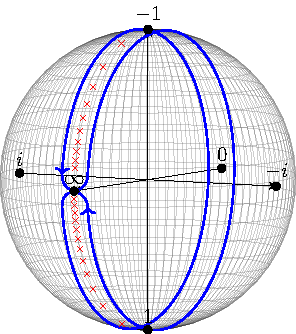
\includegraphics{thermal_field_theory/plots/integral_cont.pdf}        
    \end{subfigure}
    \begin{subfigure}{0.18\textwidth}
        \centering
        \begin{tikzpicture}
            \draw[-stealth] (0, 0) -- (1, 0);
        \end{tikzpicture}
        \end{subfigure}
    \begin{subfigure}{0.4\textwidth}
        \centering
        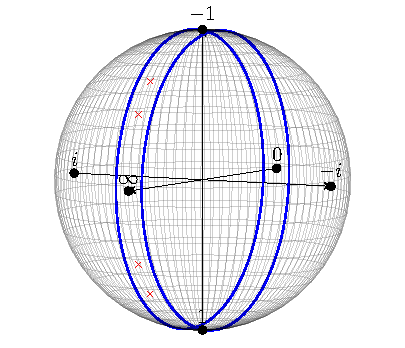
\includegraphics{thermal_field_theory/plots/integral_cont2.pdf}
    \end{subfigure} 
    \caption{The integral contour $\gamma$, and the result of deforming it into to contours close to the real line.
    The red crosses illustrate the poles of $n_B$.}
    \label{fig:integral contours}
\end{figure}
In the last line, we have changed variables $z \rightarrow -z$ in the first integral, and exploited the property $n_B(-i z) = -1 - n_B(iz)$.
As $n_B(iz)$ is analytic on the real line, the result is the sum of residues of $f$ in the lower half plane.
The function
\begin{equation}
    f(z) = \frac{1}{(z + i \mu)^2 + \omega^2} 
    = \frac{i}{2 \omega } 
    \left(
        \frac{1}{z + i(\mu + \omega)} - \frac{1}{z + i(\mu - \omega)}
    \right)
\end{equation}
obeys the assumed properties, as it has poles at
$z = - i (\mu \pm \omega)$, with residue $1 / 2 \omega$, so the function defined in \autoref{i func} may be written \footnote{Assuming $\omega>\mu$.}
\begin{equation}
    i(\omega, \mu) 
    % = \left(\frac{-2 \pi i^2}{2 \pi \omega}\right)
    % [1 + n_B(\omega + \mu) + n_B(\omega - \mu)].
    = \frac{1}{2\omega}
    [1 + n_B(\omega + \mu) + n_B(\omega - \mu)].
\end{equation}

Using the anti-derivative of the Bose distribution, we get the final form of \autoref{j func}
\begin{equation}
    j(\omega, \mu) = \int \dd \omega'\, \omega' i(\omega', \mu)
    =  
    \frac{1}{2}\omega + \frac{1}{2\beta} 
    \left[
        \ln\left(1 - e^{-\beta(\omega - \mu)}\right)
        + \ln\left(1 - e^{-\beta(\omega + \mu)}\right)
    \right]
    + g'(\beta).
\end{equation}
The extra $\omega$-independent term $g'(\beta)$ is an integration constant.
We see there are temperature dependent terms, one due to the particle and one due to the anti-particle, and one due to the antiparticle, as they have opposite chemical potentials.


\subsection{Regulating the free energy}
The free energy integral we obtained from the energy for the free scalar \autoref{free scalar free enrgy}, has two parts,
Noticing that the integral is spherically symmetric, we may write
\begin{equation}
    J_0 = \frac{1}{2} \int_{\tilde \Omega} \frac{\dd^3 k}{(2 \pi)^3} \sqrt{k^2 + m^2}, \quad
    J_T = \frac{1}{\beta} \int_{\tilde \Omega} \frac{\dd^3 k}{(2 \pi)^3} 
    \ln\left[1 - \exp(- \beta \sqrt{k^2 + m^2})\right], 
\end{equation}
The temperature-independent part, $J_0$, is clearly divergent, and we must therefore impose a regulator, and then add counter-terms.
This differs from the zero-temperature formalism, where there were no need to renormalize the free theory.
The second part of the integral, is convergent. 
To see this, we first exploit that it is spherically symmetric to write
\begin{equation}
    J_T = \frac{T^4}{2 \pi^2}\int_\R \dd x \, x^2  \ln(1 - e^{-\sqrt{x^2 + (\beta m)^2}}).
\end{equation}
Using the series expansion $\ln(1 + \epsilon) \sim \epsilon + \Oh{\epsilon}$, we can find the leading part of the  integrand for large $k$'s, 
\begin{equation}
    x^2 \ln(1 - e^{-\sqrt{x^2 + (\beta m)^2}}) \sim - x^2 e^{-x}, 
\end{equation}
which is suppressed exponentially, making the integral convergent.
In the limit of $T \rightarrow \infty$, we get
\begin{equation}
    J_\infty \sim \frac{T^4}{2 \pi^2} \int_\R \dd x \, x^2 \ln(1 - e^{-x})
    = - T^4 \frac{\pi^2}{90} = -\frac{3}{2} \sigma T^4,
\end{equation}
where $\sigma$ is the Stefan-Boltzmann constant. 

We use dimensional regularization on the temperature independent term. 
To that end, we define
\begin{equation}
    \Phi(m, d, A) = \int_{\tilde \Omega} \frac{\dd^d k}{(2 \pi)^d} (k^2 + m^2)^{-A},
\end{equation}
so that $J_0 = \Phi(m, 3, 1/2) / 2$.
Dimensional regularization takes uses the formula for integration of spherically symmetric function in $d$-dimensions,
\begin{equation}
    \int_{\R^d} \dd^d x \, f(r) 
    = \frac{2 \pi^{d/2}}{\Gamma(d/2)} \int_\R \dd r \, r^{d-1}f(r),
\end{equation}
where $r = \sqrt{x_i x_i}$ is the radial distance, and $\Gamma$ is the gamma-function.
The factor in the front of the integral comes from the solid-angle.
By extending this formula from integer-valued $d$ to real numbers, the function we defined becomes
\begin{equation}
    \Phi 
    = \frac{2 \pi^{d/2}}{\Gamma(d/2)} \int_\R \dd k \, 
    \frac{k^{d-1}}{(k^2 + m^2)^A}
    = \frac{m^{d - 2A}}{(4 \pi)^{d / 2}\Gamma(d/2)} 
    2 \int_\R \dd z \, \frac{z^{d - 1}}{(1 + z)^A}, 
\end{equation}
where we have made the change of variables $m z = k$.
We make one more change of variable to the integral,
\begin{equation}
    I = 2 \int_\R \dd z \, \frac{z^{d - 1}}{(1 + z)^A}
\end{equation}
Let
\begin{equation}
    z^2 = \frac{1}{s} - 1 \implies 2 z \dd z = - \frac{\dd s}{s^2}
\end{equation}
Thus,
\begin{equation}
    I = \int_0^a \dd s \, s^{A - d/2 - 1} (1 - z)^{d/2 - 1}.
\end{equation}
This is the beta-function, which can be written in terms of gamma-funcitons~\cite{Peskin:IntroQFT}
\begin{equation}
    I = B\left(A - \frac{d}{2}, \frac{d}{2}\right) 
    = \frac{\Gamma\left(A - \frac{d}{2}\right) \Gamma\left(\frac{d}{2}\right)}{\Gamma(A)}.
\end{equation}
Putting it all together, this gives
\begin{equation}
    \Phi = 
    \frac{
        (m^2)^{d/2 - A} \Gamma \left(A - \frac{d}{2} \right) 
    }
    {
        (4 \pi)^{d / 2}\Gamma(A)
    }.
\end{equation}
Inserting $d = 3 - 2\epsilon$ and $A = -1/2$, we get
\begin{equation}
    \frac{
        (m^2)^{3/2 - \epsilon - A} \Gamma \left(-2 + \epsilon \right) 
    }
    {
        (4 \pi)^{3/2 - \epsilon}\Gamma(-1/2)
    }
    = 
    \left(\frac{m^2}{4 \pi}\right)^{3/2} 
    \frac{m}{- 2 \pi^{1/2}}
    \mu^{-2\epsilon}
    \left(\frac{m^2}{4 \pi \mu^2}\right)^{- \epsilon}
    \frac{\Gamma(\epsilon)}{(\epsilon - 2)(\epsilon - 1)},
\end{equation}
where we have used the defining property $\Gamma(z + 1) = z\Gamma(z)$, and inserted a parameter $\mu$ with the dimensions of $m$.
Expanding around $\epsilon = 0$ gives
\begin{align}
    \left(\frac{m^2}{4 \pi \mu^2}\right)^{- \epsilon}
    &\sim 1 + \epsilon \ln\left(4 \pi \frac{\mu^2}{m^2}\right),\\
    \Gamma(\epsilon) 
    & \sim \frac{1}{\epsilon} - \gamma, \\
    \frac{1}{(\epsilon - 2)(\epsilon - 1)}
    &\sim \frac{1}{2}\left(1 + \frac{3}{2} \epsilon\right).
\end{align}
Inserting this back into the function gives
\begin{align}
    \Phi = 
    - \frac{m^4}{2^5 \pi^2} \mu^{-2 \epsilon}
    \left[1 + \epsilon \ln\left(4 \pi \frac{\mu^2}{m^2}\right)\right]
    \left(\frac{1}{\epsilon} - \gamma\right) \left(1 + \frac{3}{2} \epsilon\right)
    \sim
    - \frac{m^4}{2^5 \pi^2} \mu^{-2 \epsilon}
    \left[
        \frac{1}{\epsilon} 
        - \gamma + \frac{3}{2}
        + \ln\left(4 \pi \frac{\mu^2}{m^2}\right)
    \right].
\end{align}

\section{Interacting scalar}
\label{section:interacting scalar}

We now study a scalar field with a $\lambda \varphi^4$ interaction term.
We write the Lagrangian in the form
\begin{equation*}
    \Ell = \Ell^{(0)} + \Ell^{(I)}, \quad 
    \Ell^{(0)} = 
    \frac{1}{2} \partial_\mu \varphi \partial^\mu \varphi - m^2 \varphi^2 , \quad
    \Ell^{(I)} = - \frac{\lambda}{4!} \varphi^4
\end{equation*}
$\Ell^{(I)}$ is called the interaction term, and makes it impossible to exactly solve for the partition function.
Instead, we turn to perturbation theory.
The canonical partition function in this theory is
\begin{equation}
    Z = \Tr{e^{- \beta \hat H}}
    = \int_S \D \varphi \, \exp{
        - \int_\Omega \dd X \left(\Ell_E^{(0)} + \Ell_E^{(I)}\right)
    }
    = \int_S \D \varphi \, e^{-S_0} e^{-S_I}.
\end{equation}
Here, $S_0$ and $S_I$ denote the Euclidean action due to the free and interacting Lagrangian, respectively.
The domain of integration $S$ is again periodic field configurations $\varphi(\beta, \vec x) = \varphi(0, \vec x)$.
We may write the free energy as
\begin{equation*}
    - \beta F = \ln
    \left[
        \int_S \D \varphi \, e^{-S_0} \sum_n \frac{1}{n!} {(-S_I)}^n
    \right]
    = \ln Z_0 
    + \ln Z_I ,
\end{equation*}
where $Z_0$ is the partition function of the free theory.
The correction to the partition function is thus given by
\begin{equation}
    Z_I = \sum_{n=0}^\infty \frac{(-1)^n}{n!} \ex{{S_I}^n}_0,
\end{equation}
where
\begin{equation}
    \ex{A}_0 = \frac{
        \int_S \D \varphi \, A \, e^{-S_0} }
    {\int_S \D \varphi \, e^{-S_0}}.
\end{equation}

To evaluate expectation values of the form $\ex{\varphi(X_1) ... }_0$, we introduce the partition function with a source term
\begin{align}
    Z[J] = \int_S \D \varphi \, \exp{
        - \frac{1}{2} \int_\Omega \dd X \, \varphi (-\partial_E^2 + m^2) \varphi
        + \int_\Omega \dd X \, J \varphi
    }.
\end{align}

Thermal propagators are the generalization of the time-ordered two-point functions $\ex{T\{\varphi(x) \varphi(y) \}}$ of the vacuum formalism.
For some differential operator $D^{-1}$, the thermal propagator is defined as
\begin{equation}
    D^{-1} D(X, Y) = \beta \delta(X - Y).
\end{equation}
The Fourier transformed propagator is, assuming $D(X, Y) = D(X-Y, 0)$,
\begin{align}
    \nonumber
    \tilde D(K, K') 
    & = \frac{1}{V \beta^3} \int_{\Omega} \dd X \dd Y \, 
    D(X, Y) \exp(- i [X\cdot K + Y\cdot K']) \\ \nonumber
    & = \frac{1}{V \beta^3} \int_{\Omega} \dd X' \dd Y' \, D(X', 0) 
    \exp(- i [X'\cdot \frac{1}{2} (K - K') + Y\cdot (K + K')]) \\
    & = \frac{1}{V \beta^2} \tilde D(K) \delta(K + K'),
\end{align}
where
\begin{equation}
    \tilde D(K) = \int \dd X e^{iK\cdot X} D(X, 0).
\end{equation}
We write the thermal propagator of the free field as $D_0(X, Y)$.
With this, we may complete the square,
\begin{align}
    Z[J] = Z[0]\exp{\frac{1}{2} \int_{\Omega} \dd X \dd Y J(X) D_0(X, Y) J(Y)}
    = Z[0] \exp(W[J])
\end{align}
We can now write
\begin{equation}
    \ex{\varphi(X)\varphi(Y)}_0 
    = \frac{1}{Z[0]}
    \frac{\delta}{\delta J(X)} \frac{\delta}{\delta J(Y)} 
    Z[J] \Big|_{J=0} 
    = D_0(X, Y).
\end{equation}
This generalizes to higher order expectation values,
\begin{equation}
    \ex{\varphi(X_i) \dots \varphi(X_n)}_0
    = \frac{1}{Z[0hju]} \left(\prod_{i=1}^n \frac{\delta}{\delta J(X_i)}\right) 
    Z[J] \Big|_{J=0},
\end{equation}

Using Wick's theorem, as described in \autoref{section:path integral}, the expectation values we are evaluating can be written
\begin{align*}
    \ex{{S_I}^m}_0 & 
    = \left(- \frac{\lambda }{4!}\right)^m 
    \int_{\Omega} \dd X_1 \dots \dd X_m
    \ex{\varphi^4(X_1) \dots \varphi^4(X_m)}_0 \\ 
    & \quad
    = \left(- \frac{\lambda }{4!}\right)^m 
    \int_{\Omega} \dd X_1 \dots \dd X_m \sum_{\{a, b\}}
    \ex{\varphi(X_{a(1)}) \varphi(X_{b(1)})}_0
    \dots
    \ex{\varphi(X_{a(2m)}) \varphi(X_{b(2m)})}_0
\end{align*}
where $X_i$ for $i>m$ is defined to equal $X_j$, where $j = i \mod m$.
More simpliy,  $X_{m + i} = X_i$.
The functions $a,\,b$ represents a possible pairing, as described in \autoref{section:path integral}.
Inserting the Fourier expansions of the field gives
\begin{align*}
    & \ex{{S_I}^m}_0 \\
    &\quad 
    = \left(-\frac{\lambda }{4!}\right)^m 
    \int_{\Omega} \dd X_1 \dots \dd X_m
    (V \beta)^2 \int_{\tilde \Omega} \dd K_1 ... \dd K_{2m} \sum_{\{a, b\}} \\
    & \quad \quad \quad \quad\quad \quad \quad
    \ex{\varphi(K_{a(1)}) \varphi(K_{b(1)})}_0
    \dots
    \ex{\varphi(K_{a(2m)}) \varphi(K_{b(2m)})}_0     
    \exp(i {\sum}_{i=1}^{m} X_i \cdot K_i)\\ 
    & \quad  
    = \left(-\frac{\lambda }{4!}\right)^m 
    \frac{(V \beta)^{2m} \beta^m}{(V \beta^2)^{2m}}
    \int_{\tilde \Omega} \dd K_1 ... \dd K_{2m} \sum_{\{a, b\}} \\
    & \quad \quad \quad \quad \quad \quad \quad \quad \quad
    \tilde D(K_{a(1)}) \delta(K_{a(1)} + K_{b(1)}) \dots 
    \tilde D(K_{a(2m)}) \delta(K_{a(2m)} + K_{b(2m)})
    \prod_{i=1}^m \delta\left(X_i \cdot {\sum}_{j=0}^3 K_{i + jm}\right) \\
    & \quad 
    = \left(-\frac{\lambda \beta}{4!}\right)^m 
    \prod_{i=1}^{2m} \int_{\tilde \Omega} 
    \left( \dd K_i \frac{1}{\beta} \tilde D(K_i)  \right) 
    \prod_{i=1}^m \delta\left(X_i \cdot {\sum}_{j=0}^3 K_{i + jm}\right)
    \sum_{\{a, b\}} 
    \prod_{n=1}^{2m}\delta(K_{a(k)} + K_{b(k)}).
\end{align*}
Here we have used that $V \beta^2 \tilde D_0(K, P) = \tilde D_0(K) \delta(P + K)$, where $\tilde D_0(K)$ is the thermal propagator for the free field.
In this case, it is
\begin{equation}
    \tilde D_0(K) = \tilde D_0(\omega_n, \vec k) = \frac{1}{\omega_k^2 + \omega_n^2}.
\end{equation}
This expectation value can be represented graphically using Feynman diagrams.
The thermal $\lambda \varphi^2$-theory gets the prescription

\begin{align}
    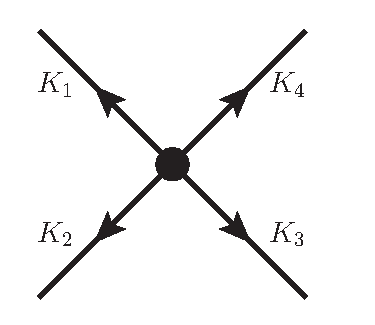
\includegraphics[width=0.15\textwidth, valign=c]{figurer/feynman-diagram/phi-4_vertex.eps}
    & = -\lambda \beta
    \delta \left({\sum}_i K_i \right), \\ \nonumber \\
    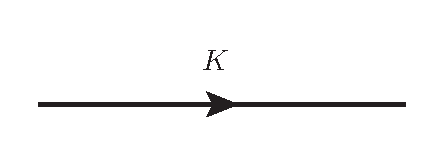
\includegraphics[width=0.2\textwidth, valign=c]{figurer/feynman-diagram/phi-4_propagator.eps}
    & = \frac{1}{\beta} D_0(K).
\end{align}
Lastly, one has to integrate over internal momenta and divide by the symmetry factor of the diagram $s$, which is described in detail in~\cite{Peskin:IntroQFT}.

Calculating $\ex{{S_I}^n}_0$ boils down to the sum of all possible Feynman diagrams with $n$ vertices.
The first example is 
\begin{align}
    \ex{S_I}_0 =
    \frac{1}{8} 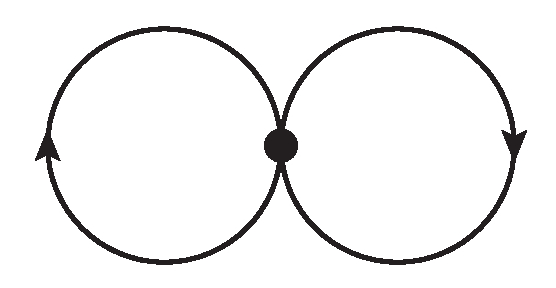
\includegraphics[width=0.15\textwidth, valign=c]{figurer/feynman-diagram/phi-4_loop_notext.eps}.
\end{align}

In \autoref{section:path integral}, we saw that the sum of all vacuum diagrams is the exponential of the sum of all \emph{connected} diagrams, so the free energy of the interacting theory is given by
\begin{equation}
    - \beta F = \ln Z_0 + \Sigma(\mathrm{all\,\, connected\,\, diagrams}).
\end{equation}

\section{Fermions}

The phase factor $e^{i\theta}$ that was introduced in \autoref{section:imaginary-time formalism} can be determined by studying the properties of the thermal Greens function.
The thermal Greens function may be written 
\begin{equation*}
    D(X_1, X_2) = D(\vec x, \vec y, \tau_1, \tau_2) 
    = \ex{e^{-\beta \hat H} \T{ \hat \varphi(X_1) \hat \varphi(X_2) } }.
\end{equation*}
$\T{...}$ is time-ordering operator,
% the temperature ordering operator, analogous to the time ordering operator from scattering theory.
and is defined as
\begin{equation*}
    \T{\varphi(\tau_1)\varphi(\tau_2)}
    = \theta(\tau_1 - \tau_2) \varphi(\tau_1)\varphi(\tau_2)
    + \nu \theta(\tau_2 - \tau_1) \varphi(\tau_2)\varphi(\tau_1),
\end{equation*}
where $\nu = \pm 1$ for bosons and fermions respectively, and $\theta(\tau)$ is the Heaviside step function.
In the same way that $i \hat H$ generates the time translation of a quantum field operator through $\hat\varphi(x) = \hat\varphi(t, \vec x) = e^{it\hat H} \hat \varphi(0, \vec x) e^{-it\hat H} $, the imaginary-time formalism implies the relation
\begin{equation}
    \hat\varphi(X) = \hat\varphi(\tau, \vec x) 
    = e^{\tau\hat H} \hat \varphi(0, \vec x) e^{-\tau \hat H}.
\end{equation}
Using $\one = e^{\tau \hat H} e^{-\tau \hat H}$ and the cyclic property of the trace, we show that, assuming $\beta>\tau>0$,
\begin{align*}
    G(\vec x, \vec y, \tau, 0)
    & = \ex{e^{-\beta \hat H} \T{\varphi(\tau, \vec x) \varphi(0, \vec y)}} \\
    & = \frac{1}{Z} \Tr{
        e^{-\beta \hat H} \varphi(\tau, \vec x) \varphi(0, \vec y)
    } \\
    & = \frac{1}{Z} \Tr{
        \varphi(0, \vec y) e^{-\beta \hat H} \varphi(\tau, \vec x)
    } \\
    & = \frac{1}{Z} \Tr{
        e^{-\beta \hat H} e^{\beta \hat H} \varphi(0, \vec y) 
        e^{-\beta \hat H} \varphi(\tau, \vec x)
    } \\
    & = \frac{1}{Z} \Tr{
        e^{-\beta \hat H} \varphi(\vec y, \beta) \varphi(\tau, \vec x)
    } \\
    & = \nu \ex{
        e^{-\beta \hat H} \T{ \varphi(\tau, \vec x) \varphi( \beta, \vec y) }
    }.
\end{align*}
This implies that $\varphi(0, x) = \nu \varphi(\beta, \varphi)$, which shows that bosons are periodic in time, as stated earlier, while fermions are anti-periodic.

The Lagrangian density of a free fermion is
\begin{equation}
    \Ell = \bar \psi \left( i \slashed{\partial} - m \right) \psi.
\end{equation}
This Lagrangian is invariant under the transformation $\psi \rightarrow e^{-i \alpha} \psi$, which by Nöther's theorem results in a conserved current
\begin{equation}
    j^\mu = \pdv{\Ell}{(\partial_\mu \psi)} \delta \psi=  \bar \psi \gamma^\mu \psi.
\end{equation}
The corresponding conserved charge is 
\begin{equation}
    Q = \int_V \dd^3 x\, j^0 = \int_V \dd^3 x \, \bar \psi \gamma^0 \psi.
\end{equation}
We can now use our earlier result for the thermal partition function, \autoref{Thermal partition function}, only with the substitution $\He \rightarrow \He - \mu \bar \psi \gamma^0 \psi$, and integrate over anti-periodic $\psi$'s:
\begin{equation*}
    Z = \Tr{e^{-\beta(\hat H - \mu \hat Q)}}
    = \prod_{a b}\int \D \psi_a\D \pi_b \exp{
        \int_{\Omega} \dd X \, 
        \left(
            i\dot \psi \pi - \He(\psi, \pi) + \mu \bar \psi \gamma^0 \psi
        \right)
    },
\end{equation*}
where $a, b$ are the spinor indices.
The canonical momentum corresponding to $\psi$ is
\begin{equation}
    \pi = \pdv{\Ell}{(\partial_0 \psi)} = i \bar \psi \gamma^0,
\end{equation}
and the Hamiltonian density is 
\begin{equation}
    \He = \pi \dot\psi - \Ell
    = \bar \psi (-i\gamma^i\partial_i + m) \psi
\end{equation}
which gives
\begin{equation}
    \Ell_E = 
    - i \pi \dot\psi + \He(\psi, \pi) - \mu \bar \psi \gamma^0 \psi
    = \bar\psi[\gamma^0 (\partial_\tau - \mu) - i\gamma^i \partial_i + m] \psi,
\end{equation}
By using the Grassman-version of the Gaussian integral formula, the partition function can be written
\begin{align*}
    Z & = \prod_{a b}\int \D \psi_a\D \bar \psi_b 
    \exp{
        - \int_\Omega \dd X \, \bar \psi
        \left[
            \tilde\gamma_0(\partial_\tau -\mu) -  i \gamma^i \partial_i + m
        \right]
        \psi
    }\\
    & = C \prod_{a b}\int \D \tilde \psi_a\D \tilde {\bar \psi}_b 
    \exp{
        - \int_{\tilde \Omega} \dd K \, \tilde {\bar \psi}
        \left[
            i \tilde\gamma_0(\omega_n + i\mu) + i \gamma_i p_i + m
        \right]
        \tilde \psi
    } \\
    & = C \prod_{a b}\int \D \tilde \psi_a\D \tilde {\bar \psi}_b 
    e^{- \langle \tilde {\bar \psi}, D_0^{-1} \psi\rangle} 
    = \det(D_0^{-1}).
\end{align*}
In the second line, we have inserted the Fourier expansion of the field, as defined in \autoref{Conventions and notation}, and changed variable of integration, as we did for the scalar field.
The linear operator in this case is 
\begin{equation}
    D_0^{-1} = i \gamma^0 (-i\partial_\tau + i\mu) - (- i \gamma^i) \partial_i + m
    = 
    \beta [i \tilde \gamma_a p_a + m ].
\end{equation}
This equality must be understood as an equality between linear operators, which are represented in different bases.
We introduced the notation $p_{n;a} = (\omega_n + i \mu, p_i)$ and use the Euclidean gamma matrices, as defined in \autoref{Conventions and notation}.
We use the fact that 
\begin{equation*}
    \det(i\tilde\gamma_a p_a + m)
    = \det(\gamma^5 \gamma^5)
    \det(i\tilde\gamma_a p_a + m)
    = \det[\gamma^5 (i\tilde\gamma_a p_a + m) \gamma^5]
    = \det(-i\tilde\gamma_a p_a + m),
\end{equation*}
Let $\tilde D = -i\tilde\gamma_a p_a + m$, which means we can write
\begin{equation}
    Z = \sqrt{\det(D)\det(\tilde D)} = \sqrt{\det(D\tilde D)} = \det[\one(p_a p_a + m^2)]^{1/2},
\end{equation}
where we have used the anti-commutation rule for the Euclidean gamma-matrices, $\acom{\gamma_a}{\gamma_b} = 2 \delta_{ab}$.
It is important to keep in mind that the determinant here refers to linear operators on the space of spinor functions.
\begin{align}
    \nonumber
    \ln(Z) & = \ln\left\{\det[\one(p_a p_a + m^2)]^{1/2}\right\}
    = \frac{1}{2} \Tr{\ln[\one(p_a p_a + m^2)]} \\
    & = \frac{1}{2} \int_{\tilde \Omega} \dd K \ln[\one \beta^2 (p_a p_a + m^2)]_{aa}
\end{align}
As the matrix within the logarithm is diagonal, the matrix-part of the trace is trivial, and the free energy may be written
\begin{equation}
    \beta \Ef
    = - 2 \int_{\tilde \Omega} \dd X \,  \ln\{ \beta^2[(\omega_n + i\mu)^2 + \omega_k^2]\} .
\end{equation}
Using the fermionic version of the thermal sum from \autoref{section:thermal sum} gives the answer
\begin{equation}
    \Ef = 2 \int\frac{\dd^3 p}{(2\pi)^3} \, 
    \left[
        \beta \omega_k
        + \frac{1}{\beta} \ln\left(1 + e^{-\beta(\omega_k-\mu)}\right)
        + \frac{1}{\beta} \ln\left(1 + e^{-\beta(\omega_k+\mu)}\right)
    \right].
\end{equation}
We see again that the temperature-independent part of the integral diverges, and must be regulated.
There are two temperature-dependent terms, one from the particle and one from the anti-particle.


% \chapter{Appendices}

\chapter{Algebra bases}
\label{section:algebra bases}

\subsection*{Pauli matrices}
The $\liea{su}{2}$ basis used is the Pauli matrices,
\begin{align}
    \tau_1 = 
    \begin{pmatrix}
        0 & 1 \\
        1 & 0 \\
    \end{pmatrix}
    , \quad 
    \tau_2 = 
    \begin{pmatrix}
        0 & -i \\
        i & 0 \\
    \end{pmatrix}, \quad 
    \tau_3 = 
    \begin{pmatrix}
        1 & 0 \\
        0 & -1 \\
    \end{pmatrix}.
\end{align}
They obey
\begin{align}
    \com{\tau_a}{\tau_b} &= 2 i \eps_{abc}\tau_c, \\
    \acom{\tau_a}{\tau_b} &= 2\delta_{ab} \one, \\
    \quad \Tr{\tau_a} &= 0, \\
    \quad \Tr{\tau_a \tau_b} &= 2 \delta_{ab}.
\end{align}
Together with the identity matrix $\one$, the Pauli matrices form a basis for the vector space of all 2-by-2 matrices.
An arbitrary 2-by-2 matrix $M$ may be written
\begin{equation}
    \label{2-by-2 matrix decomp}
    M = M_0 \one + M_a \tau_a, \quad 
    M_0 = \frac{1}{2} \Tr{M}, \,\, M_a = \frac{1}{2} \Tr{\tau_a M}.
\end{equation}


\subsection*{Gamma matrices}

The gamma matrices $\gamma^\mu$, $\mu \in \{0, 1, 2, 3\}$, obey
\begin{gather}
    \acom{\gamma^\mu}{\gamma^\nu} = 2 g^{\mu \nu} \one,\\
    {\gamma^0}^\dagger = \gamma^0, \quad {\gamma^i}^\dagger = - \gamma^i.
\end{gather}
These matrices, together with
\begin{align}
    \sigma^{\mu\nu} &= \frac{1}{2} [\gamma^\mu, \gamma^\mu], \\ 
    \gamma_A^\mu &= \gamma^\mu \gamma^5, \\
     \gamma^5 
    &= \frac{i}{4!}\epsilon_{\mu \nu \rho \sigma} \gamma^{\mu}\gamma^{\nu}\gamma^{\rho}\gamma^{\sigma},
\end{align}
form the Clifford algebra $\text{Cl}_{1,3}$, also known as the \emph{space-time algebra}.
The subscripts $(1, 3)$ denotes the signature of the metric.
The ``fifth $\gamma$-matrix'', which can be expressed as $\gamma^5 = \gamma^0\gamma^1\gamma^2\gamma^3$, obey
\begin{equation}
    \acom{\gamma^5}{\gamma^\mu} = 0, \quad (\gamma^5)^2 = \one.
\end{equation}


The Euclidian counterpart of the space-time algebra, $\text{Cl}_4$, is defined by the ``Euclidian gamma matrices'', which obey
\begin{equation}
    \acom{\tilde \gamma_a}{\tilde \gamma_b} = 2 \delta_{ab}\one.
\end{equation}
These can be related to the regular Minkowski-matrices by
\begin{equation}
    \tilde \gamma_0 = \gamma^0,\quad 
    \tilde \gamma_j = -i\gamma^j.
\end{equation}
These then obey
\begin{equation}
    {\tilde\gamma_a}^\dagger = \tilde\gamma_a.
\end{equation}
The Euclidean $\tilde \gamma_5$ is defined as
\begin{equation}
    \tilde \gamma_5 = \gamma_0\gamma_1\gamma_2\gamma_3 = i \gamma^0\gamma^1\gamma^2\gamma^3 = \gamma^5.
\end{equation}
It thus also anti-commutes with the Euclidean $\gamma$-matrices,
\begin{equation}
    \{\tilde \gamma_5, \tilde \gamma_a\} = 0.
\end{equation}

\chapter{Functional derivatives}
\label{section:Functional derivative}

Functional derivatives generalize the notion of gradients and directional derivatives.
A function $f(x)$ has a gradient
\begin{equation}
    \dd f_{x_0} = \pdv{f}{x_i} \Big|_{x_0} \dd x_i.
\end{equation}
The derivative in a particular direction $v = v^i \partial_i$ is 
\begin{equation}
    \dv{\epsilon} f(x_i + \epsilon v_i) \Big|_{\epsilon = 0} 
    = f(x) + \dd f_x (v) = f(x) + \pdv{f}{x^i}v_i.
\end{equation}
This is generalized to functionals through the definition of the functional derivative and the variation of a functional.
Let $F[f]$ be a functional, i.e., a machine that takes in a function and returns a number or a function.
The obvious example in our case is the action, which takes in one or more field configurations, and returns a single real number.
We will assume here that the functions have the domain $\Omega$, with coordinates $x$.
The functional derivative is defined as
\begin{equation}
    \delta F[f]
    =
    \dv{\epsilon} F[f + \epsilon \eta] \Big|_{\epsilon = 0}
    = \int_\Omega \dd x \, \frac{\delta F[f]}{\delta f(x)} \eta(x).
\end{equation}
$\eta(x)$ is here an arbitrary function, but we will make the assumption that it as well as all its derivatives are zero at the boundary of its domain $\Omega$, i.e., $\eta(\partial \Omega) = 0$.
This allows us to discard surface terms stemming from partial integration, which we will use frequently.
We may use the definition to derive one of the fundamental relations of functional derivation.
Take the functional $F[f] = f(x)$. 
Then,
\begin{equation}
    \label{Functional derivative delta identity}
    \delta F[f] = \dv{\epsilon} [f(x) + \epsilon \eta(x)] \Big|_{\epsilon = 0}
    = \eta(x) = \int \dd y \, \delta(x - y) \eta(y)
\end{equation}
This leads to the identity
\begin{equation}
    \frac{\delta f(x)}{\delta f(y)} = \delta(x - y),
\end{equation}
for any function $f$.
Higher functional derivatives are defined similarly, by applying functional variation repeatedly
\begin{equation}
    \delta^n F[f] = \dv{\epsilon} \delta^{n-1}F[f + \epsilon \eta_n] \big|_{\epsilon=0}
    = \int \left(\prod_{i=1}^n \dd x_i\right)
    \frac{\delta^n F[f]}{ \delta f(x_n)\dots\delta f(x_1)} \left(\prod_{i=1}^n \eta_i(x_i)\right).
\end{equation}
If we can write the functional $F[f]$ in terms of a new variable, $g(y)$, then the chain rule for functional derivatives is
\begin{equation}
    \fdiff{F[f]}{f(x)} = \int \dd y \, \fdiff{F[f]}{g(y)} \fdiff{g(y)}{f(x)}.
\end{equation}

A functional may be expanded in a generalization of the Taylor series, 
\begin{equation}
    F[f_0 + f] = F[f_0] + \int_\Omega \dd x \, f(x) \frac{\delta F[f_0]}{\delta f(x)}
    + \frac{1}{2!}\int_\Omega \dd x \dd y \, f(x) f(y) \frac{\delta^2 F [f_0]}{\delta f(x) \delta f(y)}
    + \dots
\end{equation}
Her, the notation
\begin{equation}
    \fdiff{F[f_0]}{f(x)}
\end{equation}
indicate that the functional $F[f]$ is first differentiated with respect to $f$, the evaluated at $f = f_0$.
As an example, the Klein-Gorodn action
\begin{equation}
    S[\varphi] = - \frac{1}{2}\int_\Omega \dd x \, \varphi(x) (\partial^2 + m^2) \varphi(x).
\end{equation}
Using \autoref{Functional derivative delta identity} and partial integration,
\begin{align}
    \nonumber
    \funcdv{\varphi(x)} S[\varphi] 
    & = 
    - \frac{1}{2} \int_\Omega \dd y \, 
    [\delta(x - y)(\partial_y^2 + m^2)\varphi(y) + \varphi(y) (\partial_y^2 + m^2)\delta(x - y)] \\
    & = 
    - \int_\Omega \dd y \, 
    \delta(x - y)(\partial_y^2 + m^2)\varphi(y) 
    = (\partial_x^2 + m^2)\varphi(x)
\end{align}
The second derivative is
\begin{equation}
    \frac{\delta^2S[\varphi]}{\delta \varphi(x)\delta \varphi(y)}
    =
    \funcdv{\varphi(x)} (\partial_y^2 + m^2)\varphi(y)
    = 
    (\partial_y^2 + m^2) \delta(x - y).
\end{equation}


\subsection*{Gaussian integrals}
\label{section:gaussian integrals}

\begin{figure}[ht]
    \centering
    \begin{tikzpicture}
        \draw (-2, 0) -- (2, 0) node[right] {$\mathrm{Re}(x)$};
        \draw (0, -2) -- (0, 2) node[above] {$\mathrm{Im}(x)$};
        \draw[->, thick] (-1.75, 0.1) -- (1.8, 0.1);
        \draw[->, thick] (1.8, 0.15) arc (10:45:1.8);
        \draw[->, thick] ({1.8/sqrt(2)}, {1.8/sqrt(2)}) -- ({-1.8/sqrt(2)}, {-1.8/sqrt(2)});
        \draw[->, thick] ({-1.8/sqrt(2)}, {-1.8/sqrt(2)}) arc (225:180:1.8);
    \end{tikzpicture}
    \caption{Wick rotation}
    \label{Wick rotation}
\end{figure}


A useful integral is the Gaussian integral,
\begin{equation}
    \int_\R \dd x \, \exp(- \frac{1}{2} a x^2) = \sqrt{\frac{2 \pi}{a}},
\end{equation}
for $a \in \R$. The imaginary version,
\begin{equation}
    \int_R \dd x \, \exp(i \frac{1}{2} a x^2 )
\end{equation}
does not converge. However, if we change $a \rightarrow a + i\epsilon$, the integrand is exponentially suppressed.
\begin{equation}
    f(x) = \exp(i \frac{1}{2}a x^2) \rightarrow
    \exp(i\frac{1}{2}a x^2 - \frac{1}{2} \epsilon  x^2).
\end{equation}
As the integrand falls exponentially for $x\rightarrow \infty$ and contains no poles in the upper right nor lower left quarter of the complex plane, we may perform a wick rotation by closing the contour as shown in \autoref{Wick rotation}.
This gives the result
\begin{equation}
    \label{complex gauss 1D}
    \int_\R \dd x \, \exp(i \frac{1}{2}(a + i\epsilon) x^2) 
    = \int_{\sqrt{i}\R} \dd x \, \exp(i\frac{1}{2} ax^2)
    = \sqrt{i} \int_\R \dd y\, \exp(-\frac{1}{2} (-a) y^2) = \sqrt{\frac{2 \pi i}{(-a)}}
\end{equation}
where we have made the change of variable $y = (1+i)/\sqrt{2} x = \sqrt{i} x$.
In $n$ dimensions, the Gaussian integral formula generalizes to
\begin{equation}
    \int_{\R^n} \dd^n x \, \exp{-\frac{1}{2} x_n A_{nm} x_m } =\sqrt{\frac{(2 \pi)^n}{\det(A)}},
\end{equation}
where $A$ is a matrix with $n$ real, positive eigenvalues.
We may also generalize \autoref{complex gauss 1D},
\begin{align}
    \int_{\R^n} \dd^n x \, \exp{i\frac{1}{2} x_n( A_{nm} + i \epsilon \delta_{nm}) x_m } =\sqrt{\frac{(2 \pi i )^n}{\det(-A)}}.
\end{align}
The final generalization is to functional integrals,
\begin{align}
    \int \D \varphi \, \exp(- \frac{1}{2} \int \dd x \, \varphi(x) A \varphi(x) )
    = C (\det(A))^{-1/2},
    \int \D \varphi \, \exp(i\frac{1}{2} \int \dd x \, \varphi(x) A \varphi(x) )
    = C (\det(-A))^{-1/2}.
\end{align}
$C$ is here a divergent constant, but will either fall away as we are only looking at the logarithm of $I_\infty$ and are able to throw away additive constants, or ratios between quantities which are both multiplied by $C$.

The Gaussian integral can be used for the stationary phase approximation.
In one dimension, it is
\begin{equation}
    \int \dd x \, \exp{i \alpha f(x)} 
    \approx \sqrt{\frac{2 \pi }{f''(x_0)}}\exp{ f(x_0)}, 
    \, \alpha\rightarrow \infty,
\end{equation}
where the point $x_0$ is defined by $ f'(x_0) = 0$. 
The functional generalization of this is
\begin{equation}
    \int \D \varphi \exp{i S[\varphi]}
    \approx 
    C \det(- \frac{\delta^2 S[\varphi_0]}{\delta \varphi^2})
    \exp{i \alpha S[\varphi_0]  },
\end{equation}
Here, $S[\varphi]$ is a general functional of $\varphi$, we have used the Taylor expansion, and $\varphi_0$ obeys
\begin{equation}
    \funcdv{\varphi(x)}{S[\varphi_0]} = 0.
\end{equation}


\chapter{Rewriting terms}
\label{appendix:rewriting terms}

In this section, we will show how to rewrite terms in the Lagrangian of Chiral perturbation theory.
These techniques, and more, are used to reduce the total number of terms, and change between different conventions.

\subsection*{Equation of motion and redundant terms}

Changing the field parametrization that appears in the Lagrangian does not affect any of the physics, as it corresponds to a change of variables in the path integral~\cite{Scherer2002IntroductionTC,Chisholm:changeOfVar,Kamefuchi:changeOfVar}.
However, a change of variables can result in new terms in the Lagrangian.
As a result of this, terms that appear independent on the face of it may be redundant.
These terms can be eliminated by using the classical equation of motion.
In this section, we show first the derivation of the equation of motion, then use this result to identify redundant terms which need not be included in the most general Lagrangian.

We derive the equation of motion for the leading order Lagrangian using the principle of least action.
Choosing the parametrization $\Sigma = \exp(i \pi_a \tau_a)$, a variation $\pi_a \rightarrow \pi_a + \delta \pi_a$ results in a variation in $\Sigma$, $\delta \Sigma = i \tau_a \delta \pi_a \Sigma $.
The variation of the leading order action,
\begin{equation}
    S_2 = \int_\Omega \dd^4x \, \Ell_2,
\end{equation}
when varying $\pi_a$ is 
\begin{align*}
    \delta S = \int_\Omega \dd x \, \frac{f^2}{4}
    \Tr{
        (\nabla_\mu \delta \Sigma) (\nabla^\mu \Sigma)^\dagger
        + (\nabla_\mu \Sigma) (\nabla^\mu \delta \Sigma)^\dagger
        + \chi \delta \Sigma^\dagger + \delta \Sigma \chi^\dagger
    }.
\end{align*}
Using the properties of the covariant derivative to do partial integration, as show in \autoref{Covarinat derivative}, as well as $\delta(\Sigma \Sigma^\dagger) = (\delta\Sigma)\Sigma^\dagger + \Sigma (\delta \Sigma)^\dagger = 0$, the variation of the action can be written
\begin{align*}
    \delta S 
    & = \frac{f^2}{4} \int_\Omega \dd x\, 
    \Tr{
        - \delta \Sigma \nabla^2 \Sigma^\dagger
        + (\nabla^2 \Sigma) (\Sigma^\dagger \delta \Sigma \Sigma^\dagger)
        - \chi (\Sigma^\dagger \delta \Sigma \Sigma^\dagger)
        + \delta \Sigma \chi^\dagger
    } \\
    & = 
    \frac{f^2}{4} \int_\Omega \dd x\, 
    \Tr{
        \delta \Sigma \Sigma^\dagger 
        \left[
            (\nabla^2 \Sigma)\Sigma^\dagger
            - \Sigma \nabla^2 \Sigma^\dagger
            - \chi \Sigma^\dagger
            + \Sigma \chi^\dagger
        \right]
        } \\
    & = 
    i \frac{f^2}{4} \int_\Omega \dd x\, 
    \Tr{\tau_a 
    \left[
         (\nabla^2 \Sigma)\Sigma^\dagger
        - \Sigma \nabla^2 \Sigma^\dagger
        - \chi \Sigma^\dagger
        + \Sigma \chi^\dagger
    \right]
    } 
    \delta \pi_a = 0.
\end{align*}  
As the variation is arbitrary, the equation of motion to leading order is
\begin{equation}
    \Tr{
        \tau_a 
        \left[
            (\nabla^2 \Sigma)\Sigma^\dagger
            - \Sigma \nabla^2 \Sigma^\dagger
            - \chi \Sigma^\dagger
            + \Sigma \chi^\dagger
        \right]
    } = 0.
\end{equation}
We define
\begin{equation}
    \mathcal O_\text{EOM}^{(2)}
    = 
    (\nabla^2 \Sigma)\Sigma^\dagger
    - \Sigma \nabla^2 \Sigma^\dagger
    - \chi \Sigma^\dagger
    + \Sigma \chi^\dagger.
\end{equation}


The next step in eliminating redundant terms is to change the parametrization of $\Sigma$ by $\Sigma(x) \rightarrow \Sigma'(x)$.
Here, $ \Sigma(x) = e^{iS(x)} \Sigma'(x), \, S(x) \in \liea{su}{2}$. This change leads to a new Lagrange density, $\Ell[\Sigma] = \Ell[\Sigma'] + \Delta \Ell[\Sigma']$.
We are free to choose $S(x)$, as long $\Sigma'$ still obeys the required transformation properties.
Any terms in the Lagrangian $\Delta \Ell$ due to a reparametrization can be neglected, as argued earlier.
When demanding that $\Sigma'$ obey the same symmetries as $\Sigma$,
the most general transformation to second order in Weinberg's power counting scheme  is~\cite{Scherer2002IntroductionTC}
\begin{equation}
    \label{S reparametrization}
    S_{2} = 
    i \alpha_2 
    \left[
        (\nabla^2 \Sigma') \Sigma^\dagger - \Sigma' (\nabla^2 {\Sigma'})^\dagger
    \right]
    + i \alpha_2
    \left[
        \chi \Sigma'^\dagger - \Sigma' \chi^\dagger 
        - \frac{1}{2} \Tr{\chi \Sigma'^\dagger - \Sigma' \chi^\dagger}
    \right].
\end{equation}
$\alpha_1$ and $\alpha_2$ are arbitrary real numbers. As \cref{S reparametrization} is to second order, $\Delta \Ell$ is fourth order in Weinberg's power counting scheme.
To leading order is given by
\begin{align*}
    \Ell_2\left[e^{i S_2}\Sigma '\right]
    & =
    \frac{f^2}{4}\Tr{[\nabla_\mu (1 +i S_2)\Sigma'][\nabla^\mu \Sigma'^\dagger  (1 - i S_2)]}
    + \frac{f^2}{4} \Tr{\chi\Sigma'^\dagger (1 - i S_2) + (1 +i S_2)\Sigma' \chi^\dagger} \\
    & = \Ell[\Sigma'] + 
    i \frac{f^2}{4}
    \Tr{[\nabla_\mu (S_2\Sigma')][\nabla^\mu\Sigma']^\dagger 
    -  [\nabla_\mu\Sigma'][\nabla^\mu (\Sigma'^\dagger  S_2) ]}
    - i \frac{f^2}{4} \Tr{\chi \Sigma'^\dagger S_2 - S_2 \Sigma' \chi^\dagger}
\end{align*}
Using the properties of the covariant derivative, we may use the product rule and partial integration to write the difference between the two Lagrangians to fourth-order as
\begin{align}
    \nonumber
    \Delta \Ell[\Sigma'] 
    & = 
    i \frac{f^2}{4}
    \Tr{
        (\nabla_\mu S_2)
        (\Sigma' \nabla^\mu \Sigma'^\dagger - (\nabla^\mu \Sigma') \Sigma'^\dagger) 
    }
    - i \frac{f^2}{4} \Tr{\chi \Sigma'^\dagger  S_2 - S_2 \Sigma' \chi^\dagger} \\
    & = 
    \label{Delta reparametrization}
    \frac{f^2}{4} \Tr{i S_2 \mathcal{O}_\mathrm{EOM}^{(2)}}.
\end{align}
Any term that can be written in the form of \cref{Delta reparametrization} for arbitrary $\alpha_1, \alpha_2 \in \R$ is redundant, as we argued earlier, and may therefore be discarded.
$\Delta \Ell_2$ is of fourth order, and it can thus be used to remove terms from $\Ell_4$ or higher order.


\subsection*{Rewriting NLO Lagrangian}
\label{subsection:rewriting NLO Lagrangian}

The NLO Lagrangian used in this text is given in \cref{NLO Lagrangian}, and is
\begin{align}
    \notag
    \Ell_4 
    & = 
    \frac{l_1}{4} \Tr{\nabla_\mu \Sigma (\nabla^\mu \Sigma)^\dagger}^2
    + \frac{l_2}{4} \Tr{\nabla_\mu \Sigma (\nabla_\nu \Sigma)^\dagger} 
    \Tr{\nabla^\mu \Sigma (\nabla^\nu \Sigma)^\dagger} 
    +
    \frac{l_3 + l_4}{16} \Tr{\chi \Sigma^\dagger + \Sigma \chi^\dagger}^2
    \\ \notag
    &
    + \frac{l_4}{8}\Tr{\nabla_\mu \Sigma (\nabla^\mu \Sigma)^\dagger} \Tr{\chi \Sigma^\dagger + \Sigma \chi^\dagger}
    - \frac{l_7}{16} \Tr{\chi \Sigma^\dagger - \Sigma \chi^\dagger}^2
    + \frac{h_1 + h_3 - l_4}{4} \Tr{\chi \chi^\dagger} \\
    & +
    \frac{h_1 - h_3 - l_4}{16}
    \left[
        \Tr{\chi \Sigma^\dagger + \Sigma \chi^\dagger}^2
        + \Tr{\chi \Sigma^\dagger - \Sigma \chi^\dagger}^2
        -2 \Tr{\left(\chi \Sigma^\dagger\right)^2 + \left( \Sigma \chi^\dagger\right)^2}
    \right].
\end{align}
We can rewrite it to match the one used in~\cite{Andersen:two-flavor-chpt,mojahed}, starting with
\begin{align*}
    & \frac{h_1 - h_3 - l_4}{16}
    \left(
        \Tr{\chi \Sigma^\dagger - \Sigma \chi^\dagger}^2
        - 2 \Tr{(\chi \Sigma^\dagger)^2 + (\Sigma \chi^\dagger)^2}
    \right) \\
    & = 
    \frac{h_1 - h_3 - l_4}{16}
    \left(
        \Tr{\chi \Sigma^\dagger}^2 - 2\Tr{\chi \Sigma^\dagger}\Tr{\Sigma \chi^\dagger}
        + \Tr{\Sigma \chi^\dagger}^2
        - 2 \Tr{(\chi \Sigma^\dagger)^2} -2 \Tr{(\Sigma \chi^\dagger)^2}
    \right)
\end{align*}
Using $\Tr{A^2} = \Tr{A}^2 - \det(A)\Tr{\one}$, we get
\begin{align*}
    &= - \frac{h_1 - h_3 - l_4}{16}
    \left(
        \Tr{\chi \Sigma^\dagger}^2 + 2\Tr{\chi \Sigma^\dagger}\Tr{\Sigma \chi^\dagger}
        + \Tr{\Sigma \chi^\dagger}^2
        - 4 \det(\chi \Sigma^\dagger)
        - 4 \det(\Sigma\chi^\dagger)
    \right) \\
    &= - \frac{h_1 - h_3 - l_4}{16}
    \left(
        \Tr{\chi \Sigma^\dagger + \Sigma \chi^\dagger}^2
        - 4 \det(\chi \Sigma^\dagger)
        - 4 \det(\Sigma\chi^\dagger)
    \right)
\end{align*}
Furthermore, as $\det(\Sigma)= 1$, 
% and $\chi = a_i \tau_i$, we have $\Tr{\chi \chi^\dagger} = a_i a_i^*$, $\det(\chi) + \det(\chi^\dagger) = a_i a_i + a_i^* a_i^*$
\begin{align}
    \notag
    \Ell_4 
    & = 
    \frac{l_1}{4} \Tr{\nabla_\mu \Sigma (\nabla^\mu \Sigma)^\dagger}^2
    + \frac{l_2}{4} \Tr{\nabla_\mu \Sigma (\nabla_\nu \Sigma)^\dagger} 
    \Tr{\nabla^\mu \Sigma (\nabla^\nu \Sigma)^\dagger} 
    +
    \frac{l_3 + l_4 }{16} \Tr{\chi \Sigma^\dagger + \Sigma \chi^\dagger}^2
    \\\notag
    &
    + \frac{l_4}{8}\Tr{\nabla_\mu \Sigma (\nabla^\mu \Sigma)^\dagger} \Tr{\chi \Sigma^\dagger + \Sigma \chi^\dagger}
    - \frac{l_7}{16} \Tr{\chi \Sigma^\dagger - \Sigma \chi^\dagger}^2
    + \frac{h_1 + h_3 -l_4}{4} \Tr{\chi \chi^\dagger} \\
    & +\frac{h_1 - h_3 - l_4}{4} (\det{\chi} + \det{\chi^\dagger})
\end{align}
For real $\chi$, we have $\Tr{\chi \chi^\dagger} = \det(\chi) + \det(\chi^\dagger)$, and we can define $h_1' = h_1 - l_4$ to get
\begin{align}
    \notag
    \Ell_4 
    & = 
    \frac{l_1}{4} \Tr{\nabla_\mu \Sigma (\nabla^\mu \Sigma)^\dagger}^2
    + \frac{l_2}{4} \Tr{\nabla_\mu \Sigma (\nabla_\nu \Sigma)^\dagger} 
    \Tr{\nabla^\mu \Sigma (\nabla^\nu \Sigma)^\dagger} 
    +
    \frac{l_3 + l_4 }{16} \Tr{\chi \Sigma^\dagger + \Sigma \chi^\dagger}^2
    \\
    &
    + \frac{l_4}{8}\Tr{\nabla_\mu \Sigma (\nabla^\mu \Sigma)^\dagger} \Tr{\chi \Sigma^\dagger + \Sigma \chi^\dagger}
    - \frac{l_7}{16} \Tr{\chi \Sigma^\dagger - \Sigma \chi^\dagger}^2
    + \frac{h_1'}{2} \Tr{\chi \chi^\dagger}
\end{align}
If one assumes $\delta m = 0$, i.e., what is called the chiral limit, then the term $l_7$ falls away, as $\chi = \chi^\dagger$.

\todo{Reference code}

\bibliographystyle{unsrt}
\bibliography{referanser}
\todo{Clean up bibliography}

\end{document}
